\باب{طاقتی تسلسل، ٹیلر تسلسل اور لوغوں تسلسل}\شناخت{باب_طاقتی_تسلسل_ٹیلر_تسلسل_لوغوں_تسلسل}
مخلوط تجزیہ میں طاقتی تسلسل (حصہ \حوالہ{حصہ_ٹیلر_طاقتی_تسلسل})  اہم ترین ہے چونکہ یہ تحلیلی تفاعل کو ظاہر کرتی ہے (مسئلہ \حوالہ{مسئلہ_ٹیلر_تحلیلی_تفاعل_تفرق})۔اسی طرح ہر تحلیلی تفاعل کا طاقتی تسلسل پایا جاتا ہے جس کو ٹیلر تسلسل کہتے ہیں۔یہ  ٹیلر تسلسل حقیقی علم الاحصاء کی ٹیلر تسلسل کی مخلوط مماثل ہیں۔بلکہ حقیقی ٹیلر تسلسل میں حقیقی متغیرہ کی جگہ مخلوط متغیرہ پر کرتے ہوئے ہم حقیقی تفاعل کو مخلوط دائرہ کار تک وسعت دے سکتے ہیں۔

باب کے آخری حصے میں تحلیلی تفاعل کی لوغوں تسلسل پر غور کیا جائے گا۔ لوغوں تسلسل میں غیر تابع متغیرہ کی مثبت اور منفی عدد صحیح طاقت پائے جاتے ہیں۔جیسا ہم اگلے باب میں دیکھیں گے، یہ تسلسل حقیقی اور مخلوط تکمل کی قیمت حاصل کرنے میں مدد گار ثابت ہوتی ہیں۔

%====================
\حصہ{طاقتی تسلسل}\شناخت{حصہ_ٹیلر_طاقتی_تسلسل}
گزشتہ باب کے حصہ \حوالہ{حصہ_ترتیب-تسلسل} میں مستقل اجزاء کی تسلسل کی تعریف پیش کی گئی۔اگر تسلسل کے اجزاء متغیر، مثلاً، متغیر \عددی{z} کے تفاعل  ہوں تب کسی مقررہ \عددی{z} کے لئے یہ تمام اجزاء کوئی مستقل ہوں گے لہٰذا وہ تمام تعریف یہاں بھی قابل استعمال ہوں گے۔ظاہر ہے کہ ایسا تسلسل جس کے اجزاء متغیر \عددی{z} کے تفاعل ہوں کے جزوی مجموعے، باقی اور مجموعہ بھی \عددی{z} کے تفاعل ہوں گے۔عموماً ایسا تسلسل \عددی{z} کی کچھ قیمتوں، مثلاً، کسی خطے میں تمام \عددی{z}  کے لئے مرتکز ہو گا، جبکہ \عددی{z} کی دیگر قیمتوں کے لئے تسلسل منفرج ہو گا۔ 

مخلوط تجزیہ میں متغیر اجزاء کی اہم ترین تسلسل طاقتی تسلسل ہے۔متغیر \عددی{z-a}  کی \اصطلاح{طاقتی تسلسل}\فرہنگ{طاقتی!تسلسل}\فرہنگ{تسلسل!طاقتی}\حاشیہب{power series}\فرہنگ{power!series}  درج ذیل روپ کی لامتناہی تسلسل کو کہتے ہیں
\begin{align}\label{مساوات_ٹیلر_طاقتی_تسلسل_الف}
\sum\limits_{m=0}^{\infty} c_m(z-a)^m=c_0+c_1(z-a)+c_2(z-a)^2+\cdots
\end{align}
 جہاں \عددی{z} کوئی متغیر ہے جبکہ \عددی{c_0,c_1,\cdots}، جنہیں \اصطلاح{عددی سر}\فرہنگ{عددی سر}\حاشیہب{coefficients}\فرہنگ{coefficients} کہتے ہیں، مستقل قیمتیں ہیں اور \عددی{a}، جس کو تسلسل کا \اصطلاح{مرکز}\فرہنگ{مرکز}\حاشیہب{center}\فرہنگ{center} کہتے ہیں، مستقل ہے۔طاقتی تسلسل  میں طاقت \عددی{m} صرف غیر منفی ہو سکتا ہے\حاشیہد{منفی \عددی{m} والے تسلسل پر اسی باب میں بعد میں غور کیا جائے گا۔}۔

\عددی{a=0} کی صورت میں طاقتی تسلسل کی درج ذیل مخصوص روپ حاصل ہوتی ہے جو \عددی{z} کی طاقتی تسلسل ہے۔
\begin{align}\label{مساوات_ٹیلر_طاقتی_تسلسل_ب}
\sum\limits_{m=0}^{\infty} c_mz^m=c_0+c_1z+c_2z^2+\cdots
\end{align}
 طاقتی تسلسل کی مرکوزیت کو سادہ طریقے سے بیان کیا جا سکتا ہے۔آئیں تین عمومی مثالوں سے شروع کرتے ہیں۔

%===================
\ابتدا{مثال}\شناخت{مثال_ٹیلر_قرص_میں_مرکوزیت}\quad \موٹا{قرص میں مرکوزیت، ہندسی تسلسل}\\
ہندسی تسلسل
\begin{align*}
\sum\limits_{m=0}^{\infty} z^m=1+z+z^2+\cdots
\end{align*}
\عددی{\abs{z}<1} کی صورت میں حتمی مرتکز جبکہ \عددی{\abs{z}\ge 1} کی صورت میں منفرج  ہے (مسئلہ \حوالہ{مسئلہ_ترتیب_ہندسی_تسلسل})۔
\انتہا{مثال}
%============================
\ابتدا{مثال}\شناخت{مثال_ٹیلر_پورے_متناہی_مستوی_میں_مرکوزیت}\quad \موٹا{پورے متناہی مستوی میں مرکوزیت}\\
درج ذیل طاقتی تسلسل
\begin{align*}
\sum\limits_{n=0}^{\infty} \frac{z^n}{n!}=1+z+\frac{z^2}{2!}+\frac{z^3}{3!}+\cdots
\end{align*}
تناسبی آزمائش کے تحت ہر (متناہی) \عددی{z} کے لئے حتمی مرتکز ہے۔در حقیقت کسی بھی مقررہ \عددی{z} کے لئے درج ذیل ہو گا۔
\begin{align*}
\abs{\frac{\tfrac{z^{n+1}}{(n+1)!}}{\tfrac{z^n}{n!}}}=\frac{\abs{z}}{n+1}\to 0 \quad \quad (n\to \infty)
\end{align*}
\انتہا{مثال}
%=====================
\ابتدا{مثال}\شناخت{مثال_ٹیلر_صرف_مرکز_پر_مرتکز}\quad \موٹا{صرف مرکز پر مرکوزیت}\\
درج ذیل تسلسل
\begin{align*}
\sum\limits_{n=0}^{\infty} n! z^n=1+z+2z^2+6z^3+\cdots
\end{align*}
صرف مرکز \عددی{z=0} پر مرتکز ہے جبکہ ہر \عددی{z\ne 0} کے لئے  تسلسل منفرج ہے۔یہی نتیجہ تناسبی آزمائش سے مقررہ \عددی{z} کے لئے حاصل کیا جا سکتا ہے یعنی:
\begin{align*}
\abs{\frac{(n+1)!z^{n+1}}{n!z^n}}=(n+1)\abs{z}\to \infty \quad \quad (n\to \infty,\quad z\ne 0)
\end{align*}
\انتہا{مثال}
%=======================

\عددی{z=a} کے لئے طاقتی تسلسل مساوات  \حوالہ{مساوات_ٹیلر_طاقتی_تسلسل_الف} مرتکز ہے چونکہ تب \عددی{z-a=0} ہو گا اور تسلسل واحد ایک جزو \عددی{c_0} پر مشتمل ہو گا۔ جیسا آپ نے مثال \حوالہ{مثال_ٹیلر_صرف_مرکز_پر_مرتکز} میں دیکھا، بعض اوقات \عددی{z} کی یہ واحد قیمت ہو گی جس پر تسلسل مرتکز ہو گا۔البتہ اگر تسلسل \حوالہ{مثال_ٹیلر_صرف_مرکز_پر_مرتکز} کسی \عددی{z_0\ne a} کے لئے مرتکز ہو تب تسلسل \عددی{z} کی ہر اس قیمت کے لئے مرتکز ہو گا  جس کا فاصلہ مرکز سے  \عددی{z_0} کے فاصلے سے کم ہو۔

%==================
\ابتدا{مسئلہ}\شناخت{مسئلہ_ٹیلر_طاقتی_تسلسل_کی_مرکوزیت}\quad \موٹا{طاقتی تسلسل کی مرکوزیت}\\
اگر مساوات \حوالہ{مساوات_ٹیلر_طاقتی_تسلسل_الف} میں دیا گیا طاقتی تسلسل نقطہ \عددی{z=a} پر مرتکز ہو تب یہ ہر اس \عددی{z} پر حتمی مرتکز ہو گا جس کے لئے
 \عددی{\abs{z-a}<\abs{z_0-a}} ہو، یعنی ایسے دائرے کے اندر ہر \عددی{z} پر جو \عددی{z_0} سے گزرتا ہو اور جس کا مرکز \عددی{a} ہو۔
\انتہا{مسئلہ}
%==================
\ابتدا{ثبوت}
چونکہ مساوات \حوالہ{مساوات_ٹیلر_طاقتی_تسلسل_الف} میں دیا گیا طاقتی تسلسل \عددی{z_0} پر مرتکز ہے لہٰذا مسئلہ \حوالہ{مسئلہ_ترتیب_مرکوزیت_شرط} کے تحت
\begin{align*}
c_n(z_0-a)^n\to 0 \quad \quad n\to \infty
\end{align*}
ہو گا یعنی \عددی{z=z_0} پر اس تسلسل کے اجزاء محدود ہوں گے، مثلاً ہر \عددی{n=0,1,2,\cdots} کے لئے
\begin{align*}
\abs{c_n(z_0-a)^n}<M\quad \quad \quad (n=0,1,2,\cdots)
\end{align*}
ہو گا۔اس سے  درج ذیل ملتا ہے
\begin{align*}
\abs{c_n(z_0-a)^n}=\abs{c_n(z_0-a)^n\big(\frac{z-a}{z_0-a}\big)^n}<M\abs{\frac{z-a}{z_0-a}}^n
\end{align*}
لہٰذا 
\begin{align}\label{مساوات_ٹیلر_ثبوت_طاقتی_تسلسل_مرکوزیت}
\sum\limits_{n=0}^{\infty}\abs{c_n(z_0-a)^n}<\sum\limits_{n=0}^{\infty}M\abs{\frac{z-a}{z_0-a}}^n=M\sum\limits_{n=0}^{\infty}\abs{\frac{z-a}{z_0-a}}^n
\end{align}
ہو گا۔چونکہ ہم فرض کر چکے ہیں کہ \عددی{\abs{z-a}<\abs{z_0-a}} لہٰذا
\begin{align*}
\abs{\frac{z-a}{z_0-a}}<1
\end{align*}
ہو گا اور یوں  مساوات \حوالہ{مساوات_ٹیلر_ثبوت_طاقتی_تسلسل_مرکوزیت} کی دائیں ہاتھ  (ہندسی) تسلسل مرتکز ہو گا۔یوں  مساوات \حوالہ{مساوات_ٹیلر_ثبوت_طاقتی_تسلسل_مرکوزیت} کا بایاں ہاتھ بھی مرتکز ہو گا لہٰذا مساوات \حوالہ{مساوات_ٹیلر_طاقتی_تسلسل_الف} میں دیا گیا تسلسل \عددی{\abs{z-a}<\abs{z_0-a}} کی صورت میں حتمی مرتکز ہو گا۔
\انتہا{ثبوت}
%====================

مثال \حوالہ{مثال_ٹیلر_پورے_متناہی_مستوی_میں_مرکوزیت} اور مثال \حوالہ{مثال_ٹیلر_صرف_مرکز_پر_مرتکز} میں ہم نے دیکھا کہ طاقتی تسلسل تمام \عددی{z} یا صرف \عددی{z=a} پر مرتکز ہو سکتا ہے۔آئیں ان دو صورتوں کو فی الحال نظر انداز کریں۔اب اگر کوئی  طاقتی تسلسل (مساوات \حوالہ{مساوات_ٹیلر_طاقتی_تسلسل_الف}) دیا گیا ہو تب ہم مخلوط مستوی میں ان تمام \عددی{z} پر غور کرتے ہیں جہاں تسلسل مرتکز ہو۔فرض کریں کہ \عددی{R} ایسا کم تر حقیقی عدد ہو کہ مرکز \عددی{a} سے ہر ایسے نقطے کا فاصلہ زیادہ سے زیادہ \عددی{R} ہو۔(مثال کے طور پر مثال \حوالہ{مثال_ٹیلر_قرص_میں_مرکوزیت} میں \عددی{R=1} ہے۔)  تب مسئلہ \حوالہ{مسئلہ_ٹیلر_طاقتی_تسلسل_کی_مرکوزیت} کے تحت رداس \عددی{R} کے دائرہ  جس کا مرکز \عددی{a} ہو میں تمام \عددی{z} پر تسلسل مرتکز ہو گا یعنی ان تمام \عددی{z} پر جو درج ذیل کو مطمئن کرتے ہوں
\begin{align}\label{مساوات_ٹیلر_رداس_مرکوزیت}
\abs{z-a}<R
\end{align}
اور \عددی{R} کی تعریف کی رو سے ان تمام \عددی{z} پر جو 
\begin{align*}
\abs{z-a}>R
\end{align*}
کو مطمئن کرتے ہوں، تسلسل منفرج ہو گا۔دائرہ
\begin{align*}
\abs{z-a}=R
\end{align*}
کو \اصطلاح{دائرہ ارتکاز}\فرہنگ{ارتکاز!دائرہ}\فرہنگ{دائرہ!ارتکاز}\حاشیہب{convergence circle}\فرہنگ{convergence!circle} کہتے ہیں جبکہ \عددی{R} کو \اصطلاح{رداس ارتکاز}\فرہنگ{ارتکاز!رداس}\فرہنگ{رداس!ارتکاز}\حاشیہب{convergence radius}\فرہنگ{convergence!radius} کہتے ہیں (شکل \حوالہ{شکل_ٹیلر_دائرہ_مرکوزیت_رداس_مرکوزیت}-الف)۔
\begin{figure}
\centering
\begin{subfigure}{0.5\textwidth}
\centering
\begin{tikzpicture}
\draw(0,0)--++(2,0)node[right]{$x$};
\draw(0,0)--++(0,2)node[left]{$y$};
\draw(1,1) circle (0.75);
\draw[-stealth] (1,1)node[ocirc]{}node[left]{$a$}--++(30:0.75)node[pos=0.7,below]{$R$};
\end{tikzpicture}
\caption*{(الف) دائرہ ارتکاز}
\end{subfigure}%
\begin{subfigure}{0.5\textwidth}
\centering
\begin{tikzpicture}
\draw(-2,0)--(2,0)node[right]{$x$};
\draw[thick](-1,0)--(1,0);
\draw(-1,0)node[below]{$a-R$}--++(0,0.1);
\draw(1,0)node[below]{$a+R$}--++(0,0.1);
\draw(0,0)node[ocirc]{}node[below]{$a$};
\end{tikzpicture}
\caption*{(ب) حقیقی طاقتی تسلسل کا ارتکازی وقفہ}
\end{subfigure}%
\caption{دائرہ ارتکاز اور وقفہ ارتکاز}
\label{شکل_ٹیلر_دائرہ_مرکوزیت_رداس_مرکوزیت}
\end{figure}

دائرہ مرکوزیت کے نقطوں پر تسلسل مرتکز یا منفرج ہو سکتا ہے۔مثال کے طور پر مثال  \حوالہ{مثال_ٹیلر_قرص_میں_مرکوزیت} میں \عددی{R=1} ہے اور دائرہ مرکوزیت \عددی{\abs{z}=1} کے ہر نقطہ پر  تسلسل منفرج ہے۔طاقتی تسلسل
\begin{align*}
\sum\limits_{n=1}^{\infty} \frac{z^n}{n}=z+\frac{z^2}{2}+\frac{z^3}{3}+\cdots
\end{align*}
تناسبی آزمائش کے تحت \عددی{\abs{z}<1} پر مرتکز اور \عددی{\abs{z}>1} پر منفرج ہے۔عین \عددی{z=1} پر یہ ہارمونی تسلسل کی صورت اختیار کرتا ہے جو منفرج ہے جبکہ \عددی{z=-1} پر یہ \عددی{-1+\tfrac{1}{2}-\tfrac{1}{3}+\tfrac{1}{4}-+\cdots} صورت اختیار کرتا ہے جو مرتکز ہے (مثال \حوالہ{مثال_ترتیب_حتمی_اور_مشروط_مرکوز_تسلسل})۔آپ نے دیکھا کہ دائرہ مرکوزیت کے کچھ نقطوں پر تسلسل مرتکز اور کچھ نقطوں پر تسلسل منفرج ہو سکتا ہے۔

ظاہر ہے کہ اگر ہم حقیقی طاقتی تسلسل مساوات \حوالہ{مساوات_ٹیلر_طاقتی_تسلسل_الف} کی بات کی جائے جس کے عددی سر اور مرکز حقیقی ہوں اور  متغیرہ \عددی{z=x} ہو تب \عددی{x} محور پر  مساوات \حوالہ{مساوات_ٹیلر_رداس_مرکوزیت}  \اصطلاح{ارتکازی وقفہ}\فرہنگ{ارتکاز!وقفہ}\حاشیہب{interval of convergence}\فرہنگ{interval!of convergence} کو ظاہر کرے گا جس کی لمبائی \عددی{2R} اور درمیانہ نقطہ \عددی{x=a} ہو گا (شکل \حوالہ{شکل_ٹیلر_دائرہ_مرکوزیت_رداس_مرکوزیت}-ب)۔

اگر طاقتی تسلسل مساوات \حوالہ{مساوات_ٹیلر_طاقتی_تسلسل_الف} تمام \عددی{z} پر (مثال \حوالہ{مثال_ٹیلر_پورے_متناہی_مستوی_میں_مرکوزیت} کی طرح) مرتکز ہو تب ہم
\begin{align*}
R=\infty\quad \quad \text{اور}\quad \frac{1}{R}=0
\end{align*} 
لکھتے ہیں اور اگر تسلسل (مثال \حوالہ{مثال_ٹیلر_صرف_مرکز_پر_مرتکز} کی طرح) صرف مرکز \عددی{z=a} پر مرتکز ہو تب ہم
\begin{align*}
R=0\quad \quad \text{اور}\quad \frac{1}{R}=\infty
\end{align*}
لکھتے ہیں۔ان روایات کو استعمال کرتے ہوئے ارتکاز کے رداس \عددی{R} کو تسلسل کی عددی سروں سے حاصل کیا جا سکتا ہے یعنی:

%==================
\ابتدا{مسئلہ}\شناخت{مسئلہ_ٹیلر_رداس_ارتکاز}\quad \موٹا{ارتکاز کا رداس}\\
اگر ترتیب
$\,\sqrt[\leftroot{-2}n]{\abs{c_n}},\,\, n=1,2,\cdots\,$
مرتکز ہو اور اس کا حد \عددی{L} ہو، تب طاقتی تسلسل (مساوات \حوالہ{مساوات_ٹیلر_طاقتی_تسلسل_الف}) کا رداس ارتکاز \عددی{R} درج ذیل ہو گا
\begin{align}\label{مساوات_ٹیلر_رداس_ارتکاز_الف}
R=\frac{1}{L}
\end{align}
جو \عددی{L=0} کی صورت میں \عددی{R=\infty} دے گا اور تسلسل  (مساوات \حوالہ{مساوات_ٹیلر_طاقتی_تسلسل_الف}) تمام \عددی{z} کے لئے مرتکز ہو گا۔

اگر یہ ترتیب مرکوز نہ ہو لیکن محدود ہو، تب
\begin{align}\label{مساوات_ٹیلر_رداس_ارتکاز_ب}
R=\frac{1}{l}
\end{align}
ہو گا جہاں  ترتیب کے تحدیدی نقطوں میں سب سے بڑا تحدیدی نقطہ \عددی{l} ہے۔ 

اگر یہ ترتیب غیر محدود ہو، تب \عددی{R=0} ہو گا اور تسلسل صرف \عددی{z=a} پر مرتکز ہو گا۔

مساوات \حوالہ{مساوات_ٹیلر_رداس_ارتکاز_ب}\حاشیہد{فرانسیسی ریاضی دان آگستن لوئی کوشی [1789-1857] اور جیکویس ادامغ [1865-1964]}\فرہنگ{کوشی!اور ادامغ کلیہ}\حاشیہب{Cauchy-Hadamard formula}\فرہنگ{Cauchy!Hadamard formula} کلیہ کوشی اور ادامغ کہلاتا ہے۔
\انتہا{مسئلہ}
%========================
\ابتدا{ثبوت}\quad
اگر
\begin{align*}
\lim_{n\to\infty} \sqrt[\leftroot{-2}n]{\abs{c_n}}=L\ne 0
\end{align*}
ہو تب
\begin{align*}
\lim_{n\to\infty} \sqrt[\leftroot{-2}n]{\abs{c_n(z-a)^n}}=\abs{z-a}\lim_{n\to \infty} \sqrt[\leftroot{-2}n]{\abs{c_n}}=\abs{z-a} L
\end{align*}
ہو گا۔چونکہ تسلسل (مساوات \حوالہ{مساوات_ٹیلر_طاقتی_تسلسل_الف}) کے اجزاء 
$\,w_n=c_n(z-a)^n\,$
ہیں لہٰذا جذری آزمائش (حصہ \حوالہ{حصہ_ترتیب_تسلسل_آزمائش}) کے تحت
\begin{align*}
\abs{z-a}<\frac{1}{L}=R\quad \text{یا}\quad \abs{z-a}L<1 
\end{align*}
کی صورت میں تسلسل حتمی مرتکز ہو گا جبکہ
\begin{align*}
\abs{z-a}>\frac{1}{L}=R\quad \text{یا}\quad \abs{z-a}L>1
\end{align*}
کی صورت میں تسلسل منفرج ہو گا۔اگر
\begin{align*}
\lim_{n\to\infty} \sqrt[\leftroot{-2}n]{\abs{c_n}}=L=0
\end{align*}
ہو تب حد کی تعریف کی رو سے کسی بھی \عددی{\epsilon>0} مثلاً \عددی{\epsilon=\tfrac{1}{2\abs{z_1-a}}} کے لئے جہاں \عددی{z_1} مستقل ہے، ہم ایسا \عددی{N} تلاش کر سکتے ہیں کہ ہر \عددی{n>N} کے لئے درج ذیل ہو۔
\begin{align*}
\sqrt[\leftroot{-2}n]{\abs{c_n}}<\frac{1}{2\abs{z_1-a}}\quad \quad \quad (n>N\,\text{ہر})
\end{align*} 
اس سے ہمیں
\begin{align*}
\abs{c_n}<\frac{1}{(2\abs{z_1-a})^n} \quad \implies \quad \abs{c_n(z_1-a)^n}<\frac{1}{2^n}
\end{align*}
ملتا ہے۔اب چونکہ \عددی{\sum 2^{-n}} مرتکز ہے لہٰذا تقابلی آزمائش  (حصہ \حوالہ{حصہ_ترتیب_تسلسل_آزمائش}) کے تحت \عددی{z=z_1} کے لئے تسلسل (مساوات \حوالہ{مساوات_ٹیلر_طاقتی_تسلسل_الف}) حتمی مرتکز ہے۔چونکہ \عددی{z_1} اختیاری ہے لہٰذا تسلسل ہر \عددی{z} کے لئے حتمی مرتکز ہے۔یوں مساوات \حوالہ{مساوات_ٹیلر_رداس_ارتکاز_الف} کا ذکر کرنے والے فقرے کا ثبوت مکمل ہوتا ہے۔

ہم اب اس فقرے کو ثابت کرتے ہیں جو مساوات \حوالہ{مساوات_ٹیلر_رداس_ارتکاز_ب} کا ذکر کرتا ہے۔ مسئلہ بُلزانو وائشسٹراس \حوالہ{مسئلہ_ترتیب_بلزانو_وائشسٹراس} کے تحت \عددی{l} موجود ہو گا اور چونکہ
$\,\sqrt[\leftroot{-2}n]{\abs{c_n}}\ge 0\,$
ہے لہٰذا \عددی{l>0} ہو گا۔حد کی تعریف کی رو سے  کسی بھی دیے گئے \عددی{\epsilon>0} کے لئے \عددی{n} کی لامتناہی تعداد کے لئے درج ذیل ہو گا۔
\begin{align*}
l-\epsilon<\sqrt[\leftroot{-2}n]{\abs{c_n}}<l+\epsilon\quad \quad \quad \text{\RL{$\,n\,$ کی لامتناہی تعداد}}
\end{align*}
اس کو مثبت مقدار \عددی{\abs{z-a}} سے ضرب دینے سے عدم مساوات
\begin{align}\label{مساوات_ٹیلر_رداس_ارتکاز_پ}
\abs{z-a}(l-\epsilon)<\sqrt[\leftroot{-2}n]{\abs{c_n(z-a)^n}}
\end{align}
اور
\begin{align}\label{مساوات_ٹیلر_رداس_ارتکاز_ت}
\sqrt[\leftroot{-2}n]{\abs{c_n(z-a)^n}}<\abs{z-a}(l+\epsilon)
\end{align}
حاصل ہوتی ہیں۔چونکہ \عددی{l} سب سے بڑا تحدیدی نقطہ ہے لہٰذا  عدم مساوات \حوالہ{مساوات_ٹیلر_رداس_ارتکاز_ت} کے دائیں ہاتھ سے بڑے اجزاء کی تعداد متناہی ہو گی اور یوں 
 کافی بڑے تمام \عددی{n}، مثلاً \عددی{n>N}، کے لئے بھی عدم مساوات \حوالہ{مساوات_ٹیلر_رداس_ارتکاز_ت} مطمئن ہو گی۔ہم ثابت کرتے ہیں کہ
\begin{align}\label{مساوات_ٹیلر_رداس_ارتکاز_ٹ}
\abs{z-a}<\frac{1}{l}
\end{align}
کے لئے طاقتی تسلسل (مساوات \حوالہ{مساوات_ٹیلر_طاقتی_تسلسل_الف}) کا ارتکاز  عدم مساوات \حوالہ{مساوات_ٹیلر_رداس_ارتکاز_ت} سے ثابت ہوتا ہے۔در حقیقت، اگر ہم درج ذیل منتخب کریں
\begin{align*}
\epsilon=\frac{1-l\abs{z-a}}{2\abs{z-a}}
\end{align*}
تب مساوات \حوالہ{مساوات_ٹیلر_رداس_ارتکاز_ٹ} کے تحت \عددی{\epsilon>0} ہو گا اور عدم مساوات \حوالہ{مساوات_ٹیلر_رداس_ارتکاز_ت} درج ذیل صورت اختیار کرتی ہے۔
\begin{align*}
\sqrt[\leftroot{-2}n]{\abs{c_n(z-a)^n}}<\frac{1+l\abs{z-a}}{2}\quad \quad (n>N)
\end{align*}
مساوات \حوالہ{مساوات_ٹیلر_رداس_ارتکاز_ٹ} سے ہم دیکھتے ہیں کہ دایاں ہاتھ اکائی سے کم ہے لہٰذا مسئلہ \حوالہ{مسئلہ_ترتیب_جذری_آزمائش_ب} کے تحت تسلسل مرتکز ہو گا۔اس کے برعکس اگر 
\begin{align*}
\abs{z-a}>\frac{1}{l}
\end{align*}
ہو تب
\begin{align*}
\epsilon=\frac{l\abs{z-a}-1}{2\abs{z-a}}
\end{align*}
منتخب کرتے ہوئے \عددی{\epsilon>0} حاصل ہو گا اور  عدم مساوات \حوالہ{مساوات_ٹیلر_رداس_ارتکاز_پ} درج ذیل صورت اختیار کرے گی۔
\begin{align*}
\sqrt[\leftroot{-2}n]{\abs{c_n(z-a)^n}}>\frac{\abs{z-a}l+1}{2}>1
\end{align*}
یوں جذری آزمائش کے تحت ان \عددی{z} کے لئے تسلسل منفرج ہو گا۔یوں اس فقرے کا ثبوت مکمل ہوتا ہے  جو مساوات \حوالہ{مساوات_ٹیلر_رداس_ارتکاز_ب} کا ذکر کرتی ہے۔

آخر میں اگر ترتیب 
$\,\sqrt[\leftroot{-2}n]{\abs{c_n}}\,$
غیر محدود ہو، تب، انفراج کی تعریف کی رو سے، کسی بھی \عددی{K} کے لئے
\begin{align*}
\sqrt[\leftroot{-2}n]{\abs{c_n}}>K\quad\quad \text{\RL{$\,n\,$ کی لامتناہی تعداد کے لئے}}
\end{align*}
ہو گا۔ہم 
$\,K=\tfrac{1}{\abs{z-a}}\,$
منتخب کرتے ہیں جہاں \عددی{z\ne a} ہے اور یوں عدم مساوات درج ذیل صورت اختیار کرتی ہے
\begin{align*}
\sqrt[\leftroot{-2}n]{\abs{c_n}}>\frac{1}{\abs{z-a}} \quad \implies \quad \sqrt[\leftroot{-2}n]{\abs{c_n(z-a)^n}}>1
\end{align*}
لہٰذا مسئلہ \حوالہ{مسئلہ_ترتیب_جذری_آزمائش_ب} کے تحت تسلسل منفرج ہو گا۔یوں اس مسئلے کا ثبوت مکمل ہوتا ہے۔
\انتہا{ثبوت}
%===========================

ہم اب طاقتی تسلسل کے مجموعہ اور ان کی تفریق پر غور کرتے ہیں۔

\ترچھا{دو طاقتی تسلسل کو جزو در جزو ان تمام \عددی{z} کے لئے جمع کیا جا سکتا ہے جن پر دونوں تسلسل مرتکز ہوں۔}  یہ نتیجہ مسئلہ \حوالہ{مسئلہ_ترتیب_مرتکز_تسلسلوں_کا_مجموعہ_مرتکز} سے اخذ ہوتا ہے۔

آئیں دو طاقتی تسلسل 
\begin{align}\label{مساوات_ٹیلر_کوشی_حاصل_ضرب_الف}
\sum_{k=0}^{\infty} a_kz^k=a_0+a_1z+\cdots\quad \text{اور}\quad \sum_{m=0}^{\infty}c_mz^m=c_1+c_1z+\cdots
\end{align}
کی جزو در جزو ضرب پر غور کرتے ہیں۔بائیں تسلسل کی ہر جزو کو دائیں تسلسل  کی ہر جزو سے ضرب دے کر \عددی{z} کی ایک جیسی طاقتوں کو یکجا کرتے ہوئے
\begin{multline}\label{مساوات_ٹیلر_کوشی_حاصل_ضرب_ب}
a_0c_0+(a_0c_1+a_1c_0)z+(a_0c_2+a_1c_1+a_2c_0)z^2+\cdots\\
\sum\limits_{n=0}^{\infty} (a_0c_n+a_1c_{n-1}+\cdots+z_nc_0)z^n
\end{multline}
ملتا ہے۔اس کو مساوات \حوالہ{مساوات_ٹیلر_کوشی_حاصل_ضرب_الف} میں دی گئی تسلسلوں  کا \اصطلاح{کوشی حاصل ضرب}\فرہنگ{کوشی!حاصل ضرب}\حاشیہب{Cauchy product}\فرہنگ{Cauchy!product} کہتے ہیں۔

%====================
\ابتدا{مسئلہ}\شناخت{مسئلہ_ٹیلر_طاقتی_تسلسل_کا_کوشی_حاصل_ضرب}\quad \موٹا{طاقتی تسلسلوں کا کوشی حاصل ضرب}\\
مساوات \حوالہ{مساوات_ٹیلر_کوشی_حاصل_ضرب_الف} میں ہر ایک تسلسل کی دائرہ ارتکاز کے اندر ہر \عددی{z} کے لئے کوشی حاصل ضرب  (مساوات \حوالہ{مساوات_ٹیلر_کوشی_حاصل_ضرب_ب}) حتمی مرتکز ہو گا۔اگر ان تسلسلوں کے مجموعے بالترتیب \عددی{g(z)} اور \عددی{h(z)} ہوں تب کوشی حاصل ضرب کا مجموعہ درج ذیل ہو گا۔
\begin{align}\label{مساوات_ٹیلر_کوشی_حاصل_ضرب_پ}
s(z)=g(z)h(z)
\end{align}
\انتہا{مسئلہ}
%====================
\ابتدا{ثبوت}\quad
کوشی حاصل ضرب(مساوات \حوالہ{مساوات_ٹیلر_کوشی_حاصل_ضرب_ب}) کا عمومی جزو 
\begin{align*}
p_n=(a_0c_n+a_1c_{n-1}+\cdots+z_nc_0)z^n
\end{align*}
ہے۔اب عمومی تکونی عدم مساوات \حوالہ{مساوات_مخلوط_عدم_مساوات_ب} سے درج ذیل حاصل ہوتا ہے
\begin{align*}
\abs{p_0}+\abs{p_1}=\abs{a_0c_0}+\abs{(a_0c_1+a_1c_0)z}\le (\abs{a_0}+\abs{a_1z})(\abs{c_0}+\abs{c_1z}),\\
\abs{p_0}+\abs{p_1}+\abs{p_2}\le (\abs{a_0}+\abs{a_1z}+\abs{a_2z^2})(\abs{c_0}+\abs{c_1z}+\abs{c_2z^2}),
\end{align*}
جس کی تصدیق آپ دائیں ہاتھ ضرب حاصل کرتے ہوئے کر سکتے ہیں؛ اسی طرح درج ذیل عمومی عدم مساوات لکھی جا سکتی ہے۔
\begin{multline}\label{مساوات_ٹیلر_کوشی_حاصل_ضرب_ت}
\abs{p_0}+\abs{p_1}+\cdots+\abs{p_n}\\
\le (\abs{a_0}+\abs{a_1z}+\cdots+\abs{a_nz^n})(\abs{c_0}+\abs{c_1z}+\cdots+\abs{c_nz^n})
\end{multline} 
اگر  \عددی{z} مساوات \حوالہ{مساوات_ٹیلر_کوشی_حاصل_ضرب_الف} میں ہر ایک تسلسل کے دائرہ ارتکاز کے اندر پایا جاتا ہو، تب  عدم مساوات \حوالہ{مساوات_ٹیلر_کوشی_حاصل_ضرب_ت} کا دایاں ہاتھ محدود ہو گا لہٰذا جزوی مجموعوں کی ترتیب کا مجموعہ  \عددی{\abs{p_0}+\abs{p_1}+\cdots} بھی محدود ہو گا۔چونکہ \عددی{\abs{p_n}\ge 0} ہے لہٰذا یہ ترتیب یک سر بڑھتی ترتیب ہو گی اور  مسئلہ \حوالہ{مسئلہ_ترتیب_حقیقی_ترتیب_مرکوزیت}  کے تحت مرتکز ہو گا۔یوں یہ تسلسل مرتکز ہے اور حاصل ضرب تسلسل (مساوات \حوالہ{مساوات_ٹیلر_کوشی_حاصل_ضرب_ب}) حتمی مرتکز ہو گا۔ 

ہم اب مساوات \حوالہ{مساوات_ٹیلر_کوشی_حاصل_ضرب_پ} کو ثابت کرتے ہیں۔ ہم اس حقیقت کو برائے کار لاتے ہیں کہ مساوات \حوالہ{مساوات_ٹیلر_کوشی_حاصل_ضرب_ب} کی ہر ردوبدل ان \عددی{z} کے لئے حتمی مرتکز ہے اور اس کا مجموعہ مساوات \حوالہ{مساوات_ٹیلر_کوشی_حاصل_ضرب_پ} دیتی ہے (مسئلہ \حوالہ{مسئلہ_ترتیب_حتمی_مرتکز_تسلسل_کی_ردوبدل})۔ہم ان میں سے ایک مخصوص ردوبدل 
$\,p^*_0+p^*_1+\cdots\,$
پر غور کرتے ہیں جہاں \عددی{p^*_n} درج ذیل ہے (شکل \حوالہ{شکل_مسئلہ_ٹیلر_طاقتی_تسلسل_کا_کوشی_حاصل_ضرب})۔
\begin{align*}
(a_nc_0+a_0c_n)z^n+(a_nc_1+a_1c_n)z^{n+1}+\cdots+(a_nc_{n-1}+a_{n-1}c_n)z^{2n-1}+a_nc_nz^{2n}
\end{align*}
ظاہر ہے کہ 
\begin{align*}
a_0c_0=p^*_0,\quad (a_0+a_1z)(c_0+c_1z)=p^*_0+p^*_1
\end{align*}
اور عمومی جزو
\begin{align*}
(a_0+a_1z+\cdots+a_nz^n)(c_0+c_1z+\cdots+c_nz^n)=p^*_0+p^*_1+\cdots p^*_n
\end{align*}
ہیں۔اب \عددی{n} کو لامتناہی تک پہنچانے سے  مساوات \حوالہ{مساوات_ٹیلر_کوشی_حاصل_ضرب_پ} حاصل ہوتی ہے۔یوں مسئلے کا ثبوت مکمل ہوتا ہے۔

\begin{figure}
\centering
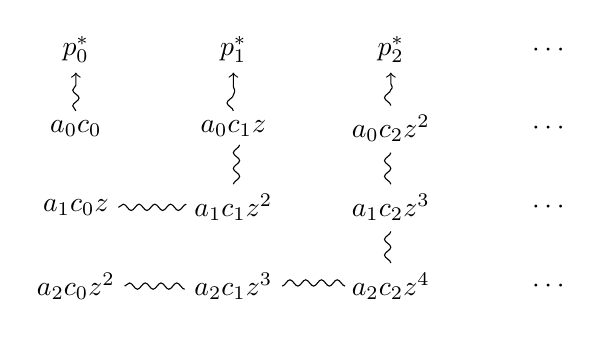
\begin{tikzpicture}
\pgfmathsetmacro{\Lx}{2}
\pgfmathsetmacro{\Ly}{1}
%
\draw(0,3*\Ly)node[](Aa){$p^*_0$}++(\Lx,0)node[](Ab){$p^*_1$}++(\Lx,0)node[](Ac){$p^*_2$}++(\Lx,0)node[](Ad){$\cdots$};
\draw(0,2*\Ly)node[](Ba){$a_0c_0$}++(\Lx,0)node[](Bb){$a_0c_1z$}++(\Lx,0)node[](Bc){$a_0c_2z^2$}++(\Lx,0)node[](Bd){$\cdots$};
\draw(0,\Ly)node[](Ca){$a_1c_0z$}++(\Lx,0)node[](Cb){$a_1c_1z^2$}++(\Lx,0)node[](Cc){$a_1c_2z^3$}++(\Lx,0)node[](Cd){$\cdots$};
\draw(0,0)node[](Da){$a_2c_0z^2$}++(\Lx,0)node[](Db){$a_2c_1z^3$}++(\Lx,0)node[](Dc){$a_2c_2z^4$}++(\Lx,0)node[](Dd){$\cdots$};
%
\draw[->,decorate,decoration={snake,amplitude=0.4mm,segment length=2mm,post length=1mm}](Ba)--(Aa);
\draw[->,decorate,decoration={snake,amplitude=0.4mm,segment length=2mm,post length=1mm}](Ca)--(Cb)--(Bb)--(Ab);
\draw[->,decorate,decoration={snake,amplitude=0.4mm,segment length=2mm,post length=1mm}](Da)--(Db)--(Dc)--(Cc)--(Bc)--(Ac);
\end{tikzpicture}
\caption{ثبوت مسئلہ \حوالہ{مسئلہ_ٹیلر_طاقتی_تسلسل_کا_کوشی_حاصل_ضرب}}
\label{شکل_مسئلہ_ٹیلر_طاقتی_تسلسل_کا_کوشی_حاصل_ضرب}
\end{figure}
\انتہا{ثبوت}
%=========================

\ابتدا{مثال}\quad \موٹا{کوشی حاصل ضرب}\\
ہندسی تسلسل \عددی{1+z+z^2+\cdots} کا \عددی{\abs{z}<1} کی صورت میں مجموعہ \عددی{\tfrac{1}{1-z}} ہے (حصہ \حوالہ{حصہ_ترتیب_تسلسل_آزمائش})۔مسئلہ \حوالہ{مسئلہ_ٹیلر_طاقتی_تسلسل_کا_کوشی_حاصل_ضرب} سے درج ذیل حاصل ہو گا۔
\begin{align*}
\big(\frac{1}{1-z}\big)^2&=\sum\limits_{k=0}^{\infty} z^k\sum\limits_{m=0}^{\infty} z^m=(1+z+z^2+\cdots)(1+z+z^2+\cdots)\\
&=1+2z+3z^2+\cdots=\sum\limits_{n=0}^{\infty}(n+1)z^n\quad \quad (\abs{z}<1)
\end{align*}
\انتہا{مثال}
%====================

\حصہء{سوالات}
%=====================
\ابتدا{سوال}\quad
اگر ترتیب \عددی{\abs{\tfrac{c_{n+1}}{c_n}}}، جہاں \عددی{n=1,2,\cdots} ہے، مرتکز ہو اور اس کا حد \عددی{L} ہو تب دکھائیں کہ طاقتی تسلسل (مساوات \حوالہ{مساوات_ٹیلر_طاقتی_تسلسل_الف}) کی ارتکاز کے دائرے کا رداس، \عددی{L>0} کی صورت میں \عددی{R=\tfrac{1}{L}}  ہو گا جبکہ \عددی{L=0} کی صورت میں \عددی{R=\infty} ہو گا۔
\انتہا{سوال}
%================
\ابتدا{سوال}\quad
اگر مساوات \حوالہ{مساوات_ٹیلر_طاقتی_تسلسل_ب} میں دی گئی تسلسل کی ارتکاز کا رداس (جو متناہی تصور  کیا گیا ہو)\عددی{R}  ہے، تب دکھائیں کہ \عددی{\sum c_mz^{2m}} کی ارتکاز کا رداس \عددی{\sqrt{R}} ہو گا۔
\انتہا{سوال}
%====================
سوال \حوالہ{سوال_ٹیلر_ارتکاز_کا_رداس_الف} تا سوال \حوالہ{سوال_ٹیلر_ارتکاز_کا_رداس_ب} میں ارتکاز کا رداس تلاش کریں۔

%======================
\ابتدا{سوال}\شناخت{سوال_ٹیلر_ارتکاز_کا_رداس_الف}\quad
$\sum\limits_{n=0}^{\infty} (z-i2)^n$\\
جواب:\quad
$1$
\انتہا{سوال}
%=============================
\ابتدا{سوال}\quad
$\sum\limits_{n=0}^{\infty} \tfrac{(z-2)^n}{2^n}$
\انتہا{سوال}
%=============================
\ابتدا{سوال}\quad
$\sum\limits_{n=0}^{\infty} n(\tfrac{z}{3})^n$\\
جواب:\quad
$3$
\انتہا{سوال}
%=============================
\ابتدا{سوال}\quad
$\sum\limits_{n=0}^{\infty} \tfrac{(2z)^n}{n!}$
\انتہا{سوال}
%=============================
\ابتدا{سوال}\quad
$\sum\limits_{n=0}^{\infty} \tfrac{z^{2n}}{n!}$\\
جواب:\quad
$\infty$
\انتہا{سوال}
%=============================
\ابتدا{سوال}\quad
$\sum\limits_{n=1}^{\infty} \tfrac{z^n}{n}$
\انتہا{سوال}
%=============================
\ابتدا{سوال}\quad
$\sum\limits_{n=0}^{\infty} \tfrac{(-1)^n}{n!}z^n$\\
جواب:\quad
$\infty$
\انتہا{سوال}
%=============================
\ابتدا{سوال}\quad
$\sum\limits_{n=0}^{\infty} \tfrac{n^2}{2^n}z^n$
\انتہا{سوال}
%=============================
\ابتدا{سوال}\quad
$\sum\limits_{n=0}^{\infty} \tfrac{(2n)!}{(n!)^2}z^n$\\
جواب:\quad
$\tfrac{1}{4}$
\انتہا{سوال}
%=============================
\ابتدا{سوال}\quad
$\sum\limits_{n=0}^{\infty} \tfrac{z^n}{n^n}$
\انتہا{سوال}
%=============================
\ابتدا{سوال}\quad
$\sum\limits_{n=0}^{\infty} \tfrac{(-1)^n}{(2n)!}z^{2n}$\\
جواب:\quad
$\infty$
\انتہا{سوال}
%=============================
\ابتدا{سوال}\quad
$\sum\limits_{n=1}^{\infty} \tfrac{z^n}{n^2}$
\انتہا{سوال}
%=============================
\ابتدا{سوال}\quad
$\sum\limits_{n=0}^{\infty} 6^n(z-i)^n$\\
جواب:\quad
$\tfrac{1}{6}$
\انتہا{سوال}
%=============================
\ابتدا{سوال}\quad
$\sum\limits_{n=0}^{\infty} (n!)^2 z^n$
\انتہا{سوال}
%=============================
\ابتدا{سوال}\quad
$\sum\limits_{n=0}^{\infty} 3^{2n}z^n$\\
جواب:\quad
$\tfrac{1}{9}$
\انتہا{سوال}
%=============================
\ابتدا{سوال}\شناخت{سوال_ٹیلر_ارتکاز_کا_رداس_ب}\quad
$\sum\limits_{n=0}^{\infty} \tfrac{\pi^n}{2^n}z^n$
\انتہا{سوال}
%=============================
\ابتدا{سوال}\quad
اگر \عددی{\sum c_nz^n} تمام متناہی \عددی{z} کے لئے مرتکز ہو تب دکھائیں کہ \عددی{n\to\infty} کے لئے 
$\,\sqrt[\leftroot{-2}n]{\abs{c_n}}\to 0\,$
ہو گا۔کوئی مثال پیش کریں۔
\انتہا{سوال}
%=====================
\ابتدا{سوال}\quad
ارتکاز کے دائرے پر تسلسل مرتکز یا منفرج ہو سکتا ہے۔ہندسی تسلسل کے لئے اس حقیقت کو دکھائیں۔
\انتہا{سوال}
%======================

\حصہ{طاقتی تسلسل کی روپ میں تفاعل}
اس حصے میں ہم دکھائیں گے کہ طاقتی تسلسل تحلیلی تفاعل کو ظاہر کرتی ہیں (مسئلہ \حوالہ{مسئلہ_ٹیلر_تحلیلی_تفاعل_تفرق})۔اس کا الٹ یعنی ہر تحلیلی تفاعل کو طاقتی تسلسل (جس کو ٹیلر تسلسل کہتے ہیں) سے ظاہر کیا جا سکتا ہے کو اگلے حصے میں ثابت کیا جائے گا۔ان دو وجوہات کی بنا طاقتی تسلسل مخلوط تجزیہ میں اہم کردار ادا کرتے ہیں۔

فرض کریں کہ 
$\,\sum_{n=0}^{\infty}c_nz^n\,$
اختیاری طاقتی تسلسل ہے جس کی ارتکاز کا رداس \عددی{R} غیر صفر ہے۔تب اس تسلسل کا مجموعہ \عددی{z} کا تفاعل ہو گا مثلاً \عددی{f(z)} جس کو ہم
\begin{align}\label{مساوات_ٹیلر_طاقتی_تسلسل_اور_تحلیلی_تفاعل_الف}
f(z)=\sum\limits_{n=0}^{\infty} c_nz^n =c_0+c_1z+c_2z^2+\cdots\quad\quad (\abs{z}<R)
\end{align}
لکھتے ہیں اور ہم کہتے ہیں کہ \عددی{f(z)} کو طاقتی تسلسل ظاہر کرتی ہے۔مثال کے طور پر اکائی دائرہ \عددی{\abs{z}=1} کے اندر  ہندسی تسلسل  تفاعل \عددی{f(z)=\tfrac{1}{1-z}} کو ظاہر کرتی ہے (مسئلہ \حوالہ{مسئلہ_ترتیب_ہندسی_تسلسل})۔

%======================
\ابتدا{مسئلہ}\شناخت{مسئلہ_ٹیلر_استمرار}\quad \موٹا{استمرار}\\
\عددی{R>0} کی صورت میں \عددی{z=0} پر  مساوات \حوالہ{مساوات_ٹیلر_طاقتی_تسلسل_اور_تحلیلی_تفاعل_الف} میں تفاعل \عددی{f(z)}  استمراری ہے۔
\انتہا{مسئلہ}
%=======================
\ابتدا{ثبوت}\quad
ہم درج ذیل دکھانا چاہتے ہیں۔
\begin{align}\label{مساوات_ٹیلر_طاقتی_تسلسل_اور_تحلیلی_تفاعل_ب}
\lim_{z\to 0} f(z)=f(0)=c_0
\end{align}
ہم اختیاری مثبت عدد \عددی{r<R} منتخب کرتے ہیں۔چونکہ مساوات \حوالہ{مساوات_ٹیلر_طاقتی_تسلسل_اور_تحلیلی_تفاعل_الف} میں دیا گیا تسلسل  قرص \عددی{\abs{z}<R} میں حتمی مرتکز ہے لہٰذا درج ذیل تسلسل مرتکز ہو گا۔
\begin{align*}
\sum\limits_{n=1}^{\infty}\abs{c_n}r^{n-1}=\frac{1}{r}\sum\limits_{n=1}^{\infty} \abs{c_n}r^n\quad \quad (0<r<R)
\end{align*}
فرض کریں کہ اس تسلسل کا مجموعہ \عددی{K} ہے۔تب ہمیں درج ذیل ملتا ہے۔
\begin{align*}
\abs{f(z)-c_0}=\abs{z\sum\limits_{n=1}^{\infty} c_n z^{n-1}}\le \abs{z}\sum\limits_{n=1}^{\infty}\abs{c_n}\abs{z}^{n-1}\le \abs{z}K\quad \quad (0<\abs{z}\le r)
\end{align*}
اب دیے گئے  \عددی{\epsilon>0} کے لئے، ان تمام \عددی{z} پر جو \عددی{\abs{z}<\sigma} کو مطمئن کرتے ہوں جہاں \عددی{\sigma} ایسا حقیقی مثبت عدد ہے جو \عددی{r} اور \عددی{\tfrac{\epsilon}{K}} دونوں سے چھوٹا ہو،  \عددی{\abs{f(z)-c_0}<\epsilon} ہو گا۔یوں حد کی تعریف کی رو سے مساوات \حوالہ{مساوات_ٹیلر_طاقتی_تسلسل_اور_تحلیلی_تفاعل_ب} مطمئن ہو گا لہٰذا مسئلے کا ثبوت مکمل ہوتا ہے۔ 
\انتہا{ثبوت}
%========================

ہم اب \اصطلاح{یکتائی}\فرہنگ{یکتائی}\فرہنگ{uniqueness} پر غور کرتے ہیں۔ہم دکھائیں گے کہ ایک ہی تفاعل \عددی{f(z)} کو ایک ہی مرکز والے دو مختلف طاقتی تسلسل سے ظاہر کرنا ممکن نہیں ہو گا۔اگر \عددی{f(z)} کو مرکز \عددی{a} کی طاقتی تسلسل سے ظاہر کیا جائے تب ایسا تسلسل یکتا ہو گا۔اس اہم حقیقت کی حقیقی اور مخلوط تجزیہ میں عموماً ضرورت پیش آتی ہے۔ہم اس کو درج ذیل مسئلہ میں پیش کرتے ہیں (جہاں عمومیت کھوئے بغیر \عددی{a=0} تصور کیا گیا ہے)۔ 

%====================
\ابتدا{مسئلہ}\شناخت{مسئلہ_ٹیلر_مماثلت}\quad \موٹا{طاقتی تسلسل کا مسئلہ مماثلت}\\
فرض کریں کہ مثبت \عددی{R} کے لئے تسلسل
\begin{align*}
\sum\limits_{n=0}^{\infty} a_n z^n \quad \text{اور}\quad \sum\limits_{n=0}^{\infty} b_n z^n
\end{align*}
\عددی{\abs{z}<R} پر مرتکز ہیں اور ان تمام \عددی{z} پر ان کا مجموعہ ایک جیسا ہے۔تب دونوں تسلسل مماثل ہوں گے یعنی تمام \عددی{n} کے لئے درج ذیل ہو گا۔
\begin{align}
a_n=b_n\quad \quad \quad n=0,1,\cdots
\end{align}
\انتہا{مسئلہ}
%========================
\ابتدا{ثبوت}\quad
ہم الکراجی ماخوذ\فرہنگ{الکراجی!ماخوذ} کی مدد سے آگے بڑھتے ہیں۔ہم درج ذیل فرض کرتے ہیں۔
\begin{align}\label{مساوات_ٹیلر_مسئلہ_مماثلت_الف}
a_0+a_1z+a_2z^2+\cdots=b_0+b_1z+b_2z^2+\cdots\quad \quad (\abs{z}<R)
\end{align}
\عددی{z} کو صفر تک پہنچانے سے مسئلہ \حوالہ{مسئلہ_ٹیلر_استمرار} کے تحت \عددی{a_0=b_0} ہو گا۔ہم فرض کرتے ہیں کہ \عددی{n=0,1,\cdots,m} کے لئے \عددی{a_n=b_n} ہیں۔تب مساوات \حوالہ{مساوات_ٹیلر_مسئلہ_مماثلت_الف} میں دونوں ہاتھ ابتدائی \عددی{m+1} اجزاء حذف کرنے کے بعد \عددی{z^{m+1}\,\,(\ne 0)} سے تقسیم کرتے ہوئے
\begin{align*}
a_{m+1}+a_{m+2}z+a_{m+3}z^2+\cdots=b_{m+1}+b_{m+2}z+b_{m+3}z^2+\cdots
\end{align*}
ملتا ہے۔ مسئلہ \حوالہ{مسئلہ_ٹیلر_استمرار} کے تحت دونوں میں سے ہر ایک تسلسل \عددی{z=0} پر استمراری تفاعل کو ظاہر کرتی ہے۔یوں \عددی{a_{m+1}=b_{m+1}} ہو گا۔یوں ثبوت مکمل ہوتا ہے۔
\انتہا{ثبوت}
%======================

آئیں اب طاقتی تسلسل کی جزو در جزو تفرق اور تکمل لینے پر غور کرتے ہیں۔تسلسل \عددی{c_1+c_1z+c_2z^2+\cdots} کا تفرق لینے سے درج ذیل تسلسل حاصل ہوتی ہے۔
\begin{align}\label{مساوات_ٹیلر_تفرقی_تسلسل}
\sum\limits_{n=1}^{\infty} nc_nz^{n-1}=c_1+2c_2z+3c_3z^2+\cdots
\end{align}
اس کو طاقتی تسلسل کی \اصطلاح{تفرقی تسلسل}\فرہنگ{تفرقی!تسلسل}\فرہنگ{تسلسل!تفرقی}\حاشیہب{derived series}\فرہنگ{series!derived} کہتے ہیں۔

%=====================
\ابتدا{مسئلہ}\شناخت{مسئلہ_ٹیلر_اصل_اور_تفرق_ایک_رداس_ارتکاز}\quad \موٹا{جزو در جزو تفرق}\\
تفرقی تسلسل کی ارتکاز کا رداس اصل تسلسل کی ارتکاز کے رداس کے برابر ہو گا۔
\انتہا{مسئلہ}
%============================
\ابتدا{ثبوت}\quad
فرض کریں کہ \عددی{nc_n=c^*_n} ہے۔تب
$\,\sqrt[\leftroot{-2}n]{\abs{c^*_n}}=\sqrt[\leftroot{-2}n]n\sqrt[\leftroot{-2}n]{\abs{c_n}}\,$
ہو گا۔چونکہ \عددی{n\to \infty} کرنے سے 
$\,\sqrt[\leftroot{-2}n]n\to 0\,$
ہو گا لہٰذا یا دونوں ترتیب 
$\,\sqrt[\leftroot{-2}n]{\abs{c^*_n}}\,$ 
اور
$\,\sqrt[\leftroot{-2}n]{\abs{c_n}}\,$ 
مرتکز ہوں گے اور ان کا ایک ہی حد ہو گا اور یا دونوں ترتیب منفرج ہوں گے۔اگر دونوں ترتیب منفرج ہوں ، تب دونوں یا غیر محدود ہوں گے یا دونوں محدود ہوں گے۔اگر دونوں محدود ہوں تب ان کے سب سے بڑے تحدیدی نقطے ایک جیسے ہوں گے۔ یوں اس سے اور مسئلہ \حوالہ{مسئلہ_ٹیلر_رداس_ارتکاز} سے موجودہ مسئلے کا فقرہ ثابت ہوتا ہے۔
\انتہا{ثبوت}
%======================
\ابتدا{مثال}\quad
طاقتی تسلسل
\begin{align*}
\sum\limits_{n=1}^{\infty} (n+1)z^n
\end{align*}
کی ارتکاز کا رداس \عددی{R=1} ہے۔ہندسی تسلسل کا تفرق لے کر مسئلہ \حوالہ{مسئلہ_ٹیلر_اصل_اور_تفرق_ایک_رداس_ارتکاز} کی اطلاق سے ایسا حاصل ہوتا ہے۔
\انتہا{مثال}
%======================
\ابتدا{مسئلہ}\شناخت{مسئلہ_ٹیلر_جزو_در_جزو_تکمل}\quad \موٹا{جزو در جزو تکمل}\\
تسلسل \عددی{c_0+c_1z+c_2z^2+\cdots} کا جزو در جزو تکمل لینے سے حاصل تسلسل
\begin{align*}
\sum\limits_{n=0}^{\infty} \frac{c_n}{n+1}z^{n+1}=c_0z+\frac{c_1}{2}z^2+\frac{c_2}{3}z^3+\cdots
\end{align*}
کی ارتکاز کا رداس اصل تسلسل کی ارتکاز کے رداس کے برابر ہو گا۔
\انتہا{مسئلہ}
%=====================
اس مسئلہ کا ثبوت مسئلہ \حوالہ{مسئلہ_ٹیلر_اصل_اور_تفرق_ایک_رداس_ارتکاز} کی ثبوت کی طرح ہے۔

طاقتی تسلسل تحلیلی تفاعل کو ظاہر کرتی ہیں اور تفرقی تسلسل (جو تسلسل کا جزو در جزو تفرق لے کر حاصل کیا جاتا ہے) ان تفاعل کی تفرق کو ظاہر کرتی ہیں۔

%=================
\ابتدا{مسئلہ}\شناخت{مسئلہ_ٹیلر_تحلیلی_تفاعل_تفرق}\quad \موٹا{تحلیلی تفاعل۔ ان کے تفرق}\\
غیر صفر رداس ارتکاز \عددی{R} والی طاقتی تسلسل دائرہ ارتکاز کے اندر ہر نقطہ پر تحلیلی تفاعل کو ظاہر کرتا ہے۔ان تفاعل کے بلند درجی تفرق حاصل کرنے کی خاطر اصل طاقتی تسلسل کے جزو در جزو تفرق لیے جاتے ہیں؛یوں حاصل تمام تسلسلوں کی ارتکاز کا رداس اصل تسلسل کی ارتکاز کے رداس جیسا ہو گا۔  
\انتہا{مسئلہ}
%========================
\ابتدا{ثبوت}\quad
ہم پہلے ثابت کرتے ہیں کہ کسی بھی عددی صحیح \عددی{n\ge 2} کے لئے
\begin{gather}
\begin{aligned}\label{مساوات_ٹیلر_تحلیلی_تفاعل_کے_تفرق_الف}
\text{(الف)}\quad &\frac{b^n-a^n}{b-a}-na^{n-1}=(b-a)A_n\\
\text{(ب)}\quad &A_n=b^{n-2}+2ab^{n-3}+3a^2b^{n-4}+\cdots+(n-1)a^{n-2}\quad \quad \text{\RL{ہو گا جہاں}}
\end{aligned}
\end{gather}

ہے۔ہم الکراجی ماخوذ کی مدد سے آگے بڑھتے ہیں۔سادہ حساب سے آپ دیکھ سکتے ہیں کہ \عددی{n=2} کے لئے مساوات \حوالہ{مساوات_ٹیلر_تحلیلی_تفاعل_کے_تفرق_الف} مطمئن ہوتی ہیں۔فرض کریں کہ \عددی{n=k} کے لئے مساوات \حوالہ{مساوات_ٹیلر_تحلیلی_تفاعل_کے_تفرق_الف} مطمئن ہوتی ہیں۔ہم دکھاتے ہیں کہ یہ \عددی{n=k+1} کے لئے بھی یہ مساوات مطمئن ہوں گی۔ ہم \عددی{n=k+1} کے لئے درج ذیل لکھتے ہیں۔
\begin{align*}
\frac{b^{k+1}-a^{k+1}}{b-a}=\frac{b^{k+1}-ba^k+ba^k-a^{k+1}}{b-a}=b\frac{b^k-a^k}{b-a}+a^k
\end{align*}
مساوات \حوالہ{مساوات_ٹیلر_تحلیلی_تفاعل_کے_تفرق_الف}-الف کے تحت دایاں ہاتھ درج ذیل کے برابر ہو گا
\begin{align*}
b[(b-a)A_k+ka^{k-1}]+a^k
\end{align*}
جس کو
\begin{align*}
(b-a)[bA_k+ka^{k-1}]+ka^k+a^k
\end{align*}
لکھا جا سکتا ہے۔\عددی{n=k} لیتے ہوئے  چکور قوسین میں بند حصے  کو مساوات \حوالہ{مساوات_ٹیلر_تحلیلی_تفاعل_کے_تفرق_الف}-ب سے 
\begin{align*}
b^{k-1}+2ab^{k-2}+\cdots+(k-1)b^{k-2}+ka^{k-1}=A_{k+1}
\end{align*}
لکھا جا سکتا ہے۔یوں ہمیں
\begin{align*}
\frac{b^{k+1}-a^{k+1}}{b-a}=(b-a)A_{k+1}+(k+1)a^k
\end{align*}
ملتا ہوتا ہے جو \عددی{n=k+1} لیتے ہوئے مساوات \حوالہ{مساوات_ٹیلر_تحلیلی_تفاعل_کے_تفرق_الف} ہے۔اس طرح کسی بھی \عددی{n\ge 2} کے لئے مساوات \حوالہ{مساوات_ٹیلر_تحلیلی_تفاعل_کے_تفرق_الف} ثابت ہوتا ہے۔

ہم اب مسئلہ \حوالہ{مسئلہ_ٹیلر_تحلیلی_تفاعل_تفرق} کے فقروں کو ثابت کرتے ہیں۔درج ذیل روپ پر غور کریں۔
\begin{align*}
f(z)=\sum\limits_{n=0}^{\infty} c_n z^n
\end{align*}
فرض کریں کہ اس کی  ارتکاز کا رداس \عددی{R} غیر صفر ہے۔ہم ثابت کرتے ہیں کہ کسی بھی مقررہ \عددی{z} جہاں \عددی{\abs{z}<R} ہے کے لئے \عددی{\Delta z\to 0} کرنے سے 
$\,\tfrac{f(z+\Delta z)-f(z)}{\Delta z}\,$
 کی قیمت تفرقی تسلسل مساوات \حوالہ{مساوات_ٹیلر_تفرقی_تسلسل} تک پہنچتی ہے جس کو ہم \عددی{f_1(z)} سے ظاہر کرتے ہیں۔جزو در جزو مجموعہ لے کر
\begin{align*}
\frac{f(z+\Delta z)-f(z)}{\Delta z}-f_1(z)=\sum\limits_{n=2}^{\infty} c_n\big[\frac{(z+\Delta z)^n-z^n}{\Delta z}-nz^{n-1}\big]
\end{align*}
لکھا جا سکتا ہے۔مساوات \حوالہ{مساوات_ٹیلر_تحلیلی_تفاعل_کے_تفرق_الف} میں \عددی{b=z+\Delta z}، \عددی{a=z} اور \عددی{b-a=\Delta z} لیتے ہوئے ہم دیکھتے ہیں کہ دائیں ہاتھ کا تسلسل
\begin{align*}
\Delta z\sum\limits_{n=2}^{\infty} c_n[(z+\Delta z)^{n-2}+2z(z+\Delta z)^{n-3}+\cdots+(n-1)z^{n-2}]
\end{align*} 
لکھا جا سکتا ہے اور \عددی{\abs{z}\le R_0} اور \عددی{\abs{z+\Delta z}\le R_0} جہاں \عددی{R_0<R} ہے کے لئے اس کی حتمی قیمت درج ذیل سے زیادہ نہیں ہو سکتی ہے
\begin{align}\label{مساوات_ٹیلر_دوسری_تفرقی_تسلسل}
\abs{\Delta z}\sum\limits_{n=2}^{\infty} \abs{c_n} n(n-1)R_0^{n-2}
\end{align}
جہاں عددی سر \عددی{1,2,\cdots,n-1} میں سب سے بڑا عددی سر \عددی{n-1} ہے اور  اجزاء کی تعداد \عددی{n} ہے۔ مساوات \حوالہ{مساوات_ٹیلر_دوسری_تفرقی_تسلسل} میں دیا گیا تسلسل   دوسری تفرقی تسلسل کے ساتھ \عددی{R_0} پر  قریبی تعلق رکھتا ہے۔بلکہ اس تفرقی مساوات کے عددی سر \عددی{c_n} ہیں (جبکہ مساوات \حوالہ{مساوات_ٹیلر_دوسری_تفرقی_تسلسل} کے تسلسل کے عددی سر \عددی{\abs{c_n}} ہیں) اور مسئلہ \حوالہ{مسئلہ_ٹیلر_اصل_اور_تفرق_ایک_رداس_ارتکاز} اور مسئلہ \حوالہ{مسئلہ_ٹیلر_طاقتی_تسلسل_کی_مرکوزیت} کے تحت  \عددی{R_0\,(<R)} پر حتمی مرتکز ہے۔ اس سے مراد مساوات \حوالہ{مساوات_ٹیلر_دوسری_تفرقی_تسلسل} کے تسلسل کی \عددی{R_0} پر مرکوزیت ہے؛ فرض کریں کہ اس کی قیمت \عددی{K(R_0)} ہے، تب ہمارا نتیجہ درج  ذیل لکھا جا سکتا ہے۔
\begin{align*}
\abs{\frac{f(z+\Delta z)-f(z)}{\Delta z}-f_1(z)}\le \abs{\Delta z} K(R_0)
\end{align*}
\عددی{\Delta \to 0} لیتے ہوئے اور جانتے ہوئے کہ \عددی{R_0\,(<R)} اختیاری ہے، ہم دیکھ سکتے ہیں کہ دائرہ ارتکاز کے اندر کسی بھی نقطہ پر \عددی{f(z)} تحلیلی ہو گا اور اس کے تفرق کو تفرقی تسلسل ظاہر کرے گا۔اس سے بلند درجی تفرق کا فقرہ الکراجی ماخوذ سے اخذ کیا جا سکتا ہے۔یوں  مسئلہ \حوالہ{مسئلہ_ٹیلر_تحلیلی_تفاعل_تفرق} کا ثبوت مکمل ہوتا ہے۔
\انتہا{ثبوت}
%=====================

مسئلہ \حوالہ{مسئلہ_ٹیلر_تحلیلی_تفاعل_تفرق}  سے ہم دیکھتے ہیں کہ \عددی{f(z)} (مساوات \حوالہ{مساوات_ٹیلر_طاقتی_تسلسل_اور_تحلیلی_تفاعل_الف}) کا \عددی{m} واں تفرق \عددی{f^{(m)}(z)} درج ذیل ہو گا۔
\begin{align}
f^{(m)}(z)=\sum\limits_{n=m}^{\infty} n(n-1)\cdots(n-m+1)c_nz^{n-m}\quad (\abs{z}<R)
\end{align}
اگلے حصے میں ہم دیکھیں گے کہ ہر تحلیلی تفاعل کو طاقتی تسلسل ظاہر کر سکتا ہے۔

%=====================
\حصہء{سوالات}
%===================
\ابتدا{سوال}\quad
اگر مساوات \حوالہ{مساوات_ٹیلر_طاقتی_تسلسل_اور_تحلیلی_تفاعل_الف} میں دیا گیا تسلسل جفت ہو تب ثابت کریں کہ طاق \عددی{n} کے \عددی{c_n}  صفر ہوں گے۔ (مسئلہ \حوالہ{مسئلہ_ٹیلر_مماثلت} استعمال کریں۔)
\انتہا{سوال}
%====================
\ابتدا{سوال}\quad
اگر مساوات \حوالہ{مساوات_ٹیلر_طاقتی_تسلسل_اور_تحلیلی_تفاعل_الف} میں دیا گیا تسلسل طاق ہو تب ثابت کریں کہ جفت \عددی{n} کے \عددی{c_n}  صفر ہوں گے۔ مثال پیش کریں۔
\انتہا{سوال}
%===================
\ابتدا{سوال}\quad
مسئلہ \حوالہ{مسئلہ_ٹیلر_مماثلت} کا اطلاق 
$\,(1+z)^p(1+z)^q=(1+z)^{p+q}\,$
پر کرتے ہوئے درج ذیل حاصل کریں جہاں \عددی{p} اور \عددی{q} مثبت عدد صحیح ہیں۔
\begin{align*}
\sum\limits_{n=0}^{\infty}
\begin{pmatrix}
p\\
n
\end{pmatrix}
\begin{pmatrix}
q\\
r-n
\end{pmatrix}=
\begin{pmatrix}
p+q\\
r
\end{pmatrix}
\end{align*}
\انتہا{سوال}
%======================
\ابتدا{سوال}\quad 
ہندسی تسلسل کے لئے مسئلہ \حوالہ{مسئلہ_ٹیلر_اصل_اور_تفرق_ایک_رداس_ارتکاز} اور مسئلہ \حوالہ{مسئلہ_ٹیلر_جزو_در_جزو_تکمل} کی تصدیق کریں۔
\انتہا{سوال}
%==========================
ہندسی تسلسل پر مسئلہ \حوالہ{مسئلہ_ٹیلر_اصل_اور_تفرق_ایک_رداس_ارتکاز} اور مسئلہ \حوالہ{مسئلہ_ٹیلر_جزو_در_جزو_تکمل} کے اطلاق سے سوال \حوالہ{سوال_ٹیلر_رداس_ارتکاز_الف} تا سوال \حوالہ{سوال_ٹیلر_رداس_ارتکاز_ب} میں دیے تسلسل کی ارتکاز کا رداس تلاش کریں۔ 

%====================
\ابتدا{سوال}\شناخت{سوال_ٹیلر_رداس_ارتکاز_الف}\quad
$\sum\limits_{n=1}^{\infty}\tfrac{n}{5^n}(z-i)^n$\\
جواب:\quad
$5$

\انتہا{سوال}
%====================
\ابتدا{سوال}\quad
$\sum\limits_{n=1}^{\infty} \tfrac{(z+2)^n}{n}$
\انتہا{سوال}
%====================
\ابتدا{سوال}\quad
$\sum\limits_{n=1}^{\infty} \tfrac{4^n}{n}(z+i2)^n$\\
جواب:\quad
$\tfrac{1}{4}$
\انتہا{سوال}
%====================
\ابتدا{سوال}\quad
\begin{align*}
\sum\limits_{n=k}^{\infty}
\begin{pmatrix}
n\\
k
\end{pmatrix}
\big(\frac{z}{2}\big)^n
\end{align*}
\انتہا{سوال}
%====================
\ابتدا{سوال}\quad
\begin{align*}
\sum\limits_{n=0}^{\infty}
\left[\begin{pmatrix} n+k\\n  \end{pmatrix}\right]^{-1} z^{n+k}
\end{align*}
جواب:\quad 
$1$
\انتہا{سوال}
%====================
\ابتدا{سوال}\شناخت{سوال_ٹیلر_رداس_ارتکاز_ب}\quad
\begin{align*}
\sum\limits_{n=0}^{\infty}
\left[\begin{pmatrix} n+k\\n  \end{pmatrix}\right]^{-1} \big(\frac{z}{3}\big)^n
\end{align*}
\انتہا{سوال}
%====================

\حصہ{ٹیلر تسلسل}\شناخت{حصہ_ٹیلر_تسلسل}
حقیقی علم الاحصاء میں ٹیلر تسلسل انتہائی طاقتور ثابت ہوتا ہے۔ہم اب دیکھیں گے کہ مخلوط تجزیہ میں اس کی عمومی صورت پائی جاتی ہے جو اس سے بھی زیادہ اہم ہے۔

آئیں نقطہ \عددی{z=a} کی پڑوس میں تحلیلی تفاعل \عددی{f(z)} پر غور کرتے ہیں۔فرض کریں کہ اس پڑوس میں دائرہ \عددی{C} پایا جاتا ہے جس کا مرکز \عددی{a} ہے۔ہم \عددی{z_0} اور \عددی{z} کی جگہ بالترتیب \عددی{z} اور \عددی{z^*} لکھتے ہوئے  کوشی کا کلیہ تکمل (مساوات \حوالہ{مساوات_مخلوط_تکمل_کوشی_کلیہ_تکمل_الف}) استعمال کرتے ہیں
\begin{align}\label{مساوات_ٹیلر_کوشی_کلیہ_تکمل_ٹیلر_الف}
f(z)=\frac{1}{i2\pi}\int\limits_C\frac{f(z^*)}{z^*-z}\dif z^*
\end{align}
جہاں \عددی{C} کے اندر \عددی{z} اختیاری مقررہ نقطہ ہے اور \عددی{z^*} مخلوط تکمل کا متغیرہ ہے (شکل \حوالہ{شکل_مساوات_ٹیلر_کوشی_کلیہ_تکمل_ٹیلر_الف})۔ہم اب مساوات \حوالہ{مساوات_ٹیلر_کوشی_کلیہ_تکمل_ٹیلر_الف} میں \عددی{\tfrac{1}{z^*-z}} کی طاقتی تسلسل \عددی{z-a} کی صورت میں حاصل کرتے ہیں۔ہم پہلے درج ذیل لکھتے ہیں۔
\begin{align}\label{مساوات_ٹیلر_کوشی_کلیہ_تکمل_ٹیلر_ب}
\frac{1}{z^*-z}=\frac{1}{z^*-a-(z-a)}=\frac{1}{(z^*-a)\big(1-\frac{z-a}{z^*-a}\big)}
\end{align}
چونکہ \عددی{z^*} دائرہ \عددی{C} پر پایا جاتا ہے جبکہ \عددی{z} دائرے کے اندر پایا جاتا ہے لہٰذا
\begin{align}\label{مساوات_ٹیلر_کوشی_کلیہ_تکمل_ٹیلر_پ}
\abs{\frac{z-a}{z^*-a}}<1
\end{align}
ہو گا۔
\begin{figure}
\centering
\begin{tikzpicture}
\draw(0,0)--++(2.5,0)node[right]{$x$};
\draw(0,0)node[ocirc]{}--++(0,2)node[left]{$y$};
\draw(1.25,1)node[ocirc]{}node[below]{$a$} circle (0.75);
\draw(1.25,1)++(30:0.75)node[ocirc,fill]{}node[right]{$z^*$};
\draw(1.25,1)++(130:0.5)node[ocirc]{}node[right]{$z$};
\draw(1.25,1)++(-20:0.75)node[right]{$C$};
\end{tikzpicture}
\caption{شکل برائے مساوات \حوالہ{مساوات_ٹیلر_کوشی_کلیہ_تکمل_ٹیلر_الف}}
\label{شکل_مساوات_ٹیلر_کوشی_کلیہ_تکمل_ٹیلر_الف}
\end{figure}

ہندسی تسلسل سے
\begin{align*}
1+q+q^2+\cdots+q^n=\frac{1-q^{n+1}}{1-q}\quad \quad \quad (q\ne 1)
\end{align*}
لکھتے ہوئے 
\begin{align*}
\frac{1}{1-q}=1+q+\cdots+q^n+\frac{q^{n+1}}{1-q}
\end{align*}
حاصل ہوتا ہے جس میں \عددی{q=\tfrac{z-a}{z^*-a}} پر کرنے سے
\begin{align*}
\frac{1}{1-\frac{z-a}{z^*-a}}=1+\frac{z-a}{z^*-a}+\big(\frac{z-a}{z^*-a}\big)^2+\cdots+\big(\frac{z-a}{z^*-a}\big)^n+\frac{\big(\frac{z-a}{z^*-a}\big)^{n+1}}{\frac{z-a}{z^*-a}}
\end{align*}
ملتا ہے۔ہم اس کو مساوات \حوالہ{مساوات_ٹیلر_کوشی_کلیہ_تکمل_ٹیلر_ب} میں پر کرنے کے بعد مساوات \حوالہ{مساوات_ٹیلر_کوشی_کلیہ_تکمل_ٹیلر_ب} کو مساوات \حوالہ{مساوات_ٹیلر_کوشی_کلیہ_تکمل_ٹیلر_الف} میں پر کرتے ہیں۔ چونکہ \عددی{z} اور \عددی{a} مستقل ہیں لہٰذا ہم \عددی{z-a} کی طاقتوں کو تکمل کی علامت سے باہر نکال سکتے ہیں۔یوں مساوات \حوالہ{مساوات_ٹیلر_کوشی_کلیہ_تکمل_ٹیلر_الف} درج ذیل صورت اختیار کرتی ہے
\begin{multline}\label{مساوات_ٹیلر_کوشی_کلیہ_تکمل_ٹیلر_ت}
f(z)=\frac{1}{i2\pi}\int\limits_C \frac{f(z^*)}{z^*-a}\dif z^*+\frac{z-a}{i2\pi}\int\limits_C \frac{f(z^*)}{(z^*-a)^2}\dif z^*+\cdots\\
+\frac{(z-a)^n}{i2\pi}\int\limits_C \frac{f(z^*)}{(z^*-a)^{n+1}}\dif z^*+R_n(z)
\end{multline}
جہاں آخری جزو درج ذیل کلیہ دیتی ہے۔
\begin{align}\label{مساوات_ٹیلر_کوشی_کلیہ_تکمل_ٹیلر_ٹ}
R_n(z)=\frac{(z-a)^{n+1}}{i2\pi}\int\limits_C \frac{f(z^*)}{(z^*-a)^{n+1}(z^*-z)}\dif z^*
\end{align}
مساوات \حوالہ{مساوات_مخلوط_تکمل_تحلیلی_تفاعل_کے_تفرق} استعمال کرتے ہوئے ہم مساوات \حوالہ{مساوات_ٹیلر_کوشی_کلیہ_تکمل_ٹیلر_ت} کو
\begin{align}\label{مساوات_ٹیلر_کوشی_کلیہ_تکمل_ٹیلر_ث}
f(z)=f(a)+\frac{z-a}{1!}f'(a)+\frac{(z-a)^2}{2!}f''(a)+\cdots+\frac{(z-a)^n}{n!}f^{(n)}(a)+R_n(z)
\end{align}
لکھ سکتے ہیں جو \اصطلاح{کلیہ ٹیلر}\فرہنگ{ٹیلر!کلیہ}\حاشیہب{Taylor's formula}\فرہنگ{Taylor!formula} کہلاتا\حاشیہد{انگلستانی ریاضی دان بروک ٹیلر [1685-1731]} ہے جبکہ \عددی{R_n(z)} کو \ترچھا{باقی}\فرہنگ{باقی} کہتے ہیں۔چونکہ تحلیلی تفاعل \عددی{f(z)} کا ہر درجے کا تفرق پایا جاتا ہے لہٰذا ہم مساوات \حوالہ{مساوات_ٹیلر_کوشی_کلیہ_تکمل_ٹیلر_ث} میں \عددی{n} جتنا چاہیں بڑا لے سکتے ہیں۔مساوات \حوالہ{مساوات_ٹیلر_کوشی_کلیہ_تکمل_ٹیلر_ث} میں \عددی{n\to \infty} کرنے سے 
\begin{align}\label{مساوات_ٹیلر_کوشی_کلیہ_تکمل_ٹیلر_ج}
f(z)=\sum\limits_{m=0}^{\infty} \frac{f^{(m)}(a)}{m!}(z-a)^m
\end{align}
حاصل ہوتا ہے۔مساوات \حوالہ{مساوات_ٹیلر_کوشی_کلیہ_تکمل_ٹیلر_ج} کو \عددی{f(z)} کا \اصطلاح{ٹیلر تسلسل}\فرہنگ{ٹیلر!تسلسل}\فرہنگ{تسلسل!ٹیلر}\حاشیہب{Taylor series}\فرہنگ{Taylor!series} کہتے ہیں جس کا \ترچھا{مرکز} \عددی{a} ہے۔اس کی وہ مخصوص صورت جس میں \عددی{a=0} ہو \عددی{f(z)} کا  \اصطلاح{مکلارن تسلسل}\فرہنگ{مکلارن!تسلسل}\فرہنگ{تسلسل!مکلارن}\حاشیہب{Maclaurin series}\فرہنگ{Maclaurin!series} کہلاتا\حاشیہد{اسکاچی ریاضی دان کولن مکلارن [1698-1746]} ہے۔ 

ظاہر ہے کہ مساوات \حوالہ{مساوات_ٹیلر_کوشی_کلیہ_تکمل_ٹیلر_ج} میں دیا گیا تسلسل اس صورت مرتکز ہو گا اور \عددی{f(z)} کو ظاہر کرے گا جب درج ذیل ہو۔
\begin{align}\label{مساوات_ٹیلر_کوشی_کلیہ_تکمل_ٹیلر_چ}
\lim_{n\to\infty} R_n(z)=0
\end{align}
مساوات \حوالہ{مساوات_ٹیلر_کوشی_کلیہ_تکمل_ٹیلر_چ} کو ثابت کرنے کی خاطر ہم مساوات \حوالہ{مساوات_ٹیلر_کوشی_کلیہ_تکمل_ٹیلر_ٹ} پر غور کرتے ہیں۔چونکہ \عددی{z^*} دائرہ \عددی{C} پر ہے جبکہ \عددی{z} اس دائرے کے اندر ہے لہٰذا \عددی{\abs{z^*-z}>0} ہو گا۔چونکہ \عددی{f(z)} دائرہ \عددی{C} پر اور اس دائرے کے اندر تحلیلی ہے لہٰذا 
$\,\tfrac{f(z^*)}{z^*-z}\,$
کی حتمی قیمت محدود ہو گی، مثلاً \عددی{C} پر تمام \عددی{z^*} کے لئے درج ذیل ہو گا۔ 
\begin{align*}
\abs{\frac{f(z^*)}{z^*-z}}<\tilde{M}
\end{align*}
فرض کریں کہ \عددی{C} کا رداس \عددی{r} ہے۔ تب \عددی{C} پر تمام \عددی{z^*} کے لئے  \عددی{\abs{z^*-a}=r} ہو گا جبکہ \عددی{C} کی لمبائی \عددی{2\pi r} ہو گی۔یوں مساوات \حوالہ{مساوات_ٹیلر_کوشی_کلیہ_تکمل_ٹیلر_ٹ} پر مساوات \حوالہ{مساوات_مخلوط_تکمل_حتمی_قیمت_تخمینہ} کا اطلاق کرتے ہوئے 
\begin{align*}
\abs{R_n}&=\frac{\abs{z-a}^{n+1}}{2\pi}\abs{\int\limits_C \frac{f(z^*)}{(z^*-a)^{n+1}(z^*-z)}\dif z^*}\\[0.5em]
&<\frac{\abs{z-a}^{n+1}}{2\pi} \tilde{M}\frac{1}{r^{n+1}}2\pi r=\tilde{M} r\abs{\frac{z-a}{r}}^{n+1}
\end{align*}
ملتا ہے۔اب \عددی{n} کی قیمت لامتناہی تک پہنچانے سے دایاں ہاتھ، مساوات \حوالہ{مساوات_ٹیلر_کوشی_کلیہ_تکمل_ٹیلر_پ} کے تحت، صفر تک پہنچے گا۔یوں  \عددی{C} کے اندر تمام \عددی{z} کے لئے مساوات \حوالہ{مساوات_ٹیلر_کوشی_کلیہ_تکمل_ٹیلر_چ} ثابت ہوتا ہے۔چونکہ مسئلہ \حوالہ{مسئلہ_ٹیلر_مماثلت} کے تحت \عددی{f(z)} کا مساوات \حوالہ{مساوات_ٹیلر_کوشی_کلیہ_تکمل_ٹیلر_ج} کی روپ میں اظہار یکتا ہے، یعنی مساوات \حوالہ{مساوات_ٹیلر_کوشی_کلیہ_تکمل_ٹیلر_ج} وہ واحد طاقتی تسلسل ہے جس کا مرکز \عددی{a} ہے اور جو \عددی{f(z)} کو ظاہر کرتا ہے لہٰذا ہم حاصل نتیجہ کو درج ذیل مسئلہ کو صورت میں بیان کر سکتے ہیں۔

%=======================
\ابتدا{مسئلہ}\شناخت{مسئلہ_ٹیلر_مسئلہ_ٹیلر}\quad \موٹا{مسئلہ ٹیلر}\\
فرض کریں کہ دائرہ کار \عددی{D} میں \عددی{f(z)} تحلیلی ہے اور \عددی{D} میں \عددی{z=a} کوئی نقطہ ہے۔تب ایسا واحد ایک طاقتی تسلسل موجود ہو گا جس کا مرکز \عددی{a} ہو اور جو \عددی{f(z)} کو ظاہر کرتا ہو؛ اس تسلسل کی روپ
\begin{align}\label{مساوات_ٹیلر_ٹیلر_تسلسل}
f(z)=\sum\limits_{n=0}^{\infty} b_n(z-a)^n
\end{align}
ہے جہاں
\begin{align*}
b_n=\frac{1}{n!}f^{(n)}(a)\quad \quad \quad n=0,1,\cdots
\end{align*}
ہے؛\عددی{D} میں اس بڑے سے بڑے کھلے قرص جس کا مرکز \عددی{a} ہو میں یہ تسلسل کارآمد ہو گا۔مساوات \حوالہ{مساوات_ٹیلر_ٹیلر_تسلسل} کے باقی \عددی{R_n(z)} کو  مساوات \حوالہ{مساوات_ٹیلر_کوشی_کلیہ_تکمل_ٹیلر_ٹ} ظاہر کرتی ہے۔ تسلسل کے عددی سر  عدم مساوات 
\begin{align}\label{مساوات_ٹیلر_ٹیلر_عددی_سر_عدم_مساوات}
\abs{b_n}\le \frac{M}{r^n}
\end{align}
کو مطمئن کرتے ہیں جہاں دائرہ \عددی{\abs{z-a}=r} پر \عددی{\abs{f(z)}} کی زیادہ سے زیادہ قیمت \عددی{M} ہے۔ 
\انتہا{مسئلہ}
%============================  

کوشی عدم مساوات \حوالہ{مساوات_مخلوط_تکمل_کوشی_عدم_مساوات} سے عدم مساوات \حوالہ{مساوات_ٹیلر_ٹیلر_عددی_سر_عدم_مساوات}  حاصل ہوتی ہے۔

عملاً مساوات \حوالہ{مساوات_ٹیلر_کوشی_کلیہ_تکمل_ٹیلر_چ} کہتی ہے کہ ان تمام \عددی{z} کے لئے جن پر مساوات \حوالہ{مساوات_ٹیلر_ٹیلر_تسلسل} منفرج ہو، مساوات \حوالہ{مساوات_ٹیلر_ٹیلر_تسلسل} کے \عددی{n} ویں جزوی مجموعہ کی قیمت \عددی{f(z)} کی قیمت کے اتنی قریب ہو گی جتنا درکار ہو، پس ہمیں \عددی{n} اتنا بڑا لینا ہو گا۔

ہم مسئلہ ٹیلر سے دیکھتے ہیں کہ مساوات \حوالہ{مساوات_ٹیلر_ٹیلر_تسلسل} کی ارتکاز کا رداس کم از کم \عددی{a} سے \عددی{D} کی سرحد تک کم سے کم فاصلہ جتنا ہو گا۔اگرچہ رداس  ارتکاز اس سے بڑا ہو سکتا ہے لیکن تب \عددی{D} کی ان تمام نقطوں پر جو ارتکاز کے دائرے کے اندر  پائے جاتے ہوں پر ضروری نہیں ہے کہ تسلسل \عددی{f(z)} کو ظاہر کرتا ہو۔ 

مخلوط تحلیلی تفاعل کی ایک انوکھی خاصیت یہ ہے کہ ان کی ہر درجے کے تفرق پائے جاتے ہیں اور اب ہم نے ان کی دوسری انوکھی خاصیت دریافت کی ہے کہ ان کو ہر صورت مساوات \حوالہ{مساوات_ٹیلر_ٹیلر_تسلسل} میں دی گئی طاقتی تسلسل کی روپ میں ظاہر کیا جا سکتا ہے۔حقیقی تفاعل کے لئے عموماً ایسا درست نہ ہو گا۔ایسے حقیقی تفاعل پائے جاتے ہیں جن کے ہر درجے کے تفرق پائے جاتے ہیں لیکن انہیں طاقتی تسلسل سے ظاہر کرنا ممکن نہیں ہے؛ مثلاً \عددی{f(x)=e^{-\tfrac{1}{x^2}}} جب \عددی{x\ne 0} ہو اور \عددی{f(z)=0} جب \عددی{x=0} ہو۔

ہماری موجودہ اور گزشتہ حصے کے  طاقتی تسلسل کے تبصروں کے مابین درج ذیل مسئلہ تعلق پیش کرتا ہے۔

%=================
\ابتدا{مسئلہ}\شناخت{مسئلہ_ٹیلر_یکتائی_ٹیلر_تسلسل}
غیر صفر ارتکاز کے رداس والا ہر وہ طاقتی تسلسل جو تفاعل کو ظاہر کرتا ہے، اس تفاعل کا ٹیلر تسلسل ہو گا۔ 
\انتہا{مسئلہ}
%========================
\ابتدا{ثبوت}\quad
فرض کریں کہ درج ذیل طاقتی تسلسل کا غیر صفر رداس ارتکاز \عددی{R} ہو۔
\begin{align*}
\sum\limits_{n=0}^{\infty}b_n(z-a)^n
\end{align*}
تب یہ قرص \عددی{\abs{z-a}<R} میں کسی تفاعل \عددی{f(z)} کو ظاہر کرے گا یعنی:
\begin{align*}
f(z)=b_0+b_1(z-a)+b_2(z-a)^2+\cdots
\end{align*}
مسئلہ \حوالہ{مسئلہ_ٹیلر_تحلیلی_تفاعل_تفرق} کے تحت
\begin{align*}
f'(z)=b_1+2b_2(z-a)+\cdots
\end{align*}
اور
\begin{align*}
f^{(n)}(z)=n!b_n+(n+1)n\cdots 3\cdot 2\cdot b_{n+1}(z-a)+\cdots
\end{align*}
ہو گا اور یہ تمام تسلسل قرص \عددی{\abs{z-a}<R} میں مرتکز ہوں گے اور تحلیلی تفاعل کو ظاہر کریں گے۔یوں یہ تفاعل \عددی{z=a} پر استمراری  ہوں گے۔یوں \عددی{z=a} لیتے ہوئے 
\begin{align*}
f(a)=b_0,\quad f'(a)=b_1,\quad \cdots,\quad f^{(n)}(a)=n!b_n,\cdots
\end{align*}
ملتے ہیں۔ چونکہ یہ کلیات مسئلہ ٹیلر  کے کلیات کے  عین مطابق ہیں لہٰذا ثبوت مکمل ہوتا ہے۔
\انتہا{ثبوت}
%=========================

وہ نقطہ جس پر تفاعل \عددی{f(z)} غیر تحلیلی صورت اختیار کرے \عددی{f(z)} کا \اصطلاح{نادر نقطہ}\فرہنگ{نادر نقطہ}\حاشیہب{singular point}\فرہنگ{singular point} کہلاتا ہے؛ ہم کہتے ہیں کہ اس نقطہ پر \عددی{f(z)} کی \اصطلاح{ندرت}\فرہنگ{ندرت}\حاشیہب{singularity}\فرہنگ{singularity} پائی جاتی ہے۔یہ کہنا زیادہ درست ہو گا کہ وہ نقطہ \عددی{z=z_0} جس پر \عددی{f(z)} قابل تفرق نہ ہو لیکن \عددی{z_0} کے ہر پڑوس میں \عددی{f(z)} قابل تفرق ہو تب \عددی{z_0} کو \عددی{f(z)} کا \ترچھا{نادر نقطہ} کہیں گے۔ 

اس تصور کے تحت دائرہ ارتکاز\حاشیہد{مساوات \حوالہ{مساوات_ٹیلر_ٹیلر_تسلسل} کا رداس ارتکاز عموماً \عددی{a} سے \عددی{f(z)} کے قریب ترین نادر نقطے تک فاصلے کے برابر ہو گا، لیکن  اس سے زیادہ بھی ہو سکتا ہے؛مثال کے طور پر \عددی{\Ln z} منفی حقیقی محور پر نادر ہے اور \عددی{a=-1+i} سے اس منفی محور تک فاصلہ \عددی{1} ہے لیکن \عددی{\Ln z} کا ٹیلر تسلسل جس کا مرکز \عددی{a=-1+i} ہو کی ارتکاز کا رداس \عددی{\sqrt{2}} ہے۔} پر \عددی{f(z)} (کی طاقتی تسلسل مساوات \حوالہ{مساوات_ٹیلر_ٹیلر_تسلسل}) کا کم از کم ایک نادر نقطہ پایا جائے گا۔ 

ٹیلر تسلسل کی عملی استعمال سے پہلے مختلف مرکزی نقطوں کے گرد تسلسل کی تصور  اور تحلیلی استمرار کی تصور  پر بھی بات کرتے ہیں۔فرض کریں غیر صفر رداس ارتکاز \عددی{R} کے تفاعل \عددی{f(z)} کا \عددی{z-a} طاقتوں کا طاقتی تسلسل  دیا گیا ہے جس کے مجموعہ کو ہم \عددی{f(z)} سے ظاہر کرتے ہیں یعنی؛
\begin{align}\label{مساوات_ٹیلر_دیا_گیا_الف}
f(z)=\sum\limits_{n=0}^{\infty} b_n(z-a)^n
\end{align}
مسئلہ \حوالہ{مسئلہ_ٹیلر_تحلیلی_تفاعل_تفرق} سے ہم جانتے ہیں کہ  قرص \عددی{\abs{z-a}<R} میں \عددی{f(z)} تحلیلی ہو گا۔مسئلہ \حوالہ{مسئلہ_ٹیلر_یکتائی_ٹیلر_تسلسل} کے تحت مساوات \حوالہ{مساوات_ٹیلر_دیا_گیا_الف} تفاعل \عددی{f(z)} کا ایسا ٹیلر تسلسل ہو گا جس کا مرکز \عددی{a} ہے۔ہم اس قرص میں کوئی نقطہ \عددی{b} منتخب کرتے ہوئے مسئلہ ٹیلر کی مدد سے  \عددی{f(z)} کے لئے 
\begin{align}\label{مساوات_ٹیلر_دیا_گیا_ب}
f(z)=\sum\limits_{n=0}^{\infty} b_n(z-b)^n
\end{align}
حاصل کرتے ہیں جس کے عددی سر  مساوات \حوالہ{مساوات_ٹیلر_دیا_گیا_الف} کے تفرق میں \عددی{z=b} پر کرنے سے حاصل ہوں گے:
\begin{align*}
b_n=\frac{1}{n!}f^{(n)}(b)=\sum\limits_{k=n}^{\infty} \begin{pmatrix} n\\k\end{pmatrix} a_k (b-a)^{k-n}
\end{align*}
یہ نئی تسلسل کم از کم قرص \عددی{\abs{z-b}<R-\abs{b}} میں کارآمد ہو گی (شکل \حوالہ{شکل_ٹیلر_مختلف_مرکز_تسلسل}-الف)۔البتہ کئی بار مساوات \حوالہ{مساوات_ٹیلر_دیا_گیا_ب} کی ارتکاز کا رداس \عددی{R-\abs{b}} سے بڑا ہو گا  (شکل \حوالہ{شکل_ٹیلر_مختلف_مرکز_تسلسل}-ب) لہٰذا  مساوات \حوالہ{مساوات_ٹیلر_دیا_گیا_ب} تفاعل \عددی{f(z)} کو  قرص \عددی{\abs{z-a}<R} کے باہر وسعت دے گی (شکل \حوالہ{شکل_ٹیلر_مختلف_مرکز_تسلسل}-ب میں سیاہ خطہ)۔کسی ارتکازی خطے میں ایک تحلیلی تفاعل کی دی گئی طاقتی تسلسل  کو اس خطے سے باہر وسعت دینے کو \اصطلاح{تحلیلی استمرار}\فرہنگ{تحلیلی!استمرار}\حاشیہب{analytic continuation}\فرہنگ{analytic!continuation} کہتے ہیں۔
\begin{figure}
\centering
\begin{subfigure}{0.5\textwidth}
\centering
\begin{tikzpicture}
\pgfmathsetmacro{\klen}{0.35}
\draw(0,0)node[ocirc]{}node[below]{$a$}circle (1);
\draw(0,0)++(30:1-\klen) node[ocirc]{}node[left]{$b$} circle (\klen);
\end{tikzpicture}
\caption*{(الف)}
\end{subfigure}%
\begin{subfigure}{0.5\textwidth}
\centering
\begin{tikzpicture}
\pgfmathsetmacro{\klen}{0.75}
\fill[gray!20!white](0,0)++(30:0.4) node[ocirc]{}node[right]{$b$} circle (\klen);
\fill[white](0,0)node[ocirc]{}node[shift={(-45:0.25)}]{$a$}circle (1);
\draw(0,0)node[ocirc]{}node[shift={(-45:0.25)}]{$a$}circle (1);
\draw(0,0)++(30:0.4) node[ocirc]{}node[right]{$b$} circle (\klen);
\end{tikzpicture}
\caption*{(ب)}
\end{subfigure}%
\caption{مختلف مرکز کے گرد طاقتی تسلسل کا حصول اور تحلیلی استمرار}
\label{شکل_ٹیلر_مختلف_مرکز_تسلسل}
\end{figure}

%==============================
\حصہ{بنیادی تفاعل کے ٹیلر تسلسل}\شناخت{حصہ_ٹیلر_بنیادی_تفاعل_ٹیلر_تسلسل}
%
\ابتدا{مثال}\quad \موٹا{ہندسی تسلسل}\\
فرض کریں کہ \عددی{f(z)=\tfrac{1}{1-z}} ہے۔تب \عددی{f^{(n)}(z)=\tfrac{n!}{(1-z)^{n+1}}} اور \عددی{f^{(n)}(0)=n!} ہوں گے۔یوں \عددی{\tfrac{1}{1-z}} کا مکلارن تسلسل درج ذیل ہندسی تسلسل ہو گا۔
\begin{align}\label{مساوات_ٹیلر_ہندسی_تسلسل_مثال}
\frac{1}{1-z}=\sum\limits_{n=0}^{\infty} z^n=1+z+z^2+\cdots \quad \quad \quad (\abs{z}<1)
\end{align}
\عددی{f(z)} نقطہ \عددی{z=1} پر نادر ہے؛ یہ نقطہ ارتکاز کے دائرے پر واقع ہے۔
\انتہا{مثال}
%========================
\ابتدا{مثال}\quad \موٹا{قوت نمائی تفاعل}\\
ہم جانتے ہیں کہ قوت نمائی تفاعل \عددی{e^z} (حصہ \حوالہ{حصہ_مخلوط_تحلیلی_قوت_نمائی}) تمام \عددی{z} پر تحلیلی ہے اور 
$\,(e^z)'=e^z\,$
ہے لہٰذا \عددی{a=0} لیتے ہوئے مساوات \حوالہ{مساوات_ٹیلر_ٹیلر_تسلسل} سے درج ذیل مکلارن تسلسل حاصل ہوتا ہے۔
\begin{align}\label{مساوات_ٹیلر_قوت_نمائی_مکلارن_تسلسل}
e^z=\sum\limits_{n=0}^{\infty} \frac{z^n}{n!}=1+z+\frac{z^2}{2!}+\cdots
\end{align}
یہی تسلسل \عددی{e^x} کے مکلارن تسلسل میں \عددی{x} کی جگہ \عددی{z} پر کرنے سے حاصل ہوتا ہے۔

آئیں اب مساوات \حوالہ{مساوات_ٹیلر_قوت_نمائی_مکلارن_تسلسل} کی مدد سے قوت نمائی تفاعل کے حاصل ضرب کا کلیہ
\begin{align}\label{مساوات_ٹیلر_قوت_نمائی_حاصل_ضرب}
e^{z_1}e^{z_2}=e^{z_1+z_2}
\end{align}
دریافت کریں۔ہم
\begin{align*}
e^{z_1}e^{z_2}=\sum\limits_{k=0}^{\infty} \frac{z_1^k}{k!}\sum\limits_{m=0}^{\infty}\frac{z_2^m}{m!}
\end{align*}
سے شروع کرتے ہیں۔چونکہ دونوں تسلسل مرتکز ہیں لہٰذا ہم انہیں جزو در جزو ضرب کر سکتے ہیں؛حاصل ضرب میں ان  اجزاء کا مجموعہ جن کے لئے \عددی{k+m=n} ہے درج ذیل ہے۔
\begin{multline*}
\frac{z_1^n}{n!}+\frac{z_1^{n-1}}{(n-1)!}\frac{z_2}{1!}+\cdots+\frac{z_1}{1!}\frac{z_2^{n-1}}{(n-1)!}+\frac{z_2^n}{n!}\\
=\frac{1}{n!}[z_1^n+\big(\begin{smallmatrix} n\\  \\1 \end{smallmatrix}\big)z_1^{n-1}z_2+\big(\begin{smallmatrix}n\\  \\2  \end{smallmatrix}\big)z_1^{n-2}z_2^2+\cdots+z_2^n]=\frac{(z_1+z_2)^n}{n!}
\end{multline*}
یوں دونوں تسلسل کے حاصل ضرب کو درج ذیل لکھا جا سکتا ہے۔
\begin{align*}
\sum\limits_{n=0}^{\infty}\frac{(z_1+z_2)^n}{n!}=e^{z_1+z_2}
\end{align*}
یوں مساوات \حوالہ{مساوات_ٹیلر_قوت_نمائی_حاصل_ضرب} ثابت ہوتی ہے۔

مزید مساوات \حوالہ{مساوات_ٹیلر_قوت_نمائی_مکلارن_تسلسل} میں \عددی{z=iy} پر کرنے کے بعد مسئلہ \حوالہ{مسئلہ_ترتیب_مرتکز_تسلسلوں_کا_مجموعہ_مرتکز} کی اطلاق سے
\begin{align*}
e^{iy}=\sum\limits_{n=0}^{\infty} \frac{(iy)^n}{n!}=\sum\limits_{k=0}^{\infty}(-1)^k\frac{y^{2k}}{(2k)!}+i\sum\limits_{k=0}^{\infty}(-1)^k\frac{y^{2k+1}}{(2k+1)!}
\end{align*}
حاصل ہوتا ہے۔چونکہ دائیں ہاتھ تسلسل  حقیقی تفاعل \عددی{\cos y} اور \عددی{\sin y} کے مکلارن تسلسل ہیں لہٰذا ان سے \اصطلاح{کلیہ یولر}\فرہنگ{یولر!کلیہ}\فرہنگ{Euler!formula}
\begin{align}\label{مساوات_ٹیلر_یولر_کلیہ}
e^{iy}=\cos y+i\sin y
\end{align}
حاصل ہوتا ہے (مساوات \حوالہ{مساوات_مخلوط_قوت_نمائی_تعریف_ٹ})۔ مساوات \حوالہ{مساوات_ٹیلر_یولر_کلیہ} کو \عددی{e^x} سے ضرب دے کر مساوات \حوالہ{مساوات_ٹیلر_قوت_نمائی_حاصل_ضرب} کا استعمال کرتے ہوئے مساوات \حوالہ{مساوات_مخلوط_قوت_نمائی_تعریف_الف} حاصل ہو گا۔ مساوات \حوالہ{مساوات_ٹیلر_قوت_نمائی_مکلارن_تسلسل} کو قوت نمائی تفاعل کی تعریف  لیتے ہوئے ہم اس سے حصہ \حوالہ{حصہ_مخلوط_تحلیلی_قوت_نمائی} کے تمام کلیات حاصل کر سکتے ہیں۔
\انتہا{مثال}
%===========================
\ابتدا{مثال}\quad \موٹا{تکونیاتی اور ہذلولی تفاعل}\\
مساوات \حوالہ{مساوات_ٹیلر_قوت_نمائی_مکلارن_تسلسل} کو مساوات \حوالہ{مساوات_مخلوط_ہذلولی_تعریف_الف} میں پر کرتے ہوئے درج ذیل ملتا ہے۔
\begin{gather}
\begin{aligned}\label{مساوات_ٹیلر_تکونیاتی_تفاعل}
\cos z&=\sum\limits_{n=0}^{\infty} (-1)^n\frac{z^{2n}}{(2n)!}=1-\frac{z^2}{2!}+\frac{z^4}{4!}-+\cdots\\
\sin z&=\sum\limits_{n=0}^{\infty} (-1)^n\frac{z^{2n+1}}{(2n+1)!}=z-\frac{z^3}{3!}+\frac{z^5}{5!}-+\cdots
\end{aligned}
\end{gather}
\عددی{z=x} کی صورت میں ان سے بالترتیب حقیقی تفاعل \عددی{\cos x} اور \عددی{\sin x} کی جانی پہچانی مکلارن تسلسل حاصل ہوتی ہیں۔اسی طرح مساوات \حوالہ{مساوات_ٹیلر_قوت_نمائی_مکلارن_تسلسل} کو مساوات \حوالہ{مساوات_مخلوط_ہذلولی_تعریف_ل} میں پر کرنے سے درج ذیل ملتا ہے۔
\begin{gather}
\begin{aligned}\label{مساوات_ٹیلر_ہذلولی_تفاعل}
\cosh z&=\sum\limits_{n=0}^{\infty} \frac{z^{2n}}{(2n)!}=1+\frac{z^2}{2!}+\frac{z^4}{4!}+\cdots\\
\sinh z&=\sum\limits_{n=0}^{\infty} \frac{z^{2n+1}}{(2n+1)!}=z+\frac{z^3}{3!}+\frac{z^5}{5!}+\cdots
\end{aligned}
\end{gather}
\انتہا{مثال}
%=====================
\ابتدا{مثال}\quad \موٹا{لوگارتھم}\\
مساوات \حوالہ{مساوات_ٹیلر_ٹیلر_تسلسل} سے درج ذیل حاصل ہوتا ہے۔
\begin{align}
\Ln (1+z)=z-\frac{z^2}{2}+\frac{z^3}{3}-+\cdots\quad \quad \quad (\abs{z}<1)
\end{align}
\عددی{z} کی جگہ \عددی{-z} لکھتے ہوئے دونوں اطراف کو \عددی{-1} سے ضرب دے کر درج ذیل ملتا ہے۔
\begin{align}
-\Ln(1-z)=\Ln \frac{1}{1-z}=z+\frac{z^2}{2}+\frac{z^3}{3}+\cdots \quad \quad \quad (\abs{z}<1)
\end{align}
ان دونوں تسلسل کو جمع کرتے ہوئے درج ذیل حاصل ہوتا ہے۔
\begin{align}\label{مساوات_ٹیلر_لوگارتھمی_کسر}
\Ln \frac{1+z}{1-z}=2\big(z+\frac{z^3}{3}+\frac{z^5}{5}+\cdots\big)\quad \quad \quad (\abs{z}<1)
\end{align}
\انتہا{مثال}
%=======================

\حصہء{سوالات}
%%=======================
\ابتدا{سوال}\quad مساوات \حوالہ{مساوات_ٹیلر_قوت_نمائی_مکلارن_تسلسل} کی استعمال سے \عددی{(e^z)'=e^z} ثابت کریں۔
\انتہا{سوال}
%============================
\ابتدا{سوال}\quad مساوات \حوالہ{مساوات_ٹیلر_تکونیاتی_تفاعل} اور مساوات \حوالہ{مساوات_ٹیلر_ہذلولی_تفاعل} کو مساوات \حوالہ{مساوات_ٹیلر_قوت_نمائی_مکلارن_تسلسل} سے حاصل کریں۔
\انتہا{سوال}
%============================
\ابتدا{سوال}\quad
مساوات \حوالہ{مساوات_ٹیلر_تکونیاتی_تفاعل} استعمال کرتے ہوئے دکھائیں کہ \عددی{\cos z} جفت تفاعل ہے جبکہ \عددی{\sin z} طاق تفاعل ہے۔ 
\انتہا{سوال}
%===================
\ابتدا{سوال}\quad
مساوات \حوالہ{مساوات_ٹیلر_ہذلولی_تفاعل} استعمال کرتے ہوئے دکھائیں کہ تمام حقیقی \عددی{z=x} کے لئے \عددی{\cosh z\ne 0} ہو گا۔
\انتہا{سوال}
%=========================
سوال \حوالہ{سوال_ٹیلر_درکار_تسلسل_رداس_ارتکاز_الف} تا سوال \حوالہ{سوال_ٹیلر_درکار_تسلسل_رداس_ارتکاز_ب} میں دیے گئے تفاعل کا نقطہ \عددی{z=a} کے گرد ٹیلر تسلسل حاصل کریں اور اس کا رداس ارتکاز \عددی{R} تلاش کریں۔

%========================
\ابتدا{سوال}\شناخت{سوال_ٹیلر_درکار_تسلسل_رداس_ارتکاز_الف}\quad
$\cos 2z,\,\, a=0$\\
جواب:\quad
$1-\tfrac{(2z)^2}{2!}+\tfrac{(2z)^4}{4!}-+\cdots, \,\, R=\infty$
\انتہا{سوال}
%==========================
\ابتدا{سوال}\quad
$\sin z^2,\,\, a=0$\\
جواب:\quad
$z^2-\tfrac{z^6}{3!}+\tfrac{z^{10}}{5!}-+\cdots,\,\, R=\infty$
\انتہا{سوال}
%==========================
\ابتدا{سوال}\quad
$e^{-z},\,\, a=0$\\
جواب:\quad
$1-z+\tfrac{z^2}{2!}-\tfrac{z^3}{3!}+-\cdots,\,\, R=\infty$
\انتہا{سوال}
%==========================
\ابتدا{سوال}\quad
$e^z,\,\, a=1$\\
جواب:\quad
$e[1+(z-1)+\tfrac{1}{2}(z-1)^2+\tfrac{(z-1)^3}{3!}+\tfrac{(z-1)^4}{4!}+\cdots]\,\, R=\infty$
\انتہا{سوال}
%==========================
\ابتدا{سوال}\quad
$e^z,\,\, a=i\pi$\\
جواب:\quad
$-1-(z-i\pi)-\tfrac{(z-i\pi)^2}{2!}-\tfrac{(z-i\pi)^3}{3!}-\cdots,\,\,R=\infty$
\انتہا{سوال}
%==========================
\ابتدا{سوال}\quad
$\sin z,\,\, a=\tfrac{\pi}{2}$\\
جواب:\quad
$1-\tfrac{1}{2}(z-\tfrac{\pi}{2})^2+\tfrac{1}{24}(z-\tfrac{\pi}{2})^4-\cdots,\,\,R=\infty$
\انتہا{سوال}
%=========================
\ابتدا{سوال}\quad
$\cos z,\,\, a=-\tfrac{\pi}{4}$\\
جواب:\quad
$\tfrac{1}{\sqrt{2}}[1+(z+\tfrac{\pi}{4})-\tfrac{1}{2}(z+\tfrac{\pi}{4})^2-\tfrac{1}{3!}(z+\tfrac{\pi}{4})^3+\cdots],\,\,R=\infty$
\انتہا{سوال}
%=========================
\ابتدا{سوال}\quad
$\tfrac{1}{1-z},\,\, a=-1$\\
جواب:\quad
$\tfrac{1}{2}+\tfrac{1}{4}(z+1)+\tfrac{1}{8}(z+1)^2+\tfrac{1}{16}(z+1)^3+\cdots],\,\,R=2$
\انتہا{سوال}
%=========================
\ابتدا{سوال}\quad
$\tfrac{1}{z},\,\, a=-1$\\
جواب:\quad
$-1-(z+1)-(z+1)^2-(z+1)^3-(z+1)^4+\cdots],\,\,R=1$\\
نقطہ \عددی{z=0} پر تفاعل \عددی{\tfrac{1}{z}} نادر ہے۔تسلسل کے مرکز \عددی{a=-1} سے نقطہ نادر تک فاصلہ، ارتکاز کا رداس  \عددی{R=1} ہے۔ 
\انتہا{سوال}
%=========================
\ابتدا{سوال}\quad
$\tfrac{1}{1-z},\,\, a=i$\\
جواب:\quad
$\tfrac{1}{1-i}[1+\tfrac{z-i}{1-i}+\tfrac{(z-i)^2}{(1-i)^2}+\tfrac{(z-i)^3}{(1-i)^3}]+\cdots],\,\,R=\sqrt{2}$\\
نقطہ \عددی{z=1} پر تفاعل \عددی{\tfrac{1}{1-z}} نادر ہے۔تسلسل کے مرکز \عددی{a=i} سے نقطہ نادر تک فاصلہ، ارتکاز کا رداس  \عددی{R=\sqrt{2}} ہے۔
\انتہا{سوال}
%=========================
\ابتدا{سوال}\quad
$\cos^2 z,\,\, a=i$\\
جواب:\quad
$\cos^2 z=\tfrac{1}{2}(1+\cos 2z)=\tfrac{1}{2}(2-\tfrac{2^2}{2!}z^2+\tfrac{2^4}{4!}z^4-+\cdots),\,\,R=\infty$
\انتہا{سوال}
%=========================
\ابتدا{سوال}\شناخت{سوال_ٹیلر_درکار_تسلسل_رداس_ارتکاز_ب}\quad
$\sin^2 z,\,\, a=i$\\
جواب:\quad
$z^2-\tfrac{z^4}{3}+\tfrac{2z^6}{45}\cdots,\,\,R=\infty$
\انتہا{سوال}
%=========================
سوال \حوالہ{سوال_ٹیلر_ابتدائی_تین_الف} تا سوال \حوالہ{سوال_ٹیلر_ابتدائی_تین_ب} میں دیے گئے تفاعل کے مکلارن تسلسل کے ابتدائی تین اجزاء  اور اس کی رداس ارتکاز تلاش کریں۔

%==============
\ابتدا{سوال}\شناخت{سوال_ٹیلر_ابتدائی_تین_الف}\quad
$\tan z$\\
جواب:\quad
$z+\tfrac{z^2}{3}+\tfrac{2z^5}{15}\cdots,\,\, R=\tfrac{\pi}{2}$\\
تفاعل \عددی{\tan z=\tfrac{\sin z}{\cos z}} نقطہ \عددی{z=\pm \tfrac{\pi}{2}} پر نادر ہے۔تسلسل کے مرکز \عددی{a=0} سے نقطہ نادر کا فاصلہ \عددی{R=\tfrac{\pi}{2}} ہے۔
\انتہا{سوال}
%=======================
\ابتدا{سوال}\quad
$e^z\sin z$\\
جواب:\quad
$z+z^2+\tfrac{z^3}{3}\cdots$
\انتہا{سوال}
%=======================
\ابتدا{سوال}\شناخت{سوال_ٹیلر_ابتدائی_تین_ب}\quad
$z\cot z$\\
جواب:\quad
$1-\tfrac{z^2}{3}-\tfrac{z^4}{45}\cdots,\,\,R=\pi$
\انتہا{سوال}
%=======================
سوال \حوالہ{سوال_ٹیلر-متکمل_جزو_در_جزو_الف} تا سوال \حوالہ{سوال_ٹیلر-متکمل_جزو_در_جزو_ب} میں متکمل کے مکلارن تسلسل کا جزو در جزو تکمل لیتے ہوئے تسلسل دریافت کریں۔

%====================
\ابتدا{سوال}\شناخت{سوال_ٹیلر-متکمل_جزو_در_جزو_الف}\quad
$\int_0^z \tfrac{e^t-1}{t}\dif t$\\
جواب:\quad 
\begin{align*}
&\tfrac{e^t-1}{t}=\tfrac{1}{t}(t+\tfrac{t^2}{2!}+\tfrac{t^3}{3!}+\tfrac{t^4}{4!}+\cdots)=1+\tfrac{t}{2!}+\tfrac{t^2}{3!}+\tfrac{t^3}{4!}+\cdots\\
&\int_0^z(1+\tfrac{t}{2!}+\tfrac{t^2}{3!}+\tfrac{t^3}{4!}+\cdots)\dif t=z+\tfrac{z^2}{2\cdot 2!}+\tfrac{z^3}{3\cdot 3!}+\tfrac{z^4}{4\cdot 4!}+\cdots
\end{align*}
\انتہا{سوال}
%=========================
\ابتدا{سوال}\quad
$\int_0^z \tfrac{1-\cos t}{t^2}\dif t$\\
جواب:\quad
$\tfrac{z}{2!}-\tfrac{z^3}{3\cdot 4!}+\tfrac{z^5}{5\cdot 6!}\cdots,\quad R=\infty$
\انتہا{سوال}
%============================
\ابتدا{سوال}\quad
$\erf z=\tfrac{2}{\sqrt{\pi}}\int_0^z e^{-t^2}\dif t$\\
جواب:\quad
$\erf z=\tfrac{1}{\sqrt{\pi}}(2z-\tfrac{2z^3}{3}+\tfrac{z^5}{5}-\tfrac{z^7}{21}\cdots)$
\انتہا{سوال}
%=============================
\ابتدا{سوال}\quad
$\kSi(z)=\int_0^z \tfrac{\sin t}{t}\dif t$\\
جواب:\quad
$\kSi(z)=z-\tfrac{z^3}{3\cdot 3!}+\tfrac{z^5}{5\cdot 5!}-\tfrac{z^7}{7\cdot 7!}\cdots,\quad R=\infty$
\انتہا{سوال}
%=============================
\ابتدا{سوال}\quad
$\kS(z)=\int_0^z \sin t^{\,2} \dif t$\\
جواب:\quad
$\kS(z)=\tfrac{z^3}{3}-\tfrac{z^7}{42}+\tfrac{z^{11}}{1320}\cdots$
\انتہا{سوال}
%=============================
\ابتدا{سوال}\شناخت{سوال_ٹیلر-متکمل_جزو_در_جزو_ب}\quad
$\kC(z)=\int_0^z \cos t^{\,2}\dif t$\\
جواب:\quad
$\kC(z)=z-\tfrac{z^5}{10}+\tfrac{z^9}{216}\cdots,\quad R=\infty$
\انتہا{سوال}
%===========================

\حصہ{طاقتی تسلسل حاصل کرنے کے عملی تراکیب}
عموماً عملی صورتوں میں مسئلہ ٹیلر میں دیے کلیہ کی مدد سے  ٹیلر تسلسل کے عددی سر  حاصل کرنا پیچیدہ ثابت ہو گا۔ایسے کئی دیگر نسبتاً سادہ  تراکیب ہیں جن کی مدد سے ان عددی سروں کو حاصل کیا جا سکتا ہے۔ مسئلہ \حوالہ{مسئلہ_ٹیلر_مماثلت} کے تحت تفاعل کا طاقتی تسلسل یکتا ہو گا لہٰذا ہم بغیر فکر کیے جیسے چاہیں اس کو حاصل کر سکتے ہیں۔آئیں اس عمل کو چند مثالوں کی مدد سے سمجھیں۔

%=======================
\ابتدا{مثال}\quad \موٹا{متغیرہ کی تبدیلی}\\
ہمیں تفاعل \عددی{f(z)=\tfrac{1}{1+z^2}} کا مکلارن تسلسل تلاش کرنا ہے۔مساوات \حوالہ{مساوات_ٹیلر_ہندسی_تسلسل_مثال} میں \عددی{-z^2} پر کرتے ہوئے  درج ذیل ملتا ہے۔
\begin{align}\label{مساوات_ٹیلر_عملی_تراکیب_الف}
\frac{1}{1+z^2}=\frac{1}{1-(-z^2)}=\sum\limits_{n=0}^{\infty} (-z^2)^n =1-z^2+z^4-z^6+\cdots \quad (\abs{z}<1)
\end{align}
\انتہا{مثال}
%========================
  \ابتدا{مثال}\quad \موٹا{تکمل}\\
فرض کریں کہ \عددی{f(z)=\tan^{-1} z} ہے۔اب \عددی{f'(z)=\tfrac{1}{1+z^2}} ہے۔مساوات \حوالہ{مساوات_ٹیلر_عملی_تراکیب_الف} کے تسلسل کا جزو در جزو تکمل لے کر اور \عددی{f(0)=0} استعمال کرتے ہوئے درج ذیل ملتا ہے۔
\begin{align*}
\tan^{-1}z=\sum\limits_{n=0}^{\infty} \frac{(-1)^n}{2n+1}z^{2n+1}=z-\frac{z^3}{3}+\frac{z^5}{5}\cdots\quad (\abs{z}<1)
\end{align*}
یہ تسلسل  \عددی{w=u+iv=\tan^{-1} z} کی صدر قیمت دیتا ہے جس کے لئے \عددی{\abs{u}<\tfrac{\pi}{2}} ہو گا۔
\انتہا{مثال}
%==========================
\ابتدا{مثال}\quad \موٹا{ہندسی تسلسل کا استعمال}\\
ہمیں تفاعل \عددی{\tfrac{1}{c-bz}} کا تسلسل \عددی{z-a} کی طاقتوں میں تلاش کرنا ہے جہاں \عددی{c-ab\ne 0} اور \عددی{b\ne 0} ہیں۔ہم اس تفاعل کو 
\begin{align*}
\frac{1}{c-bz}=\frac{1}{c-ab-b(z-a)}=\frac{1}{(c-ab)[1-\tfrac{b(z-a)}{c-ab}]}
\end{align*}
لکھتے ہیں۔اب \عددی{z=\tfrac{b(z-a)}{c-ab}} لیتے ہوئے مساوات \حوالہ{مساوات_ٹیلر_ہندسی_تسلسل_مثال} سے نتیجہ لکھتے ہیں۔
\begin{align*}
\frac{1}{c-bz}&=\frac{1}{c-ab}\sum\limits_{n=0}^{\infty}[\frac{b(z-a)}{c-ab}]^n=\sum\limits_{n=0}^{\infty} \frac{b^n}{(c-ab)^{n+1}}(z-a)^n\\
&=\frac{1}{c-ab}+\frac{b}{(c-ab)^2}(z-a)+\frac{b^2}{(c-ab)^3}(z-a)^2+\cdots
\end{align*}
یہ تسلسل درج ذیل صورت میں مرتکز ہو گا۔
\begin{align*}
\abs{\frac{b(z-a)}{c-ab}}<1 \quad \equiv \abs{z-a}<\abs{\frac{c-ab}{b}}=\abs{\frac{c}{b}-a}
\end{align*}
\انتہا{مثال}
%=======================
\ابتدا{مثال}\quad \موٹا{ثنائی تسلسل، جزوی کسری پھیلاو}\\
درج ذیل تفاعل کا ٹیلر تسلسل دریافت کریں۔تسلسل کا مرکز \عددی{z=1} پر رکھیں۔
\begin{align*}
f(z)=\frac{2z^2+9z+5}{z^3+z^2-8z-12}
\end{align*}
کسی بھی ناطق تفاعل کا جزوی کسی پھیلاو حاصل کر کے ثنائی تسلسل
\begin{gather}
\begin{aligned}\label{مساوات_ٹیلر_عملی_تراکیب_ب}
\frac{1}{(1+z)^m}=(1+z)^{-m}&=\sum\limits_{n=0}^{\infty} \begin{pmatrix}-m\\n  \end{pmatrix} z^n\\
&=1-mz+\frac{m(m+1)}{2!}z^2-\frac{m(m+1)(m+2)}{3!}z^3+\cdots
\end{aligned}
\end{gather} 
کی مدد سے تسلسل حاصل کیا جا سکتا ہے۔چونکہ ہاتھ تفاعل \عددی{z=-1} پر نادر ہے لہٰذا تسلسل قرص \عددی{\abs{z}<1} میں مرتکز ہو گا۔موجودہ تفاعل کا جزوی کسری پھیلاو
\begin{align*}
f(z)=\frac{1}{(z+2)^2}+\frac{2}{z-3}&=\frac{1}{[3-(z-1)]^2}-\frac{2}{2-(z-1)}\\
&=\frac{\frac{1}{9}}{[1+\frac{1}{3}(z-1)]^2}-\frac{1}{\frac{1}{2}(z-1)}
\end{align*}
ہے۔یوں ثنائی تسلسل کی مدد سے درج ذیل حاصل ہوتا ہے۔
\begin{align*}
f(z)=\frac{1}{9}\sum\limits_{n=0}^{\infty} \begin{pmatrix}-2\\n \end{pmatrix} \big(\frac{z-1}{3}\big)^n-\sum\limits_{n=0}^{\infty}\big(\frac{z-1}{2}\big)^n
\end{align*} 
ہم ان دونوں تسلسل کو جزو در جزو جمع کر سکتے ہیں۔چونکہ پہلے تسلسل کا ثنائی عددی سر 
\begin{align*}
\tfrac{(-2)(-3)\cdots(-[n+1])}{n!}=(-1)^n(n+1)
\end{align*}
ہے لہٰذا دیے گئے تفاعل کا تسلسل درج ذیل ہو گا۔
\begin{align*}
f(z)=\sum\limits_{n=0}^{\infty}\big[\frac{(-1)^n(n+1)}{3^{n+2}}-\frac{1}{2^n}\big](z-1)^n=-\frac{8}{9}-\frac{31}{54}(z-1)-\frac{23}{108}(z-1)^2\cdots
\end{align*}
چونکہ  \عددی{f(z)} کا  مرکز \عددی{z=1} کے قریب ترین نادر نقطہ \عددی{z=3} ہے لہٰذا تسلسل قرص \عددی{\abs{z-1}<2} میں مرتکز ہو گا۔
\انتہا{مثال}
%==========================
\ابتدا{مثال}\quad \موٹا{تفرقی مساوات کا استعمال}\\
ہمیں تفاعل \عددی{f(z)=\tan z} کا مکلارن تسلسل تلاش کرنا ہے۔ چونکہ \عددی{f'(z)=\sec^2 z} ہے لہٰذا درج ذیل لکھا جا سکتا ہے۔
\begin{align*}
f'(z)=1+f^2(z),\quad f'(0)=1
\end{align*}
چونکہ \عددی{f(0)=0} ہے لہٰذا لگاتار تفرق لے کر ابتدائی چند عددی سر درج ذیل حاصل ہوتے ہیں۔
\begin{align*}
f''&=2ff',\quad \quad\quad \quad \quad \quad \quad  f''(0)=0,\\
f'''&=2f'^2+2ff'',\quad \quad\quad \quad  f'''(0)=2, \quad \frac{f'''(0)}{3!}=\frac{1}{3},\\
f^{(4)}&=6f'f''+2ff''',\quad \quad \quad f^{(4)}(0)=0,\\
f^{(5)}&=6f''^2+8f'f'''+2ff^{(4)},\quad f^{(5)}(0)=16,\quad \frac{f^{(5)}(0)}{5!}=\frac{2}{15},
\end{align*}
یوں مکلارن تسلسل درج ذیل ہو گا۔
\begin{align}
\tan z=z+\frac{1}{3}z^3+\frac{2}{15}z^5+\frac{17}{315}z^7+\cdots \quad \quad (\abs{z}<\frac{\pi}{2})
\end{align}
\انتہا{مثال}
%=========================
\ابتدا{مثال}\quad \موٹا{نا معلوم عددی سر}\\
\عددی{\cos z} اور \عددی{\sin z} کے تسلسل (حصہ \حوالہ{حصہ_ٹیلر_بنیادی_تفاعل_ٹیلر_تسلسل}) استعمال کرتے ہوئے \عددی{\tan z} کا مکلارن تسلسل حاصل کریں۔چونکہ \عددی{\tan z} طاق تفاعل ہے لہٰذا اس کا تسلسل درج ذیل صورت کا ہو گا۔
\begin{align*}
\tan z=b_1z+b_3z^3+b_5z^5+\cdots
\end{align*}
ہم \عددی{\sin z=\tan z \cos z}سے 
\begin{align*}
z-\frac{z^3}{3!}+\frac{z^5}{5!}-+\cdots=(b_1z+b_3z^3+b_5z^5+\cdots)(1-\frac{z^2}{2!}+\frac{z^4}{4!}-+\cdots)
\end{align*}
لکھ سکتے ہیں۔چونکہ \عددی{\tan z} ماسوائے \عددی{z=\mp \tfrac{\pi}{2},\mp\tfrac{3\pi}{2},\cdots} پر تحلیلی ہے لہٰذا اس کا تسلسل قرص \عددی{\tfrac{\pi}{2}} میں تحلیلی ہو گا اور قرص کے اندر \عددی{z} کے لئے ہم درج بالا کو جزو در جزو ضرب دے سکتے ہیں (حصہ \حوالہ{مسئلہ_ٹیلر_طاقتی_تسلسل_کا_کوشی_حاصل_ضرب}) جس کو ہم  \عددی{z} کی طاقتی تسلسل کی صورت میں لکھتے ہیں۔ مسئلہ \حوالہ{مسئلہ_ٹیلر_مماثلت} کے تحت دونوں اطراف \عددی{z} کی ایک جیسے طاقتوں کے عددی سر یکساں ہوں گے۔اس طرح 
\begin{align*}
1=b_1,\quad -\frac{1}{3!}=-\frac{b_1}{2!}+b_3, \quad \frac{1}{5!}=\frac{b_1}{4!}-\frac{b_3}{2!}+b_5,\quad \cdots
\end{align*} 
ملتے ہیں جن سے عددی سر \عددی{b_1=1}، \عددی{b_3=\tfrac{1}{3}}، \عددی{b_5=\tfrac{2}{15}} حاصل ہوتے ہیں۔
\انتہا{مثال}
%========================

\حصہء{سوالات}
سوال \حوالہ{سوال_ٹیلر_مکلارن_درکار_الف} تا سوال \حوالہ{سوال_ٹیلر_مکلارن_درکار_الف} میں دیے گئے تفاعل کا مکلارن تسلسل تلاش کریں۔

%========
\ابتدا{سوال}\شناخت{سوال_ٹیلر_مکلارن_درکار_الف}\quad
$\tfrac{1}{1+z^4}$\\
جواب:\quad
$1-z^4+z^8-z^12+-\cdots,\quad \abs{z}<1$
\انتہا{سوال}
%=======================
\ابتدا{سوال}\quad
$\tfrac{1}{1-z^3}$\\
جواب:\quad
$1+z^3+z^6+z^9+\cdots,\quad \abs{z}<1$
\انتہا{سوال}
%=======================
\ابتدا{سوال}\quad
$\tfrac{1}{1+z^3}$\\
جواب:\quad
$1-z^3+z^6-z^9+-\cdots,\quad \abs{z}<1$
\انتہا{سوال}
%=======================
\ابتدا{سوال}\quad
$\tfrac{1}{1-z^6}$\\
جواب:\quad
$1+z^6+z^{12}+z^{18}+\cdots,\quad \abs{z}<1$\\
$1-2z^2+3z^4-4z^6+5z^8-+\cdots,\quad \abs{z}<1$
\انتہا{سوال}
%=======================
\ابتدا{سوال}\quad
$\tfrac{4z^2+30z+68}{(z+4)^2(z-2)}$\\
جواب:\quad
$-\tfrac{17}{8}-\tfrac{15}{16}z-\tfrac{67}{128}z^2-\tfrac{31}{128}z^3-\cdots,\quad \abs{z}<2$\\
دیے گیے تفاعل کے نادر نقطے  \عددی{z=-4} اور \عددی{z=2} ہیں۔تسلسل کے مرکز \عددی{a=0} سے قریب ترین نادر نقطہ کا فاصلہ \عددی{R=2} ہے لہٰذا تسلسل \عددی{\abs{z}<2} کی صورت میں تفاعل کو ظاہر کرتا ہے۔ 
\انتہا{سوال}
%======================
\ابتدا{سوال}\quad 
$\cos z^2$\\
جواب:\quad
$1-\tfrac{z^4}{2!}+\tfrac{z^8}{4!}-\tfrac{z^{12}}{6!}+-\cdots, \quad \abs{z}<1$
\انتہا{سوال}
%=====================
\ابتدا{سوال}\quad 
$e^{z^2-z}$\\
جواب:\quad
$1-z+\tfrac{3}{2}z^2-\tfrac{7}{6}z^3+\tfrac{25}{24}z^4-+\cdots $
\انتہا{سوال}
%=====================
\ابتدا{سوال}\quad 
$e^{z^4}$\\
جواب:\quad
$1+z^4+\frac{z^8}{2}+\cdots $
\انتہا{سوال}
%=====================
سوال \حوالہ{سوال_ٹیلر_مکلارن_ابتدائی_چند_الف} تا سوال \حوالہ{سوال_ٹیلر_مکلارن_ابتدائی_چند_ب} میں دیے گئے تفاعل کے مکلارن تسلسل کے ابتدائی چند اجزاء تلاش کریں۔

%================
\ابتدا{سوال}\شناخت{سوال_ٹیلر_مکلارن_ابتدائی_چند_الف}\quad
$\tfrac{\cos z}{1-z^2}$\\
جواب:\quad
$1+\tfrac{1}{2}z^2+\tfrac{13}{24}z^4+\tfrac{389}{720}z^6+\cdots\,\quad \abs{z}<1$
\انتہا{سوال}
%======================
\ابتدا{سوال}\quad
$e^{z^2}\sin z^2$\\
جواب:\quad
$z^2+z^4+\tfrac{z^6}{3}-\tfrac{z^{10}}{30}\cdots$
\انتہا{سوال}
%=========================
\ابتدا{سوال}\quad
$\tfrac{e^{z^2}}{\cos z}$\\
جواب:\quad
$1+\tfrac{3}{2}z^2+\tfrac{29}{24}z^4+\tfrac{511}{720}z^6\cdots,\quad \abs{z}<\tfrac{\pi}{2}$
\انتہا{سوال}
%=========================
\ابتدا{سوال}\quad
$e^{\tfrac{1}{1-z}}$\\
جواب:\quad
$e(1+z+\tfrac{3}{2}z^2+\tfrac{13}{6}z^3+\cdots),\quad \abs{z}<1$
\انتہا{سوال}
%=====================
\ابتدا{سوال}\quad
$\cos(\tfrac{z}{1-z})$\\
جواب:\quad
$1-\tfrac{1}{2}z^2-z^3-\tfrac{35}{24}z^4\cdots$
\انتہا{سوال}
%=======================
\ابتدا{سوال}\شناخت{سوال_ٹیلر_مکلارن_ابتدائی_چند_ب}\quad
$e^{(e^z)}$\\
جواب:\quad
$e(1+z+z^2+\tfrac{5}{6}z^3+\cdots)$
\انتہا{سوال}
%===========================
سوال \حوالہ{سوال_ٹیلر_گرد_نقطہ_الف} تا سوال \حوالہ{سوال_ٹیلر_گرد_نقطہ_ب} میں دیے تفاعل کا ٹیلر تسلسل \عددی{z=a} کے گرد دریافت کریں۔

%===============
\ابتدا{سوال}\شناخت{سوال_ٹیلر_گرد_نقطہ_الف}\quad
$\tfrac{1}{2z-i},\quad a=-1$\\
جواب:\quad
$-\tfrac{1}{2+i}-\tfrac{2(z+1)}{(2+i)^2}-\tfrac{4(z+1)^3}{(2+i)^3}-\cdots, \quad \abs{z+1}<\tfrac{\sqrt{5}}{2}$\\
تفاعل \عددی{\tfrac{1}{2z-i}} نقطہ \عددی{z=\tfrac{i}{2}} پر نادر ہے۔یہ نقطہ ٹیلر تسلسل کے مرکز \عددی{a=-1} سے \عددی{R=\tfrac{\sqrt{5}}{2}} فاصلہ پر ہے۔
\انتہا{سوال}
%====================
\ابتدا{سوال}\quad
$\tfrac{1}{4-3z},\quad a=1+i$\\
جواب:\quad
$\tfrac{1}{1-i3}+\tfrac{3(z-1-i)}{(1-i3)^2}+\tfrac{9(z-1-i)}{(1-i3)^3}+\cdots,\quad \abs{z-1-i}<\tfrac{\sqrt{10}}{3}$\\
تفاعل \عددی{\tfrac{1}{4-i3}} نقطہ \عددی{z=\tfrac{4}{3}} پر نادر ہے۔نقطہ نادر کا تسلسل کی مرکز \عددی{a=1+i} سے فاصلہ \عددی{R=\tfrac{\sqrt{10}}{3}} ہے۔
\انتہا{سوال}
%===================================
\ابتدا{سوال}\quad
$\tfrac{2-3z}{2z^2-3z+1},\quad a=-1$\\
جواب:\quad
$\tfrac{5}{6}+\tfrac{17}{36}(z+1)+\tfrac{59}{216}(z+1)^2+\cdots,\quad \abs{z+1}<\tfrac{3}{2}$\\
دیا گیا تفاعل \عددی{z=1} اور \عددی{z=\tfrac{1}{2}} پر نادر ہے۔تسلسل کے مرکز سے قریب ترین نقطہ نادر کا فاصلہ \عددی{R=\tfrac{3}{2}} ہے۔ 
\انتہا{سوال}
%=========================
 \ابتدا{سوال}\quad
$\tfrac{1}{(1+z)^2},\quad a=-i$\\
جواب:\quad
$\tfrac{1}{(1-i)^2}-\tfrac{2(z+i)}{(1-i)^3}+\tfrac{3(z+i)^2}{(1-i)^4}-+\cdots,\quad \abs{z+i}<\sqrt{2}$
\انتہا{سوال}
%======================
\ابتدا{سوال}\quad
$\tfrac{1}{(2+3z^3)^2},\quad a=0$\\
جواب:\quad
$\tfrac{1}{4}-\tfrac{3}{4}z^3+\tfrac{27}{16}z^6-\tfrac{27}{8}z^9\cdots\,\quad \abs{z}<\sqrt[\leftroot{-2}3]{\tfrac{2}{3}}$
\انتہا{سوال}
%=======================
\ابتدا{سوال}\شناخت{سوال_ٹیلر_گرد_نقطہ_ب}\quad
$\tan z,\quad a=\tfrac{\pi}{4}$\\
جواب:\quad
$3+(z-\tfrac{\pi}{4})+2(z-\tfrac{\pi}{4})^2+\tfrac{8}{3}(z-\tfrac{\pi}{4})^3\cdots,\quad \abs{z-\tfrac{\pi}{4}}<\tfrac{\pi}{4}$
\انتہا{سوال}
%=======================
\ابتدا{سوال}\quad
تفاعل \عددی{\tfrac{1}{\sqrt{1-z^2}}} کی مکلارن تسلسل کا جزو در جزو تکمل لے کر درج ذیل ثابت کریں۔
\begin{align*}
\sin^{-1}z=z+(\tfrac{1}{2})\tfrac{z^3}{3}+(\tfrac{1\cdot 3}{2\cdot 4})\tfrac{z^5}{5}+(\tfrac{1\cdot 3\cdot 5}{2\cdot 4\cdot 6})\tfrac{z^7}{7}+\cdots,\quad \abs{z}<1
\end{align*}
دکھائیں کہ یہ تسلسل \عددی{\sin^{-1}z} کی صدر قیمت دیتا ہے (صفحہ \حوالہصفحہ{سوال_تحلیلی_صدر_قیمت_الٹ_سائن_تفاعل} پر سوال \حوالہ{سوال_تحلیلی_صدر_قیمت_الٹ_سائن_تفاعل} میں تعریف بیان کی گئی ہے)۔
\انتہا{سوال}
%==================
\ابتدا{سوال}\quad \موٹا{یولر اعداد}\\
درج ذیل مکلارن تسلسل
\begin{align}\label{مساوات_ٹیلر_یولر_اعداد_تعریف}
\sec z=E_0-\frac{E_2}{2!}z^2+\tfrac{E_4}{4!}z^4-+\cdots
\end{align}
\اصطلاح{یولر اعداد}\فرہنگ{یولر!اعداد}\فرہنگ{عدد!یولر}\حاشیہب{Euler numbers}\فرہنگ{Euler!numbers} \عددی{E_{2n}} کی تعریف ہے۔دکھائیں کہ \عددی{E_0=1}، \عددی{E_2=-1}، \عددی{E_4=5}، \عددی{E_6=-61} ہیں۔

\انتہا{سوال}
%=====================
\ابتدا{سوال}\quad \موٹا{برنولی اعداد}\\
درج ذیل مکلارن تسلسل \اصطلاح{برنولی اعداد}\فرہنگ{برنولی!اعداد}\فرہنگ{عدد_برنولی}\حاشیہب{Bernoulli numbers}\فرہنگ{Bernoulli numbers} \عددی{B_n} کی تعریف ہے۔
\begin{align}\label{مساوات_ٹیلر_برنولی_اعداد_تعریف}
\tfrac{z}{e^z-1}1+B_1z+\tfrac{B_2}{2!}z^2+\tfrac{B_3}{3!}z^3+\cdots
\end{align}
نا معلوم عددی سر کی ترکیب استعمال کرتے ہوئے درج ذیل دکھائیں۔
\begin{align}\label{مساوات_ٹیلر_برنولی_اعداد}
B_1=-\tfrac{1}{2},\quad B_2=\tfrac{1}{6},\quad B_3=0,\quad B_4=-\tfrac{1}{30},\quad B_5=0,\quad B_6=\tfrac{1}{42},\cdots
\end{align} 
\انتہا{سوال}
%==================
\ابتدا{سوال}\quad
مساوات \حوالہ{مساوات_مخلوط_ہذلولی_تعریف_الف}، مساوات \حوالہ{مساوات_مخلوط_ہذلولی_تعریف_ب} اور مساوات \حوالہ{مساوات_ٹیلر_برنولی_اعداد_تعریف} استعمال کرتے ہوئے درج ذیل دکھائیں۔
\begin{align}
\tan z=\tfrac{i2}{e^{i2z}-1}-\tfrac{i4}{e^{i4z}-1}-i=\sum\limits_{n=1}^{\infty}  \tfrac{(-1)^{n-1}2^{2n} (2^{2n}-1)}{(2n)!} B_{2n} \, z^{2n-1}
\end{align}
\انتہا{سوال}
%======================

\حصہ{یکساں استمرار}
فرض کریں کہ ہم جانتے ہیں کہ کسی خطہ \عددی{R} میں دیا گیا تسلسل استمراری ہے۔اب سوال پیدا ہوتا ہے کہ آیا پورے خطے میں استمرار کافی تیز ہے یا کہ خطے میں ایسے نقطے بھی پائے جاتے ہیں جہاں استمرار بہت کم  ہے۔کمپیوٹر کی استعمال سے حساب کرنے کے نقطہ نظر سے یہ سوال اہم ہے، لیکن جیسا ہم دیکھیں گے  خالصتاً نظریاتی نقطہ نظر سے یہ سوال مزید زیادہ اہم ہے۔اس حقیقت کو ایک مثال کی مدد سے سمجھتے ہیں۔

%===========
\ابتدا{مثال}\شناخت{مثال_ٹیلر_قوت_نمائی_جدول}\quad
فرض کریں کہ ہم وقفہ \عددی{0\le x\le 1} میں مثلاً \عددی{x=0,0.1,0.2,\cdots} پر حقیقی \عددی{x} کے تفاعل \عددی{e^x} کی قیمتوں کا ایسا جدول بنانا چاہتے ہیں جس میں حتمی قیمت کا خلل کسی مقررہ عدد \عددی{\epsilon}، مثلاً 
$\,\num{0.5e-6}\,$
 سے کم ہو۔ہم مکلارن تسلسل کا موزوں جزوی مجموعہ
\begin{align*}
s_n=1+x+\cdots+\frac{x^n}{n!}
\end{align*}
لیتے ہیں۔یوں قیمت کی حتمی قیمت میں خلل \عددی{\abs{R_n}=\abs{s-s_n}} ہو گا جہاں \عددی{s=e^x} تسلسل کا مجموعہ ہے اور ہم نے ایسا \عددی{n} منتخب کرنا ہے کہ درج ذیل ہو۔
\begin{align*}
\abs{s(x)-s_n(x)}<\epsilon\,(=\num{0.5e-6})
\end{align*}
اب سوال \حوالہ{سوال_ترتیب_درکار_ارکان_کی_تعداد} سے ہم جانتے ہیں کہ \عددی{x=1} کی صورت میں \عددی{n=10} یا  کوئی بھی \عددی{n>N=9} ہمیں درکار درستگی کا جواب مہیا کرے گا۔اب \عددی{x\, (\ge 0)} کے گھٹنے سے باقی کی حتمی قیمت  گھٹتی ہے لہٰذا \عددی{n>N(\epsilon) (=9)} منتخب کرتے ہوئے اس خطے میں  کسی بھی \عددی{x} کے لئے
\begin{align*}
\abs{s(x)-s_n(x)}<\epsilon 
\end{align*}
ہو گا۔دھیان رہے کہ \عددی{N} کی قیمت \عددی{\epsilon} پر منحصر ہے۔یوں اگر ہمیں زیادہ درست قیمتیں درکار ہوں تب \عددی{\epsilon} مزید کم اور \عددی{N} مزید بڑا ہو گا۔
\انتہا{مثال}
%=====================
\ابتدا{مثال}\شناخت{مثال_ٹیلر_ہندسی_تسلسل_باقی}\quad
ہندسی تسلسل \عددی{1+z+z^2+\cdots} کا باقی
\begin{align*}
R_n(z)=s(z)-s_n(z)=\sum\limits_{m=n+1}^{\infty} z^m=\frac{z^{n+1}}{1-z}
\end{align*}
ہے جو \عددی{1} کے کافی قریب کسی بھی حقیقی \عددی{z=x} کے لئے بے قابو بڑا ہو گا ۔یوں کسی بھی مقررہ \عددی{\epsilon} کے لئے ہم صرف \عددی{\epsilon} کا تابع ایسا \عددی{N} تلاش نہیں کر سکتے ہیں کہ  وقفہ \عددی{0\le x\le 1} پر کسی بھی \عددی{x} کے لئے \عددی{n>N} منتخب کر کے \عددی{\abs{R_n(x)}=\abs{s(x)-s_n(x)}<\epsilon} حاصل ہو (سوال \حوالہ{سوال_ترتیب_تعداد_اجزاء_بے_قابو} دیکھیں)۔ یہ متوقع نتیجہ  ہے چونکہ \عددی{z=1} پر تسلسل منفرج ہے۔آپ اگلے مثال میں حقیقتاً حیران کن صورت حال دیکھیں گے۔
\انتہا{مثال}
%========================
\ابتدا{مثال}\شناخت{مثال_ٹیلر_عجیب_تسلسل}\quad \\
درج ذیل تسلسل پر غور کریں۔
\begin{align*}
x^2+\frac{x^2}{1+x^2}+\frac{x^2}{(1+x^2)^2}+\frac{x^2}{(1+x^2)^3}+\cdots
\end{align*}
ہندسی تسلسل کے مجموعے کی مساوات استعمال کرتے ہوئے آپ تسلی کر سکتے ہیں کہ اس تسلسل کا \عددی{n} واں جزوی مجموعہ 
\begin{align*}
s_n(x)=1=x^2-\frac{1}{(1+x^2)^n}
\end{align*}
ہو گا۔ان میں چند مجموعوں کو شکل \حوالہ{شکل_مثال_ٹیلر_عجیب_تسلسل} میں دکھایا گیا ہے۔یوں \عددی{x\ne 0} کی صورت میں تسلسل کا مجموعہ درج ذیل ہو گا۔
\begin{align*}
s(x)=\lim_{n\to \infty} s_n(x)=1+x^2
\end{align*}
\عددی{x=0} کی صورت میں تمام \عددی{n} کے لئے \عددی{s_n=0} ہوں گے لہٰذا 
\begin{align*}
s(0)=\lim_{n\to \infty} s_n(0)=0
\end{align*}
ہو گا۔اس سے ظاہر ہے کہ تمام \عددی{x} کے لئے  تسلسل منفرج  (بلکہ حتمی منفرج) ہے لیکن ہمیں اس حیران کن نتیجہ کا سامنا ہے کہ اگرچہ تسلسل کے اجزاء استمراری تفاعل ہیں، \عددی{x=0} پر مجموعہ غیر استمراری ہے۔مزید جب \عددی{x\ne 0} ہو تب باقی کی حتمی قیمت
\begin{align*}
\abs{R_n(x)}=\abs{s(x)-s_n(x)}=\frac{1}{(1+x^2)^n}
\end{align*} 
ہے اور ہم دیکھتے ہیں کہ کسی بھی مقررہ \عددی{\epsilon} کے لئے ایسا \عددی{N} جو صرف \عددی{\epsilon} پر منحصر ہو معلوم نہیں کیا جا سکتا ہے کہ \عددی{0\le x\le 1} پر تمام \عددی{x} کے لئے  اور تمام  \عددی{n>N(\epsilon)} کے لئے،  \عددی{\abs{R_n}<\epsilon}  مطمئن  ہو۔
\begin{figure}
\centering
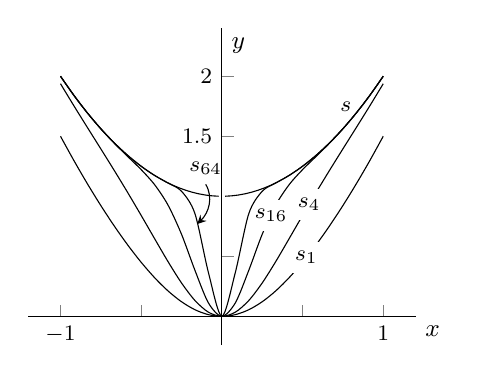
\begin{tikzpicture}
\begin{axis}[small,axis lines*=middle,ymax=2.4,xtick={-1,-0.5,0,0.5,1},xticklabels={$-1$,,$0$,,$1$},ytick={0.5,1.5,2},yticklabels={,$1.5$,$2$},xlabel={$x$},ylabel={$y$},xlabel style={at={(current axis.right of origin)},anchor=north west},ylabel style={rotate=-90},ylabel style={at={(current axis.above origin)},anchor=north west}]
\addplot[domain=-1:1,smooth] {1+x^2-1/(1+x^2)^16}node[pos=0.7,fill=white,font=\footnotesize]{$s_{16}$};
\addplot[domain=-1:1,smooth] {1+x^2-1/(1+x^2)^1}node[pos=0.7,fill=white,font=\footnotesize]{$s_1$};
\addplot[domain=-1:1,smooth] {1+x^2-1/(1+x^2)^4}node[pos=0.75,fill=white,font=\footnotesize]{$s_4$};
\addplot[domain=-1:1,smooth] {1+x^2-1/(1+x^2)^64}coordinate[pos=0.33](kA);
\addplot[domain=0.02:1] {1+x^2}node[pos=0.8,left,font=\footnotesize]{$s$};
\addplot[domain=-1:-0.02] {1+x^2};
\draw[stealth-] (kA) to [out=45,in=-60](axis cs:-0.1,1.1)node[above,font=\footnotesize]{$s_{64}$};
\end{axis}
\end{tikzpicture}
\caption{مثال \حوالہ{مثال_ٹیلر_عجیب_تسلسل} کے چند جزوی مجموعے}
\label{شکل_مثال_ٹیلر_عجیب_تسلسل}
\end{figure}
\انتہا{مثال}
%==========================
اس مثال میں تسلسل کی صورت درج ذیل ہے۔
\begin{align}\label{مساوات_ٹیلر_عمومی_اجزاء_الف}
\sum\limits_{n=0}^{\infty} f_n(z)=f_0(z)+f_1(z)+f_2(z)+\cdots
\end{align}
ہم فرض کرتے ہیں کہ خطہ \عددی{G} میں تمام \عددی{z} کے لئے مساوات \حوالہ{مساوات_ٹیلر_عمومی_اجزاء_الف} مرتکز ہے۔فرض کریں کہ مساوات \حوالہ{مساوات_ٹیلر_عمومی_اجزاء_الف} کا مجموعہ \عددی{s(z)} اور اس کا \عددی{n} واں جزوی مجموعہ \عددی{s_n(z)} ہے۔ہم جانتے ہیں کہ نقطہ \عددی{z} پر مرکوزیت کا مطلب ہے کہ دیے گئے \عددی{ \epsilon >0} کے لئے ہم ایسا \عددی{N=N(\epsilon)} تلاش کر سکتے ہیں کہ درج ذیل مساوات تمام \عددی{n>N(\epsilon,z)} کے لئے مطمئن ہو گا۔
\begin{align*}
\abs{s(z)-s_n(z)}<\epsilon\quad \quad \quad n>N(\epsilon,z)
\end{align*}
\عددی{N} کی قیمت \عددی{\epsilon} پر اور عموماً زیر بحث منتخب نقطہ \عددی{z} پر منحصر ہو گی۔اب کسی دیے گئے \عددی{\epsilon>0} کی صورت میں عین ممکن ہے کہ ہم \عددی{z} \ترچھا{کا غیر تابع} ایسا \عددی{N(\epsilon)} تلاش کر سکیں کہ \عددی{G} میں تمام \عددی{z} کے لئے اور \عددی{n>N(\epsilon)} کے لئے  درج ذیل مطمئن ہو۔
\begin{align*}
\abs{s(z)-s_n(z)}<\epsilon\quad \quad \quad n>N(\epsilon),\quad z\,\,\text{تمام}
\end{align*}
تب ہم کہتے ہیں کہ \عددی{G} میں تسلسل \اصطلاح{یکساں مرتکز}\فرہنگ{مرتکز!یکساں}\حاشیہب{uniform convergent}\فرہنگ{convergent!uniform} ہے۔

یوں یکساں ارتکاز ایسی خاصیت ہے جو \عددی{z} کے لامتناہی سلسلہ سے وابستہ ہے جبکہ تسلسل کی ارتکاز \عددی{z} کی مختلف مخصوص قیمتوں کے ساتھ وابستہ ہے جس کا \عددی{z} کی دیگر قیمتوں کے ساتھ کوئی تعلق نہیں ہو گا۔
 
مثال \حوالہ{مثال_ٹیلر_قوت_نمائی_جدول} میں وقفہ \عددی{0\le x\le 1} (بلکہ کسی بھی محدود وقفہ) پر تسلسل یکساں مرتکز ہے۔مثال \حوالہ{مثال_ٹیلر_عجیب_تسلسل} میں تسلسل ایسے کسی بھی وقفہ میں یکساں مرتکز نہیں ہے  جس میں نقطہ \عددی{0} شامل ہو۔اس سے ظاہر ہے کہ حتمی مرتکز تسلسل بھی غیر یکساں مرتکز ہو سکتا ہے۔اسی طرح ضروری نہیں ہے کہ ایک یکساں مرتکز تسلسل، حتمی مرتکز بھی ہو۔درج ذیل مثال میں ایسی صورت پیش کی گئی ہے۔

%=====================
\ابتدا{مثال}\quad \موٹا{یکساں لیکن غیر حتمی مرتکز تسلسل}\\
درج ذیل تسلسل
\begin{align*}
\sum\limits_{n=1}^{\infty} \frac{(-1)^{n-1}}{x^2+n}=\frac{1}{x^2+1}-\frac{1}{x^2+2}+\frac{1}{x^2+3}-+\cdots\quad \quad (x\,\,\text{حقیقی})
\end{align*}
تمام حقیقی \عددی{x} کے  لئے یکساں مرتکز ہے لیکن یہ تسلسل حتمی مرتکز نہیں ہے (سوال \حوالہ{سوال_ٹیلر_جزو_در_جزو_تکمل_نا_ممکن_ثبوت})۔
\انتہا{مثال}
%===========================

عموماً طاقتی تسلسل مثال \حوالہ{مثال_ٹیلر_ہندسی_تسلسل_باقی} کی طرز کے ہوں گے جن کی صورت حال بہت سادہ ہو گا (درج ذیل مسئلہ دیکھیں)۔  

%=========================
\ابتدا{مسئلہ}\شناخت{مسئلہ_ٹیلر_طاقتی_تسلسل_قرص_میں_یکساں_مرتکز}\quad \موٹا{طاقتی تسلسل}\\
غیر صفر رداس ارتکاز \عددی{R} والا طاقتی تسلسل
\begin{align}\label{مساوات_ٹیلر_یکساں_مرکوزیت_ثبوت_الف}
\sum\limits_{n=0}^{\infty} c_n(z-a)^n
\end{align}
رداس \عددی{r<R} کے ہر دائری قرص \عددی{\abs{z-a}\le r} میں یکساں مرتکز ہو گا۔ 
\انتہا{مسئلہ}
%==========================
\ابتدا{ثبوت}\quad
\عددی{\abs{z-a}\le r} کے لئے
\begin{align}\label{مساوات_ٹیلر_یکساں_مرکوزیت_ثبوت_ب}
\abs{c_{n+1}(z-a)^{n+1}+\cdots+c_{n+p}z^{n+p}}\le \abs{c_{n+1}}r^{n+1}+\cdots+\abs{c_{n+p}}r^{n+p}
\end{align}
ہو گا۔چونکہ  \عددی{\abs{z-a}=r<R} کے لئے مساوات \حوالہ{مساوات_ٹیلر_یکساں_مرکوزیت_ثبوت_الف} حتمی مرتکز ہے لہٰذا کوشی اصول مرکوزیت (حصہ \حوالہ{حصہ_ترتیب_کوشی_اصول_مرکوزیت_ترتیب_تسلسل}) کے تحت دیے گئے \عددی{\epsilon>0} کے لئے ہم ایسا \عددی{N(\epsilon)} تلاش کر سکتے ہیں کہ \عددی{p=1,2,\cdots} اور \عددی{n>N(\epsilon)} کے لئے  درج ذیل مطمئن ہو۔
\begin{align*}
\abs{c_{n+1}}r^{n+1}+\cdots+\abs{c_{n+p}}r^{n+p}<\epsilon
\end{align*}
اس سے اور مساوات \حوالہ{مساوات_ٹیلر_یکساں_مرکوزیت_ثبوت_ب} سے ہر \عددی{p=1,2,\cdots}، ہر \عددی{n>N(\epsilon)} اور قرص \عددی{\abs{z-a}\le r} میں ہر \عددی{z} کے لئے درج ذیل حاصل ہوتا ہے۔
\begin{align*}
\abs{c_{n+1}(z-a)^{n+1}+\cdots+c_{n+p}(z-a)^{n+p}}<\epsilon
\end{align*}
\عددی{N(\epsilon)} کی قیمت \عددی{z} کے غیر تابع ہے جو یکساں مرکوزیت کی نشانی ہے اور یوں مسئلے کا ثبوت مکمل ہوتا ہے۔
\انتہا{ثبوت}
%==============================

اگرچہ متناہی تعداد کے استمراری تفاعل کا مجموعہ استمراری ہو گا البتہ جیسا ہم نے مثال \حوالہ{مثال_ٹیلر_عجیب_تسلسل} میں دیکھا، اگر لامتناہی تعداد کی استمراری تفاعل کا مجموعہ حتمی مرتکز ہو تب بھی اس کا مجموعہ  غیر استمراری ہو سکتا ہے۔اس کے برعکس اگر ایک تسلسل یکساں مرتکز ہو تب ایسا نہیں ہو گا۔درج ذیل مسئلہ اسی حقیقت کو بیان کرتا ہے۔

%==========================
\ابتدا{مسئلہ}\شناخت{مسئلہ_ٹیلر_استمراری_تفاعل}\quad \موٹا{استمرار}\\
فرض کریں کہ تسلسل
\begin{align*}
\sum\limits_{m=0}^{\infty} f_m(z)=f_0(z)+f_1(z)+\cdots
\end{align*}
خطہ \عددی{G} میں یکساں مرتکز ہے اور اس کا مجموعہ \عددی{F(z)} ہے۔تب اگر \عددی{G} میں نقطہ \عددی{z_0} پر ہر جزو \عددی{f_m(z)} استمراری ہو تب \عددی{z_0} پر تفاعل  \عددی{F(z)} استمراری ہو گا۔
\انتہا{مسئلہ}
%=========================== 
\ابتدا{ثبوت}\quad
فرض کریں کہ تسلسل کا \عددی{n} واں جزوی مجموعہ \عددی{s_n(z)} اور مطابقتی باقی \عددی{R_n(z)} ہے:
\begin{align*}
s_n=f_0+f_1+\cdots+f_n,\quad R_n=f_{n+1}+f_{n+2}+\cdots
\end{align*}
چونکہ تسلسل یکساں مرتکز ہے، دیے گئے \عددی{\epsilon>0} کے لئے ہم ایسا \عددی{n=n(\epsilon)} تلاش کر سکتے ہیں کہ \عددی{G} میں تمام \عددی{z} کے لئے درج ذیل مطمئن ہو۔
\begin{align*}
\abs{R_N(z)}<\frac{\epsilon}{3}\quad \quad \quad (\text{\RL{$\,G\,$ میں تمام $\,z\,$}})
\end{align*}
چونکہ \عددی{s_N(z)} نقطہ \عددی{z_0} پر استمراری تفاعل کی متناہی تعداد  کا مجموعہ ہے لہٰذا \عددی{z_0} پر یہ استمراری ہو گا۔یوں ہم ایسا \عددی{\sigma} تلاش کر سکتے ہیں کہ  \عددی{G} میں ان تمام \عددی{z} کے لئے جن کے لئے \عددی{\abs{z-z_0}<\sigma} ہو درج ذیل مطمئن ہو گا۔
\begin{align*}
\abs{s_N(z)-s_N(z_0)}<\frac{\epsilon}{3}\quad \quad \quad (\abs{z-z_0}<\sigma, \quad \text{\RL{$\,G\,$میں تمام $\,z\,$}})
\end{align*}
تکونی عدم مساوات (حصہ \حوالہ{حصہ_مخلوط_قطبی_صورت_عدم_مساوات}) کی مدد سے ان \عددی{z} کے لئے
\begin{align*}
\abs{F(z)-F(z_0)}&=\abs{s_N(z)+R_N(z)-[s_N(z_0)+R_N(z_0)]}\\
&\le \abs{s_N(z)-s_N(z_0)}+\abs{R_N(z)}+\abs{R_N(z_0)}<\frac{\epsilon}{3}+\frac{\epsilon}{3}+\frac{\epsilon}{3}=\epsilon
\end{align*}
لکھا جا سکتا ہے جس سے مراد \عددی{z_0} پر \عددی{F(z)} کی استمرار ہے۔یوں ثبوت مکمل ہوتا ہے۔
\انتہا{ثبوت}
%======================

اس مسئلے میں یکساں مرکوزیت کی شرط  کافی ہے  نا کہ لازمی۔درج ذیل مثال اس حقیقت کی وضاحت کرتی ہے۔

%======================
\ابتدا{مثال}\quad
فرض کریں کہ
\begin{align*}
u_m(x)=\frac{mx}{1+m^2x^2}, \quad f_m(x)=u_m(x)-u_{m-1}(x)
\end{align*}
ہے۔ہم  تسلسل
\begin{align*}
\sum\limits_{m=1}^{\infty} f_m(x)
\end{align*}
پر غور کرتے ہیں۔ اس تسلسل کا \عددی{n} واں جزوی مجموعہ
\begin{align*}
s_n=u_1-u_0+u_2-u_1+\cdots+u_n-u_{n-1}=u_n-u_0=u_n
\end{align*}
ہو گا۔یوں اس کا مجموعہ 
\begin{align*}
F(x)=\lim_{n\to \infty} s_n(x)=\lim_{n\to \infty} u_n(x)=0
\end{align*}
ہو گا جو استمراری تفاعل ہے۔البتہ یہ تسلسل وقفہ \عددی{0\le x\le a} میں یکساں مرتکز نہیں ہے جہاں \عددی{a>0} ہے۔در حقیقت 
\begin{align*}
\abs{F(x)-s_n(x)}=\frac{nx}{1+n^2x^2}<\epsilon
\end{align*} 
سے ہمیں 
\begin{align*}
\frac{nx}{\epsilon}<1+n^2x^2 \quad \implies \quad n^2x^2-\frac{nx}{\epsilon}+1>0
\end{align*}
ملتا ہے جس سے
\begin{align*}
n>\frac{1}{2x\epsilon}(1+\sqrt{1-4\epsilon^2})
\end{align*}
حاصل ہوتا ہے۔مقررہ \عددی{\epsilon} کے لئے \عددی{x\to 0} کرنے سے دایاں ہاتھ لامتناہی تک پہنچتا ہے جس سے ظاہر ہے کہ اس وقفہ میں تسلسل یکساں مرتکز نہیں ہے۔
\انتہا{مثال}
%===============================
ہم کس صورت میں تسلسل کا جزو در جزو تکمل لے سکتے ہیں؟

ہم ایک ایسی مثال  پیش کرتے ہیں جس کا جزو در جزو تکمل لینا  ممکن نہیں ہے۔ 

%===========================
\ابتدا{مثال}\شناخت{مثال_ٹیلر_جزو_در_جزو_تکمل_نا_ممکن}\quad \موٹا{ایسا تسلسل جس کا جزو در جزو تکمل ممکن نہیں ہے}\\
تفاعل
\begin{align*}
u_m(x)=mxe^{-mx^2}, \quad f_m(x)=u_m(x)-u_{m-1}(x)
\end{align*}
پر مبنی تسلسل
\begin{align*}
\sum\limits_{m=1}^{\infty} f_m(x)
\end{align*}
پر وقفہ \عددی{0\le x\le 1} میں غور کرتے ہیں۔اس تسلسل کا \عددی{n} واں جزوی مجموعہ درج ذیل ہو گا۔
\begin{align*}
s_n=u_1-u_0+u_2-u_1+\cdots+u_n-u_{n-1}=u_n-u_0=u_n
\end{align*}
اس طرح اس تسلسل کا مجموعہ
\begin{align*}
F(x)=\lim_{n\to \infty} s_n(x)=\lim_{n\to \infty} u_n(x)=0\quad \quad \quad (0\le x\le 1)
\end{align*}
ہو گا جس سے
\begin{align*}
\int_0^1 F(x)\dif x=0
\end{align*}
حاصل ہوتا ہے۔اس کے برعکس تسلسل کا جزو در جزو تکمل لینے سے درج ذیل ملتا ہے۔
\begin{align*}
\sum\limits_{m=1}^{\infty} \int_0^1 f_m(x)\dif x=\lim_{n\to \infty} \sum\limits_{m=1}^{n}\int_0^1 f_m(x)\dif x=\lim_{n\to \infty} \int_0^1 s_n(x)\dif x
\end{align*}
اب \عددی{s_n=u_n}  ہے لہٰذا دایاں ہاتھ 
\begin{align*}
\lim_{n\to \infty} \int_0^1 u_n(x)\dif x=\lim_{n\to \infty}\int_0^1 nxe^{-nx^2}\dif x=\lim_{n\to \infty} \frac{1}{2}(1-e^{-n})=\frac{1}{2}
\end{align*}
دیتا ہے نا کہ صفر۔اس سے ظاہر ہوتا ہے کہ اس تسلسل کا \عددی{x=0} تا \عددی{x=1} جزو در جزو تکمل حاصل نہیں کیا جا سکتا ہے۔ 
\انتہا{مثال}
%=====================================

مثال \حوالہ{مثال_ٹیلر_جزو_در_جزو_تکمل_نا_ممکن} میں تسلسل دیے گئے وقفہ پر یکساں مرتکز نہیں ہے۔ہم اب دیکھیں گے کہ استمراری تفاعل پر مبنی یکساں مرتکز تسلسل کا جزو در جزو تکمل حاصل کرنا ممکن ہو گا۔

%===========================
\ابتدا{مسئلہ}\شناخت{مسئلہ_ٹیلر_جزو_در_جزو_قابل_تکمل_تسلسل}\quad \موٹا{جزو در جزو تکمل}\\
فرض کریں کہ
\begin{align*}
F(z)=\sum\limits_{n=0}^{\infty} f_n(z)=f_0(z)+f_1(z)+\cdots
\end{align*}
خطہ \عددی{G} میں استمراری تفاعل کا یکساں مرتکز تسلسل ہے۔فرض کریں کہ \عددی{G} میں \عددی{C} کوئی راہ ہے۔ تب تسلسل
\begin{align}\label{مساوات_ٹیلر_جزو_در_جزو_قابل_تکمل_تسلسل}
\sum\limits_{n=0}^{\infty} \int_C f_n(z)\dif z=\int_C f_0(z)\dif z+\int_Cf_1(z)\dif z+\cdots
\end{align}
مرتکز ہو گا اور اس کا مجموعہ \عددی{\int_C F(z)\dif z} ہو گا۔
\انتہا{مسئلہ}
%===========================
\ابتدا{ثبوت}\quad
مسئلہ \حوالہ{مسئلہ_ٹیلر_استمراری_تفاعل} کے تحت \عددی{F(z)} استمراری ہے۔فرض کریں کہ اس تسلسل کا \عددی{n} واں جزوی مجموعہ \عددی{s_n(z)} اور مطابقتی باقی \عددی{R_n(z)} ہے۔تب \عددی{F=s_n+R_n} لہٰذا
\begin{align*}
\int_CF(z)\dif z=\int_C s_n(z)\dif z+\int_C R_n(z)\dif z
\end{align*}
ہو گا۔فرض کریں کہ \عددی{C} کی لمبائی \عددی{l} ہے۔چونکہ دیا گیا تسلسل یکساں مرتکز ہے، ہر دیے گئے \عددی{\epsilon>0} کے لئے ہم ایسا \عددی{N} تلاش کر سکتے ہیں کہ تمام \عددی{n>N} اور \عددی{G} میں تمام \عددی{z} کے لئے درج ذیل مطمئن ہو۔
\begin{align*}
\abs{R_n(z)}<\frac{\epsilon}{l}\quad \quad \quad (n>N, \text{\RL{$\,G\,$ میں تمام $\,z\,$}})
\end{align*} 
مساوات \حوالہ{مساوات_مخلوط_تکمل_حتمی_قیمت_تخمینہ} کی اطلاق سے تمام \عددی{n>N} کے لئے درج ذیل حاصل ہو گا۔
\begin{align*}
\abs{\int_C R_n(z)\dif z}<\frac{\epsilon}{l}l=\epsilon \quad \quad \quad (n>N)
\end{align*}
چونکہ \عددی{R_n=F-s_n} ہے لہٰذا تمام \عددی{n>N} کے لئے اس سے مراد 
\begin{align*}
\abs{\int_C F(z)\dif z-\int_C s_n(z)\dif z}<\epsilon\quad \quad \quad (n>N)
\end{align*}
ہے۔یوں مساوات \حوالہ{مساوات_ٹیلر_جزو_در_جزو_قابل_تکمل_تسلسل} میں دیا گیا تسلسل مرتکز ہو گا اور اس کا مجموعہ وہی ہو گا جو مسئلہ میں دیا گیا ہے۔
\انتہا{ثبوت}
%==========================
 مسئلہ \حوالہ{مسئلہ_ٹیلر_استمراری_تفاعل} اور مسئلہ \حوالہ{مسئلہ_ٹیلر_جزو_در_جزو_قابل_تکمل_تسلسل} یکساں مرتکز تسلسل کے دو اہم ترین خواص پیش کرتے ہیں۔

چونکہ تکمل اور تفرق آپس میں الٹ اعمال ہیں ہم مسئلہ \حوالہ{مسئلہ_ٹیلر_جزو_در_جزو_قابل_تکمل_تسلسل} سے اخذ کر سکتے ہیں کہ مرتکز تسلسل کا جزو در جزو تفرق لینا ممکن ہو گا پس دیے گئے تسلسل کے اجزاء کی تفرق استمراری ہوں اور حاصل تسلسل یکساں مرتکز ہو۔درج ذیل مسئلہ اس کو بہتر بیان کرتا ہے۔

%===================
\ابتدا{مسئلہ}\شناخت{مسئلہ_ٹیلر_جزو_در_جزو_تفرق_ممکن}\quad \موٹا{جزو در جزو تفرق}\\
فرض کریں کہ تسلسل \عددی{f_0(z)+f_1(z)+f_2(z)+\cdots} خطہ \عددی{G} میں مرتکز ہے اور اس تسلسل کا مجموعہ \عددی{F(z)} ہے۔فرض کریں کہ تسلسل
 \عددی{f'_0(z)+f'_1(z)+f'_2(z)+\cdots} خطہ \عددی{G} میں یکساں مرتکز ہے اور اس کے اجزاء \عددی{f'_0(z)}، \عددی{f'_1(z)}، \نقطے خطہ \عددی{G} میں استمراری ہیں تب \عددی{G} میں تمام \عددی{z} کے لئے 
\begin{align*}
F'(z)=f'_0(z)+f'_1(z)+f'_2(z)+\cdots\quad \quad \quad \text{\RL{($\,G\,$ میں تمام $\,z\,$)}}
\end{align*}
ہو گا۔
\انتہا{مسئلہ}
%===========================
اس مسئلہ کا سادہ ثبوت آپ سے سوال \حوالہ{سوال_ٹیلر_جزو_دو_جزو_تفرق_بذریعہ_جزو_در_جزو_تکمل} میں مانگا گیا ہے۔

عموماً یکساں ارتکاز کو تقابلی آزمائش کے ذریعہ  پرکھا جاتا ہے جس کو وائشسٹراس کی آزمائش \عددی{M} کہتے ہیں۔

%===================
\ابتدا{مسئلہ}\شناخت{مسئلہ_ٹیلر_وائشسٹراس_آزمائش_ایم}\quad \موٹا{وائشسٹراس آزمائش \عددی{M}}\\
اگر خطہ \عددی{G} میں تمام \عددی{z} کے لئے مساوات \حوالہ{مساوات_ٹیلر_عمومی_اجزاء_الف} کی طرز کے تسلسل کی اجزاء کی حتمی قیمتیں بالترتیب مستقل اجزاء کی مرتکز تسلسل
\begin{align}
M_0+M_1+M_2+\cdots
\end{align} 
کے اجزاء کے برابر  یا ان سے کم ہو تب یہ تسلسل (مساوات \حوالہ{مساوات_ٹیلر_عمومی_اجزاء_الف}) خطہ\عددی{G} میں یکساں مرتکز ہو گا۔ 
\انتہا{مسئلہ}
%=======================
اس مسئلے کا سادہ ثبوت آپ سے سوال \حوالہ{سوال_ٹیلر_ثبوت_آزمائش_ائشسٹراس_ایم} میں مانگا گیا ہے۔

%===============
\ابتدا{مثال}\quad \موٹا{وائشسٹراس آزمائش \عددی{M}}\\
تسلسل
\begin{align}\label{مساوات_ٹیلر_وائشسٹراس_ایم}
\sum\limits_{m=1}^{\infty} \frac{\sin mx}{m^2}\quad \quad \quad (x\,\text{حقیقق})
\end{align}
پر غور کرتے ہیں۔ چونکہ
\begin{align*}
\abs{\frac{\sin mx}{m^2}}\le \frac{1}{m^2}
\end{align*}
 اور \عددی{\sum \tfrac{1}{m^2}} مرتکز (مساوات \حوالہ{مساوات_ترتیب_تسلسل_مربع_بالعکس}) ہے  لہٰذا  وائشسٹراس آزمائش \عددی{M} کے تحت  ہر وقفہ پر مساوات \حوالہ{مساوات_ٹیلر_وائشسٹراس_ایم} میں دیا گیا تسلسل یکساں مرتکز  ہو گا۔
\انتہا{مثال}
%========================

\حصہء{سوالات}
سوال \حوالہ{سوال_ٹیلر_یکساں_ارتکاز_الف} تا سوال \حوالہ{سوال_ٹیلر_یکساں_ارتکاز_ب} میں ثابت کریں کہ دیا گیا تسلسل دیے گئے خطے میں یکساں مرتکز ہے۔

%===============
\ابتدا{سوال}\شناخت{سوال_ٹیلر_یکساں_ارتکاز_الف}\quad
$\sum\limits_{n=0}^{\infty}z^n,\quad \abs{z}\le 0.99$\\
جواب:\quad مسئلہ \حوالہ{مسئلہ_ٹیلر_طاقتی_تسلسل_قرص_میں_یکساں_مرتکز} سے اخذ ہوتا ہے۔
\انتہا{سوال}
%==================
\ابتدا{سوال}\quad
$\sum\limits_{n=0}^{\infty}\frac{z^n}{n!},\quad \abs{z}\le 10^{30}$
\انتہا{سوال}
%===================
\ابتدا{سوال}\quad
$\sum\limits_{n=1}^{\infty}\frac{(n!)^2}{(2n)!}z^n,\quad \abs{z}\le 3.9$\\
جواب:\quad
چونکہ رداس ارتکاز \عددی{4} ہے لہٰذا مسئلہ \حوالہ{مسئلہ_ٹیلر_طاقتی_تسلسل_قرص_میں_یکساں_مرتکز} سے اخذ ہوتا ہے۔
\انتہا{سوال}
%===================
\ابتدا{سوال}\quad
$\sum\limits_{n=1}^{\infty}\frac{z^n}{n^2},\quad \abs{z}\le 1$\\
\انتہا{سوال}
%===================
\ابتدا{سوال}\quad
$\sum\limits_{n=1}^{\infty}\frac{\sin n\abs{z}}{2^n},\quad z\, \text{تمام}$\\
جواب:\quad
\عددی{\abs{\sin n\abs{z}}\le 1} ہے اور \عددی{\sum \tfrac{1}{2^n}} مرتکز ہے۔یوں مسئلہ \حوالہ{مسئلہ_ٹیلر_وائشسٹراس_آزمائش_ایم} سے اخذ ہو گا۔
\انتہا{سوال}
%===================
\ابتدا{سوال}\quad
$\sum\limits_{n=1}^{\infty}\frac{\tanh^n x}{n(n+1)},\quad x\, \text{\RL{تمام حقیقی}}$
\انتہا{سوال}
%===================
\ابتدا{سوال}\quad
$\sum\limits_{n=1}^{\infty}\frac{\cos^n \abs{z}}{n^2},\quad z\, \text{\RL{تمام}}$\\
جواب:\quad
\عددی{\abs{\cos^n\abs{z}}\le 1} ہے اور \عددی{\sum \tfrac{1}{2^n}} مرتکز ہے۔
\انتہا{سوال}
%===================
\ابتدا{سوال}\شناخت{سوال_ٹیلر_یکساں_ارتکاز_ب}\quad
$\sum\limits_{n=1}^{\infty}\frac{1}{\abs{z}+n^2},\quad z\, \text{\RL{تمام}}$
\انتہا{سوال}
%===================
\ابتدا{سوال}\quad
اگر مساوات \حوالہ{مساوات_ٹیلر_عمومی_اجزاء_الف} میں دیا گیا تسلسل خطہ \عددی{G} میں یکساں مرتکز ہو تب دکھائیں کہ یہ \عددی{G} کے کسی بھی حصے میں یکساں مرتکز ہو گا۔ 
\انتہا{سوال}
%=======================
\ابتدا{سوال}\شناخت{سوال_ٹیلر_جزو_دو_جزو_تفرق_بذریعہ_جزو_در_جزو_تکمل}\quad
مسئلہ \حوالہ{مسئلہ_ٹیلر_جزو_در_جزو_تفرق_ممکن} کا مسئلہ \حوالہ{مسئلہ_ٹیلر_جزو_در_جزو_قابل_تکمل_تسلسل} سے اخذ کریں۔
\انتہا{سوال}
%=====================
\ابتدا{سوال}\شناخت{سوال_ٹیلر_ثبوت_آزمائش_ائشسٹراس_ایم}
مسئلہ \حوالہ{مسئلہ_ٹیلر_وائشسٹراس_آزمائش_ایم} کا ثبوت پیش کریں۔
\انتہا{سوال}
%=======================
\ابتدا{سوال}\quad
ایسا چھوٹے سے چھوٹا عدد صحیح \عددی{n} تلاش کریں کہ \عددی{z=x=0.5,0.6,0.7,0.8,0.9} کے لئے مثال \حوالہ{مثال_ٹیلر_ہندسی_تسلسل_باقی} میں  \عددی{\abs{R_n}<0.01} ہو۔ہندسی تسلسل کا مجموعہ \عددی{\tfrac{1}{1-x}} جس میں خلل \عددی{0.01} سے کم ہو حاصل کرنے کی نقطہ نظر سے اس نتیجے کا کیا مطلب ہے۔
\انتہا{سوال}
%=====================
\ابتدا{سوال}\quad
ایسا تسلسل تلاش کریں جس کا \عددی{n} واں جزوی مجموعہ \عددی{s_n(x)=\tfrac{nx}{nx+1}} ہو۔ \عددی{s_1}، \عددی{s_2}، \عددی{s_3}، \عددی{s_4} اور  تمام \عددی{x\ge 0} کے لئے 
$\,s=\lim\limits_{n\to \infty} s_n\,$
 ترسیم کریں۔\\

جواب:\quad
$f_n=s_n-s_{n-1}=\frac{x}{nx+1}[(n-1)x+1]$
\انتہا{سوال}
%======================
\ابتدا{سوال}\quad
ثابت کریں کہ ایسے کسی بھی  وقفہ میں جس میں نقطہ \عددی{x=0} شامل ہو، مثال \حوالہ{مثال_ٹیلر_عجیب_تسلسل} کا تسلسل یکساں مرتکز نہیں ہو گا۔ 
\انتہا{سوال}
%======================
\ابتدا{سوال}\quad
دکھائیں کہ  \عددی{x\ne 0} کے لئے 
$\,x^2\sum\limits_{n=1}^{\infty} \tfrac{1}{(1+x^2)^n}=1\,$
ہے جبکہ \عددی{x=0} کے لئے یہ \عددی{0} کے برابر ہے۔ شکل \حوالہ{شکل_مثال_ٹیلر_عجیب_تسلسل} کی طرح چند جزوی مجموعوں کو ترسیم کریں۔
\انتہا{سوال}
%==========================
\ابتدا{سوال}\quad
مثال \حوالہ{مثال_ٹیلر_عجیب_تسلسل} میں دیے تسلسل میں \عددی{x} کی جگہ \عددی{z} پر کرتے ہوئے اس کی  ارتکاز کا خطہ ٹھیک ٹھیک تلاش کریں۔
\انتہا{سوال}
%=======================
\ابتدا{سوال}\quad
دکھائیں کہ وقفہ \عددی{0\le x\le 1} میں 
$\,1+\sum\limits_{n=1}^{\infty} (x^n-x^{n-1})\,$
یکساں استمراری نہیں ہے۔جزوی مجموعہ \عددی{s_1}، \عددی{s_2}، \عددی{s_3} اور \عددی{s_4} ترسیم کریں۔
\انتہا{سوال}
%========================
\ابتدا{سوال}\شناخت{سوال_ٹیلر_جزو_در_جزو_تکمل_نا_ممکن_ثبوت}\quad
مثال \حوالہ{مثال_ٹیلر_جزو_در_جزو_تکمل_نا_ممکن} میں دیا گیا فقرہ ثابت کریں۔
\انتہا{سوال}
%======================
\موٹا{حراری مساوات}: دکھائیں کہ مساوات \حوالہ{مساوات_جزوی_حل_حرارت_ج} جس کے عددی سر مساوات \حوالہ{مساوات_جزوی_حل_حرارت_چ} دیتی ہے، حراری مساوات کا  \عددی{t>0} کے لئے حل ہے جہاں وقفہ \عددی{0\le x\le l} پر \عددی{f(x)} استمراری فرض کیا گیا ہے اور اس وقفہ کے اندر اس کے تمام یک طرفہ تفرق پائے جاتے ہیں۔ یہ ثابت کرنے کی خاطر درج ذیل کرنا ہو گا۔

%=================
\ابتدا{سوال}\شناخت{سوال_ٹیلر_حراری_الف}\quad
دکھائیں کہ \عددی{\abs{B_n}} محدود ہے مثلاً تمام \عددی{n} کے لئے \عددی{\abs{B_n}<K} ہے۔اس سے  درج ذیل اخذ کریں۔ 
\begin{align*}
\abs{u_n}<K e^{-\lambda_n^2 t_0}\quad \quad \quad (t\ge t_0 >0)
\end{align*}
یوں وائشسٹراس آزمائش \عددی{M} کے تحت  \عددی{x} اور \عددی{t} کے لحاظ سے \عددی{t\ge t_0} اور \عددی{0\le x\le l} کی صورت میں مساوات \حوالہ{مساوات_جزوی_حل_حرارت_ج} کا تسلسل یکساں مرتکز ہو گا۔مسئلہ \حوالہ{مسئلہ_ٹیلر_استمراری_تفاعل} استعمال کرتے ہوئے دکھائیں کہ \عددی{t\ge t_0} کی صورت میں \عددی{u(x,t)} استمراری ہو گا  لہٰذا \عددی{t\ge t_0} کے لئے یہ مساوات \حوالہ{مساوات_جزوی_حراری_ب} کی سرحدی شرائط مطمئن کرے گا۔
\انتہا{سوال}
%==========================
\ابتدا{سوال}\شناخت{سوال_ٹیلر_حراری_ب}\quad
دکھائیں کہ \عددی{t\ge t_0} کے لئے
$\,\abs{\frac{\partial u_n}{\partial t}}<\lambda^2_n Ke^{-\lambda^2_n t_0}\,$
ہو گا اور تناسبی آزمائش کے تحت دایاں ہاتھ مرتکز ہو گا۔اس سے، آزمائش وائشسٹراس سے اور مسئلہ \حوالہ{مسئلہ_ٹیلر_جزو_در_جزو_تفرق_ممکن} سے  اخذ کریں کہ مساوات \حوالہ{مساوات_جزوی_حل_حرارت_ج} میں دیا گیا تسلسل \عددی{t} کے لحاظ سے جزو در جزو قابل تفرق ہے جس سے  حاصل تسلسل کا مجموعہ \عددی{\tfrac{\partial u}{\partial t}} ہو گا۔ دکھائیں کہ \عددی{x} کے لحاظ سے مساوات \حوالہ{مساوات_جزوی_حل_حرارت_ج}  دو مرتبہ قابل تفرق ہے جس سے  حاصل تسلسل کا مجموعہ
 \عددی{\tfrac{\partial^{\,2} u}{\partial x^2}} ہو گا۔اس سے اور سوال \حوالہ{سوال_ٹیلر_حراری_الف} سے اخذ کریں کہ تمام \عددی{t\ge t_0} کے لئے مساوات \حوالہ{مساوات_جزوی_حل_حرارت_ج} حراری مساوات کا حل ہے۔(ہم یہاں بغیر ثبوت پیش کئے بتانا چاہتے ہیں کہ مساوات \حوالہ{مساوات_جزوی_حل_حرارت_ج} ابتدائی شرائط کو بھی مطمئن کرتا ہے۔)
\انتہا{سوال}
%=======================

\حصہ{لوغوں تسلسل}\شناخت{حصہ_ٹیلر_لوغوں_تسلسل}
کئی مسائل میں تفاعل \عددی{f(z)} کا تسلسل ایسا نقطوں کے گرد درکار ہو گا جہاں تفاعل نادر ہو گا۔ایسی صورت میں ٹیلر تسلسل قابل استعمال نہیں ہو گی۔ ایک نئی قسم کی تسلسل جسے \ترچھا{لوغوں تسلسل} کہتے ہیں کا استعمال یہاں ضروری ہو گا۔ایسا چھلا جو ہم مرکز دائرہ \عددی{C_1} اور \عددی{C_2} کے درمیان پایا جاتا ہو اور \عددی{f(z)} اس چھلا میں اور \عددی{C_1} اور \عددی{C_2} کے ہر نقطہ پر تحلیلی ہو میں لوغوں تسلسل کارآمد ہو گا (شکل \حوالہ{شکل_ٹیلر_مسئلہ_لوغوں})۔ٹیلر تسلسل کی طرح، یہاں بھی \عددی{f(z)} دائرہ \عددی{C_1} کے باہر چند نقطوں پر نادر ہو سکتا ہے، اور اب لازمی نیا پہلو کے طور پر \عددی{C_2} کے اندر بھی \عددی{f(z)} چند نقطوں پر نادر ہو سکتا ہے۔
\begin{figure}
\centering
\begin{tikzpicture}
\fill[gray!20!white](0,0) circle (1.5);
\fill[white](0,0) circle (0.75);
\draw(0,0) circle (0.75);
\draw(0,0)node[ocirc]{}node[below]{$a$} circle (1.5);
\draw(-30:0.75)node[right]{$C_2$};
\draw(40:1.5) node [right]{$C_1$};
\draw[thick,->-=0.35,rotate around={-25:(-25:0.15)}](-25:0.15) circle (1.2cm and 1cm);
\draw[rotate around={-25:(-25:0.15)}](-25:0.15)++(135:0.9cm and 1.3cm)node[above]{$C$};
\end{tikzpicture}
\caption{مسئلہ لوغوں}
\label{شکل_ٹیلر_مسئلہ_لوغوں}
\end{figure}

%=================
\ابتدا{مسئلہ}\quad \موٹا{مسئلہ لوغوں}\\
اگر دو ہم مرکز دائروں \عددی{C_1} اور \عددی{C_2} جن کا مرکز \عددی{a} ہو پر \عددی{f(z)} تحلیلی ہو اور ان دائروں کے درمیان چھلا میں بھی \عددی{f(z)} تحلیلی ہو تب \عددی{f(z)} کو \اصطلاح{لوغوں تسلسل}\فرہنگ{لوغوں!تسلسل}\فرہنگ{تسلسل!لوغوں}\حاشیہب{Laurent series}\فرہنگ{Laurent!series}\فرہنگ{series!Laurent}
\begin{multline}\label{مساوات_ٹیلر_لوغوں_تسلسل_الف}
f(z)=\sum\limits_{n=0}^{\infty} b_n(z-a)^n+\sum\limits_{n=1}^{\infty}\frac{c_n}{(z-a)^n}\\
=b_0+b_1(z-a)+b_2(z-a)^2+\cdots+\frac{c_1}{z-a}+\frac{c_2}{(z-a)^2}+\cdots
\end{multline}
ظاہر\حاشیہد{فرانسیسی ریاضی دان پیّر الفنس لوغوں [1813-1854]} کر سکتا ہے جہاں عددی سر\حاشیہد{چونکہ \عددی{z} کو \عددی{f(z)} میں استعمال کیا گیا ہے لہٰذا ہم تکمل کے متغیرہ کو \عددی{z^*} لکھتے ہیں۔}
\begin{align}\label{مساوات_ٹیلر_لوغوں_تسلسل_ب}
b_n=\frac{1}{i2\pi}\int_C\frac{f(z^*)}{(z^*-a)^{n+1}}\dif z^*,\quad c_n=\frac{1}{i2\pi}\int_C (z^*-a)^{n-1} f(z^*)\dif z^*
\end{align}
ہیں جہاں تکمل کو، چھلا کے اندر  اور اندرونی دائرے کو گھیرتے ہوئے  کسی بھی سادہ بند راہ \عددی{C} پر گھڑی کی الٹ رخ، حاصل کیا جا سکتا ہے (شکل \حوالہ{شکل_ٹیلر_مسئلہ_لوغوں})۔

یہ تسلسل مرتکز ہے اور \عددی{f(z)} کو اس کھلے چھلا میں ظاہر کرتا ہے جو موجودہ چھلا کے دائرہ  \عددی{C_1} کو مسلسل اتنا بڑھا کر کہ \عددی{f(z)} کا نادر نقطہ آن پہنچے  اور \عددی{C_2} کو مسلسل اتنا گھٹا کر کہ \عددی{f(z)} کا نادر نقطہ آن پہنچے سے حاصل ہوتا ہے۔

ظاہر ہے کہ مساوات \حوالہ{مساوات_ٹیلر_لوغوں_تسلسل_الف} اور مساوات \حوالہ{مساوات_ٹیلر_لوغوں_تسلسل_الف} کی جگہ
\begin{align}\label{مساوات_ٹیلر_لوغوں_تسلسل_الف_الف}
f(z)=\sum\limits_{n=-\infty}^{\infty} A_n(z-a)^n
\end{align}
جہاں
\begin{align}\label{مساوات_ٹیلر_لوغوں_تسلسل_ب_ب}
A_n=\frac{1}{i2\pi}\int_C \frac{f(z^*)}{(z^*-a)^{n+1}}\dif z^*
\end{align}
ہے لکھا جا سکتا ہے۔
\انتہا{مسئلہ}
%====================================
\ابتدا{ثبوت}\quad
فرض کریں کہ دیے گئے چھلا میں \عددی{z} کوئی نقطہ ہے۔تب کوشی کلیہ تکمل (مساوات \حوالہ{مساوات_مخلوط_تکمل_کوشی_کلیہ_تکمل_پ}) کے تحت
\begin{align}\label{مساوات_ٹیلر_لوغوں_تسلسل_پ}
f(z)=\frac{1}{i2\pi}\int\limits_{C_1} \frac{f(z^*)}{z^*-z}\dif z^*-\frac{1}{i2\pi}\int\limits_{C_2}\frac{f(z^*)}{z^*-z}\dif z^*
\end{align}
ہو گا جہاں گھڑی کی الٹ رخ تکمل لیا جائے گا۔ہم حصہ \حوالہ{حصہ_ٹیلر_تسلسل} کی طرح ان تکملات کو تبدیل کرتے ہیں۔چونکہ \عددی{z} دائرہ \عددی{C_1} کے اندر پایا جاتا ہے لہٰذا پہلا تکمل عین حصہ \حوالہ{حصہ_ٹیلر_تسلسل} کے تکمل کی طرح ہے۔حصہ \حوالہ{حصہ_ٹیلر_تسلسل} کی طرح اس کو پھیلا کر باقی کا تخمینہ لگاتے ہوئے
\begin{align}
\frac{1}{i2\pi}\int\limits_{C_1}\frac{f(z^*)}{z^*-z}\dif z^*=\sum\limits_{n=0}^{\infty} b_n(z-a)^n
\end{align}
ملتا ہے جہاں عددی سر درج ذیل کلیہ دیتا ہے جہاں گھڑی کی الٹ رخ تکمل حاصل کیا جاتا ہے۔
\begin{align}
b_n=\frac{1}{i2\pi}\int\limits_{C_1} \frac{f(z^*)}{(z^*-a)^{n+1}}\dif z^*
\end{align}
چونکہ \عددی{a} چھلے کا حصہ نہیں ہے لہٰذا چھلا میں  تفاعل \عددی{\tfrac{f(z^*)}{(z^*-a)^{n+1}}}  تحلیلی ہو گا۔یوں \عددی{b_n} کی قیمت تبدیل کیے بغیر ہم \عددی{C_1} کی جگہ راہ \عددی{C} پر تکمل حاصل کر سکتے ہیں۔یوں تمام \عددی{n\ge 0} کے لئے مساوات \حوالہ{مساوات_ٹیلر_لوغوں_تسلسل_ب} کا ثبوت مکمل ہوتا ہے۔

مساوات \حوالہ{مساوات_ٹیلر_لوغوں_تسلسل_پ} کے دایاں تکمل میں صورت حال مختلف ہے۔چونکہ \عددی{z} دائرہ \عددی{C_2} کے باہر پایا جاتا ہے لہٰذا مساوات \حوالہ{مساوات_ٹیلر_کوشی_کلیہ_تکمل_ٹیلر_پ} کی جگہ اب
\begin{align}\label{مساوات_ٹیلر_اکائی_سے_کم}
\abs{\frac{z^*-a}{z-a}}<1
\end{align}
ہو گا اور ہمیں \عددی{\tfrac{1}{z^*-z}} کو \عددی{\tfrac{z^*-a}{z-a}} کی طاقتوں میں پھیلانا ہو گا تا کہ حاصل تسلسل مرتکز ہو۔یوں 
\begin{align*}
\frac{1}{z^*-z}=\frac{1}{z^*-a-(z-a)}=\frac{-1}{(z-a)\big(1-\frac{z^*-a}{z-a}\big)}
\end{align*}
لکھ کر متناہی ہندسی تسلسل کے کلیہ کو استعمال کرتے ہوئے 
\begin{multline*}
\frac{1}{z^*-z}=-\frac{1}{z-a}\big \{1+\frac{z^*-a}{z-a}+\big(\frac{z^*-a}{z-a}\big)^2 +\cdots+\big(\frac{z^*-a}{z-a}\big)^n\big \}\\
-\frac{1}{z-z^*}\big(\frac{z^*-a}{z-a}\big)^{n+1}
\end{multline*}
حاصل ہوتا ہے۔اس کو \عددی{-\tfrac{f(z^*)}{i2\pi}} سے ضرب دے کر \عددی{C_2} پر تکمل لینے سے مساوات \حوالہ{مساوات_ٹیلر_لوغوں_تسلسل_پ} کا دایاں تکمل حاصل ہو گا یعنی:
\begin{multline*}
-\frac{1}{i2\pi}\int\limits_{C_2} \frac{f(z^*)}{z^*-z}\dif z^*\\
=\frac{1}{i2\pi}\big\{\frac{1}{z-a}\int\limits_{C_2}f(z^*)\dif z^*+\frac{1}{(z-a)^2}\int\limits_{C_2} (z^*-a)f(z^*)\dif z^*+\cdots \\
+\frac{1}{(z-a)^{n+1}}\int\limits_{C_2} (z^*-a)^nf(z^*)\dif z^* \big \}+R^*_n(z)
\end{multline*} 
اس روپ میں آخری جزو درج ذیل ہو گا۔
\begin{align}\label{مساوات_ٹیلر_لوغوں_باقی_الف}
R^*_n(z)=\frac{1}{i2\pi(z-a)^{n+1}}\int\limits_{C_2} \frac{(z^*-a)^{n+1}}{z-z^*}f(z^*)\dif z^*
\end{align}
کنگنی قوسین کے اندر  تکملوں میں \عددی{C_2} کی جگہ راہ \عددی{C} استعمال کی جا سکتی ہے جس سے تکمل کی قیمت تبدیل نہیں ہوتی ہے۔یوں اگر 
\begin{align}\label{مساوات_ٹیلر_لوغوں_باقی_ب}
\lim_{n\to \infty}R^*_n(z) =0
\end{align}
ہو تب مسئلہ لوغوں ثابت ہوتا ہے۔ 

ہم مساوات \حوالہ{مساوات_ٹیلر_لوغوں_باقی_ب} کو ثابت رکتے ہیں۔چونکہ \عددی{z-z^*\ne 0} ہے اس لئے \عددی{C_2} پر اور چھلا میں \عددی{f(z)} تحلیلی ہو گا اور  \عددی{C_2} پر تمام \عددی{z} کے لئے 
$\,\tfrac{f(z^*)}{z-z^*}\,$
کی حتمی قیمت محدود ہو گی مثلاً:
\begin{align*}
\abs{\frac{f(z^*)}{z-z^*}}<\tilde{M}\quad \quad \quad \text{\RL{$\,C_2\,$ پر تمام $\,z\,$}}
\end{align*}
راہ \عددی{C_2} کی لمبائی کو \عددی{l} لیتے ہوئے  مساوات \حوالہ{مساوات_ٹیلر_لوغوں_باقی_الف} پر مساوات \حوالہ{مساوات_مخلوط_تکمل_حتمی_قیمت_تخمینہ} کے اطلاق سے
\begin{align*}
\abs{R^*_n(z)}<\frac{1}{2\pi\abs{z-a}^{n+1}}\abs{z^*-a}^{n+1}\tilde{M} l=\frac{\tilde{M}l}{2\pi}\abs{\frac{z^*-a}{z-a}}^{n+1}
\end{align*}
حاصل ہوتا ہے۔مساوات \حوالہ{مساوات_ٹیلر_اکائی_سے_کم} کی مدد سے ہم دیکھتے ہیں کہ \عددی{n} کی قیمت لامتناہی تک پہنچانے سے درج بالا میں دایاں جزو صفر تک پہنچتا ہے۔یوں مساوات \حوالہ{مساوات_ٹیلر_لوغوں_باقی_ب} ثابت ہوتی ہے لہٰذا دیے گئے چھلا میں مساوات \حوالہ{مساوات_ٹیلر_لوغوں_تسلسل_الف} ثابت ہوتی ہے جس کے عددی سر مساوات \حوالہ{مساوات_ٹیلر_لوغوں_تسلسل_ب} دیتی ہے۔

آخر میں ہم کھلے چھلا میں مساوات \حوالہ{مساوات_ٹیلر_لوغوں_تسلسل_الف} کی ارتکاز ثابت کرتے ہیں۔

ہم مساوات \حوالہ{مساوات_ٹیلر_لوغوں_تسلسل_ب} میں  اجزاء کے مجوعوں کو \عددی{g(z)} اور \عددی{h(z)} لکھتے ہیں، اور \عددی{C_1} اور \عددی{C_2} کے رداس کو بالترتیب \عددی{r_1} اور \عددی{r_2} لکھتے ہیں۔تب \عددی{f=g+h} ہو گا۔ پہلا تسلسل طاقتی تسلسل ہے جو  چھلا میں مرتکز ہے  لہٰذا یہ تسلسل دائرہ \عددی{C_1} کے اندر پورے قرص پر مرتکز ہو گا اور \عددی{g} اس قرص میں تحلیلی ہو گا۔

آخری تسلسل میں \عددی{Z=\tfrac{1}{z-a}} لکھ کر \عددی{Z} کا طاقتی تسلسل حاصل ہوتا ہے اور چھلا \عددی{r_2<\abs{z-a}<r_1} کا مطابقتی چھلا اب
 \عددی{\tfrac{1}{r_1}<\abs{Z}<\tfrac{1}{r_2}} ہو گا۔یہ طاقتی تسلسل اس چھلا میں مرتکز ہے لہٰذا یہ پورے قرص \عددی{\abs{Z}<\tfrac{1}{r_2}} میں مرتکز ہو گا۔چونکہ اس  قرص کا مطابقتی خطہ \عددی{\abs{z-a}>r_2} یعنی \عددی{C_2} کی بیرون ہے لہٰذا \عددی{C_2} کے باہر تمام \عددی{z} کے لئے دیا گیا تسلسل مرتکز ہو گا اور \عددی{h} ان تمام \عددی{z} کے لئے مرتکز ہو گا۔

چونکہ \عددی{f=g+h} ہے لہٰذا \عددی{C_1} کے باہر ان تمام نقطوں پر \عددی{g} نادر ہو گا جن پر \عددی{f} نادر ہے اور \عددی{C_2} کے اندر ان تمام نقطوں پر \عددی{h} نادر ہو گا جن پر \عددی{f} نادر ہے۔نتیجتاً پہلا تسلسل \عددی{a} کے گرد ان تمام \عددی{z} پر مرتکز ہو گا جو  اس دائرے میں پائے جاتے ہوں جس کا مرکز \عددی{a} ہو اور جس کا رداس  \عددی{C_1} کے باہر \عددی{f} کے اس نقطہ نادر جو \عددی{a} کے قریب ترین ہو کا \عددی{a} تک فاصلہ کے برابر ہو۔اسی طرح دوسرا تسلسل \عددی{a} کے گرد ان تمام \عددی{z} پر مرتکز ہو گا جو  اس دائرے کے باہر پائے جاتے ہوں جس کا مرکز \عددی{a} ہو اور جس کا رداس  \عددی{C_2} کے اندر  \عددی{f} کے اس نقطہ نادر جو \عددی{a} سے دور ترین ہو کا \عددی{a} تک فاصلہ کے برابر ہو۔ان دونوں  ارتکاز کے دائرہ کار کا مشترکہ دائرہ کار وہ کھلا چھلا ہو گا جس کا مسئلے کے آخر  میں ذکر کیا گیا ہے۔یوں مسئلے کا ثبوت مکمل ہوتا ہے۔  
\انتہا{ثبوت}
%===================================

یوں اگر \عددی{C_2} کے اندر \عددی{f(z)} تحلیلی ہو تب لوغوں تسلسل  گھٹ کر \عددی{f(z)} کے ٹیلر تسلسل کی صورت اختیار کرے گا جس کا مرکز \عددی{a} ہو گا۔بلکہ ایسی صورت میں آپ مساوات \حوالہ{مساوات_ٹیلر_لوغوں_تسلسل_ب} پر کوشی  کلیہ تکمل کے اطلاق سے دیکھ سکتے ہیں کہ مساوات \حوالہ{مساوات_ٹیلر_لوغوں_تسلسل_الف} میں  \عددی{z-a} کی منفی طاقتوں کے تمام عددی سر صفر ہوں گے۔

مزید اگر \عددی{C_2} میں \عددی{f(z)} کا  واحد نقطہ نادر \عددی{z=a} ہو تب ماسوائے نقطہ \عددی{z=a} کے \عددی{C_1} کے اندر تمام \عددی{z} پر  لوغوں تسلسل (مساوات \حوالہ{مساوات_ٹیلر_لوغوں_تسلسل_الف}) مرتکز ہو گا۔ایسی صورت حال عموماً پائی جاتی ہے لہٰذا یہ خصوصاً  اہم ہے۔اس پر ہم جلد مزید غور کریں گے۔

چھلا ارتکاز کے اندر تفاعل \عددی{f(z)} کا لوغوں تسلسل یکتا ہو گا (سوال \حوالہ{سوال_ٹیلر_لوغوں_یکتا})۔البتہ دو مختلف چھلوں جن کا مرکز ایک ہی ہو میں \عددی{f(z)} کے لوغوں تسلسل مختلف ہو سکتے ہیں (مثال \حوالہ{مثال_ٹیلر_لوغوں_مثال_ب})۔

چونکہ لوغوں تسلسل کے عددی سروں کو عموماً مساوات \حوالہ{مساوات_ٹیلر_لوغوں_تسلسل_ب} سے حاصل نہیں کیا جاتا ہے لہٰذا لوغوں تسلسل کی یکتائی اہم ہے۔لوغوں تسلسل کے حصول کے مختلف طریقے درج ذیل مثالوں میں پیش کیے گئے ہیں۔اگر کسی بھی طریقے  سے کوئی لوغوں تسلسل حاصل کیا جائے تب یقیناً چھلا کے اندر یہی تفاعل کا لوغوں تسلسل ہو گا۔ 

%========================
\ابتدا{مثال}\quad
مساوات \حوالہ{مساوات_ٹیلر_قوت_نمائی_مکلارن_تسلسل} میں \عددی{z} کی جگہ \عددی{\tfrac{1}{z}} پر کرتے ہوئے  تفاعل \عددی{z^2e^{\tfrac{1}{z}}} کا لوغوں تسلسل جس کا مرکز \عددی{0} ہو  حاصل کیا جا سکتا ہے؛
\begin{align*}
z^2e^{\frac{1}{z}}=z^2\big(1+\frac{1}{1!z}+\frac{1}{2!z^2}+\cdots\big)=z^2+z+\frac{1}{2}+\frac{1}{3!z}+\frac{1}{4!z^2}+\cdots\quad \quad (\abs{z}>0)
\end{align*}
\انتہا{مثال}
%=============================
\ابتدا{مثال}\شناخت{مثال_ٹیلر_لوغوں_مثال_ب}\quad \موٹا{مختلف چھلا میں لوغوں تسلسل کا حصول}\\
ہم تفاعل \عددی{f(z)=\tfrac{1}{1-z^2}} کا لوغوں تسلسل تلاش کرتے ہیں جس کا مرکز \عددی{z=1} ہو۔\\
اب \عددی{1-z^2=-(z-1)(z+1)} لکھا جا سکتا ہے۔ہندسی تسلسل
\begin{align*}
\frac{1}{1-q}=\sum\limits_{n=0}^{\infty} q^n\quad \quad \quad (\abs{q}<1)
\end{align*}
استعمال کرتے ہوئے 
\begin{align*}
\text{(الف)}\quad \frac{1}{z+1}&=\frac{1}{2+(z-1)}=\frac{1}{2}\frac{1}{[1-(-\frac{z-1}{2})]}\\
&=\frac{1}{2}\sum\limits_{n=0}^{\infty}\big(-\frac{z-1}{2}\big)^n=\sum\limits_{n=0}^{\infty} \frac{(-1)^n}{2^{n+1}}(z-1)^n
\end{align*}
حاصل ہوتا ہے جو قرص \عددی{\abs{\tfrac{z-1}{2}}<1} یعنی \عددی{\abs{z-1}<2} میں مرتکز ہے (شکل \حوالہ{شکل_مثال_ٹیلر_لوغوں_مثال_ب})۔اسی طرح  تسلسل
\begin{align*}
\text{(ب)}\quad \frac{1}{z+1}&=\frac{1}{(z-1)+2}=\frac{1}{(z-1)}\frac{1}{\big(1+\frac{2}{z-1}\big)}\\
&=\frac{1}{z-1}\sum\limits_{n=0}^{\infty} \big(-\frac{2}{z-1}\big)^n=\sum\limits_{n=0}^{\infty}\frac{(-2)^n}{(z-1)^{n+1}}
\end{align*}
خطہ  \عددی{\abs{\tfrac{2}{z-1}}<1} یعنی \عددی{\abs{z-1}>2} میں مرتکز ہو گا (شکل \حوالہ{شکل_مثال_ٹیلر_لوغوں_مثال_ب})۔یوں (الف) سے  تسلسل
\begin{gather}
\begin{aligned}\label{مساوات_ٹیلر_چھلا_پہلا}
f(z)&=\frac{-1}{(z-1)(z+1)}=\sum\limits_{n=0}^{\infty} \frac{(-1)^{n+1}}{2^{n+1}}(z-1)^{n-1}\\
&=\frac{-\tfrac{1}{2}}{z-1}+\frac{1}{4}-\frac{1}{8}(z-1)+\frac{1}{16}(z-1)^2-+\cdots
\end{aligned}
\end{gather}
حاصل ہو گا جو دائرہ کار \عددی{0<\abs{z-1}<2} میں مرتکز ہے۔اسی طرح (ب) سے تسلسل
\begin{gather}
\begin{aligned}\label{مساوات_ٹیلر_چھلا_دوسرا}
f(z)&=-\sum\limits_{n=0}^{\infty} \frac{(-2)^n}{(z-1)^{n+2}}=-\frac{1}{(z-1)^2}+\frac{2}{(z-1)^3}-\frac{4}{(z-1)^4}+-\cdots
\end{aligned}
\end{gather} 
حاصل ہو گا جو دائرہ کار \عددی{\abs{z-1}>2} میں مرتکز ہے۔
%
\begin{figure}
\centering
\begin{tikzpicture}
\draw(-1.5,0)--(5,0)node[right]{$x$};
\draw(0,-2)--(0,2.5)node[left]{$y$};
\draw[thick](1,0)node[ocirc]{}node[below]{$1$} circle (2);
\draw(-1,0)node[below left]{$-1$}--++(0,0.2);
\draw(1.25,1)node[above]{\RL{لوغوں تسلسل}}node[below]{\RL{مساوات \حوالہ{مساوات_ٹیلر_چھلا_پہلا}}};
\draw(4.25,1)node[above]{\RL{لوغوں تسلسل}}node[below]{\RL{مساوات \حوالہ{مساوات_ٹیلر_چھلا_دوسرا}}};
\end{tikzpicture}
\caption{شکل برائے مثال \حوالہ{مثال_ٹیلر_لوغوں_مثال_ب}}
\label{شکل_مثال_ٹیلر_لوغوں_مثال_ب}
\end{figure}
\انتہا{مثال}
%=======================
\ابتدا{مثال}\quad 
سوال \حوالہ{سوال_ٹیلر_ابتدائی_تین_ب} کے نتیجہ  سے ہم درج ذیل حاصل کرتے ہیں۔
\begin{align*}
\cot z=\frac{1}{z}-\frac{1}{3}z-\frac{1}{45}z^3-\frac{2}{945}z^5-\cdots\quad \quad (0<\abs{z}<\pi)
\end{align*}
\انتہا{مثال}
%=======================
اگر \عددی{C_2} میں  \عددی{f(z)} کا واحد ایک نقطہ نادر \عددی{z=a} ہو (شکل \حوالہ{شکل_ٹیلر_مسئلہ_لوغوں}) تب خطہ
\begin{align}\label{مساوات_ٹیلر_قطب_خطہ}
0<\abs{z-a}<R
\end{align}
میں لوغوں تسلسل (مساوات \حوالہ{مساوات_ٹیلر_لوغوں_تسلسل_الف}) مرتکز ہو گا اور \عددی{z=a} پر \عددی{f(z)} کے نقطہ نادر کو \اصطلاح{قطب}\فرہنگ{قطب}\حاشیہب{pole}\فرہنگ{pole} یا \اصطلاح{لازمی ندرت}\فرہنگ{لازمی ندرت}\حاشیہب{essential singularity}\فرہنگ{singularity!essential} کہتے ہیں۔ اگر لوغوں تسلسل (وہ تسلسل جو \عددی{z=a} کی پڑوس میں مرتکز لیکن عین \عددی{z=a} پر منفرج ہو) میں منفی طاقت  کے متناہی  تعداد کے اجزاء ہوں تب اس نقطہ کو \عددی{قطب} کہتے ہیں اور اگر ان اجزاء کی تعداد لا متناہی ہو تب اس کو \اصطلاح{لازمی ندرت} کہتے ہیں۔اگر متناہی سطح میں تحلیلی تفاعل کے ندرت صرف قطبین ہوں تب اس کو \اصطلاح{جزوی شکلہ  تفاعل}\فرہنگ{تفاعل!جزوی شکلہ}\حاشیہب{meromorphic function}\فرہنگ{function!meromorphic} کہتے ہیں۔

مثال کے طور پر نقطہ \عددی{z=1} پر تفاعل \عددی{\tfrac{1}{1-z^2}} (مثال \حوالہ{مثال_ٹیلر_لوغوں_مثال_ب}) کی ندرت جاننے کی خاطر ہم لازمی طور پر  مساوات \حوالہ{مساوات_ٹیلر_چھلا_پہلا} استعمال کریں گے نا کہ مساوات \حوالہ{مساوات_ٹیلر_چھلا_دوسرا} چونکہ \عددی{a=1} لیتے ہوئے مساوات \حوالہ{مساوات_ٹیلر_قطب_خطہ} طرز کے خطہ  میں  مساوات \حوالہ{مساوات_ٹیلر_چھلا_پہلا} مرتکز ہے۔چونکہ مساوات \حوالہ{مساوات_ٹیلر_قطب_خطہ} کا ایک منفی طاقت ہے لہٰذا اس نقطہ نادر کو قطب کہیں گے نا کہ لازمی ندرت (جو ہم مساوات \حوالہ{مساوات_ٹیلر_چھلا_دوسرا} سے غلطی سے اخذ کرتے)۔ اگلے حصے میں اس پر تفصیلاً بحث کی جائے گی۔

%=======================
\حصہء{سوالات}
سوال \حوالہ{سوال_ٹیلر_لوغوں_تسلسل_تلاش_الف} تا سوال \حوالہ{سوال_ٹیلر_لوغوں_تسلسل_تلاش_ب} میں دیے تفاعل کا ایسا لوغوں تسلسل تلاش کریں جو خطہ \عددی{0<\abs{z}<R} میں مرتکز ہو۔ارتکاز کا خطہ ٹھیک ٹھیک  معلوم کریں۔

%=================
\ابتدا{سوال}\شناخت{سوال_ٹیلر_لوغوں_تسلسل_تلاش_الف}\quad
$\tfrac{e^{-z}}{z^3}$\\
جواب:\quad
$\tfrac{1}{z^3}-\tfrac{1}{z^2}+\tfrac{1}{2z}-\tfrac{1}{6}+\tfrac{z}{24}-\tfrac{z^2}{10}-+\cdots,\quad R=\infty$
\انتہا{سوال}
%=======================
\ابتدا{سوال}\quad
$\tfrac{e^{\tfrac{1}{z^2}}}{z^6}$\\
جواب:\quad
$\tfrac{1}{z^6}+\tfrac{1}{z^8}+\tfrac{1}{2z^{10}}+\tfrac{1}{6z^{12}}+\cdots,\quad R=\infty$
\انتہا{سوال}
%=======================
\ابتدا{سوال}\quad
$\tfrac{\cos 2z}{z^2}$\\
جواب:\quad
$\tfrac{1}{z^2}-2+\tfrac{2}{3}z^2-\tfrac{4}{45}z^4+\tfrac{2}{315}z^6-+\cdots,\quad R=\infty$
\انتہا{سوال}
%=======================
\ابتدا{سوال}\quad
$\tfrac{1}{z^4(1+z)}$\\
جواب:\quad
$\tfrac{1}{z^4}-\tfrac{1}{z^3}+\tfrac{1}{z^2}-\tfrac{1}{z}+1-z+z^2-z^3+-\cdots,\quad R=1$
\انتہا{سوال}
%=======================
\ابتدا{سوال}\quad
$\tfrac{1}{z^2(1-z)}$\\
جواب:\quad
$\tfrac{1}{z^2}+1+z^2+z^4+\cdots,\quad R=1$
\انتہا{سوال}
%=======================
\ابتدا{سوال}\quad
$\tfrac{1}{z^2(z-4)}$\\
جواب:\quad
$-\tfrac{1}{4z^2}-\tfrac{1}{16z}-\tfrac{1}{64}-\tfrac{z}{256}-\tfrac{z^2}{1024}-\cdots,\quad R=4$
\انتہا{سوال}
%======================
\ابتدا{سوال}\quad
$\tfrac{\sinh 3z}{z^3}$\\
جواب:\quad
$\tfrac{3}{z^2}+\tfrac{9}{2}+\tfrac{81}{40}z^2+\tfrac{243}{560}z^4+\cdots,\quad R=\infty$
\انتہا{سوال}
%=======================
\ابتدا{سوال}\quad
$\tfrac{1}{z^8+z^4}$\\
جواب:\quad
$\tfrac{1}{z^4}-1+z^4\cdots,\quad R=1$
\انتہا{سوال}
%======================
\ابتدا{سوال}\شناخت{سوال_ٹیلر_لوغوں_تسلسل_تلاش_ب}\quad
$\tfrac{1}{z^2(1+z)^2}$\\
جواب:\quad
$\tfrac{1}{z^2}-\tfrac{2}{z}+3-4z+5z^2-6z^3+-\cdots,\quad R=1$
\انتہا{سوال}
%=======================
\ابتدا{سوال}\شناخت{سوال_ٹیلر_لوغوں_یکتا}\quad
ثابت کریں کہ کسی مخصوص چھلا میں دیے گئے تحلیلی تفاعل کا لوغوں تسلسل یکتا ہو گا۔
\انتہا{سوال}
%=======================
\ابتدا{سوال}\quad
کیا \عددی{\tan \tfrac{1}{z}} کا خطہ \عددی{0<\abs{z}<R} میں مرتکز لوغوں تسلسل ہو گا؟\\
جواب:\quad 
$\,\tan \tfrac{1}{z}=\tfrac{\sin \tfrac{1}{z}}{\cos \tfrac{1}{z}}\,$
کے نقطہ نادر وہ ہیں جن پر \عددی{\cos\tfrac{1}{z}=0} ہو گا یعنی جب \عددی{\tfrac{1}{z}=(2n+1)\tfrac{\pi}{2}} ہو۔ان نقطوں \عددی{z_n=\tfrac{2}{(2n+1)\pi}} کا حد \عددی{z_n=0}  جس پر دیا گیا تفاعل نادر (نقطہ \عددی{a}) ہے لہٰذا \عددی{R=0} ہے۔یوں ایسا کوئی خطہ \عددی{0<\abs{z}<R} نہیں پایا جاتا ہے جس پر لوغوں تسلسل مرتکز ہو۔ 
\انتہا{سوال}
%=======================
سوال \حوالہ{سوال_ٹیلر_اور_لوغوں_الف} تا سوال \حوالہ{سوال_ٹیلر_اور_لوغوں_ب} میں مرکز \عددی{z=a} کے گرد تمام ٹیلر تسلسل اور تمام لوغوں تسلسل تلاش کریں اور ارتکاز کا خطہ ٹھیک ٹھیک دریافت کریں۔

%=======================
\ابتدا{سوال}\شناخت{سوال_ٹیلر_اور_لوغوں_الف}\quad
$\tfrac{1}{z^2+1},\quad a=-i$
\انتہا{سوال}
%========================
\ابتدا{سوال}\quad
$\tfrac{1}{z^4},\quad a=1$\\
جواب:\quad
\begin{gather*}
\begin{aligned}
\sum\limits_{n=0}^{\infty} \begin{pmatrix} -4\\n \end{pmatrix} (z-1)^n,\,\,\abs{z-1}<1;
\end{aligned}\quad
\begin{aligned}
\sum\limits_{n=0}^{\infty} \begin{pmatrix}-4\\n  \end{pmatrix} \frac{1}{(z-1)^{n+4}},\,\, \abs{z-1}>1
\end{aligned}
\end{gather*}

\انتہا{سوال}
%========================
\ابتدا{سوال}\quad
$\tfrac{1}{z^3},\quad a=i$
\انتہا{سوال}
%=========================
\ابتدا{سوال}\quad
$\tfrac{1}{z^2+1},\quad a=i$\\
جواب:\quad
\begin{gather*}
\begin{aligned}
\sum\limits_{n=0}^{\infty}- \big(\tfrac{i}{2}\big)^{n+1} (z-i)^{n-1},\,\,0<\abs{z-i}<2;
\end{aligned}\quad
\begin{aligned}
\sum\limits_{n=0}^{\infty} \tfrac{(-i2)^n}{(z-i)^{n+2}},\,\, \abs{z-i}>2
\end{aligned}
\end{gather*}
\انتہا{سوال}
%==========================
\ابتدا{سوال}\quad
$\tfrac{1}{1-z^4},\quad a=-1$
\انتہا{سوال}
%============================
\ابتدا{سوال}\quad
$\tfrac{4z-1}{z^4-1},\quad a=0$\\
جواب:\quad
\begin{gather*}
\begin{aligned}
(1-4z)\sum\limits_{n=0}^{\infty}z^{4n},\,\,\abs{z}<1;
\end{aligned}\quad
\begin{aligned}
\big(\frac{4}{z^3}-\frac{1}{z^4}\big)\sum\limits_{n=0}^{\infty} \frac{1}{z^{4n}},\,\, \abs{z}>1
\end{aligned}
\end{gather*}
\انتہا{سوال}
%==========================
\ابتدا{سوال}\quad
$\tfrac{\sin z}{(z-\tfrac{\pi}{4})^3},\quad a=\tfrac{\pi}{4}$
\انتہا{سوال}
%=============================
\ابتدا{سوال}\quad
$\tfrac{e^z}{(z-1)^2},\quad a=1$\\
جواب:
\begin{align*}
\sum\limits_{n=0}^{\infty}\frac{e}{n!}(z-1)^{n-2},\,\,\abs{z-1}>0;
\end{align*}
\انتہا{سوال}
%==============================
\ابتدا{سوال}\شناخت{سوال_ٹیلر_اور_لوغوں_ب}\quad
$\tfrac{4z^2+2z-4}{z^3-4z},\quad a=2$
\انتہا{سوال}
%=========================

\حصہ{لامتناہی پر تحلیل پذیری۔ صفر اور ندرت}
اس حصہ میں ہم تحلیلی تفاعل کے صفر اور ندرت پر غور کریں گے۔ہم دیکھیں گے کہ ندرت کی مختلف قسمیں پائی جاتی ہیں جنہیں لوغوں تسلسل کی مدد سے بیان کیا جا سکتا ہے۔

چونکہ ہم \عددی{z\to \infty} پر بھی \عددی{f(z)} کا رویہ دیکھنا چاہتے ہیں لہٰذا غور کے دوران مبسوط مخلوط سطح استعمال کی جائے گی۔جیسا  حصہ \حوالہ{حصہ_محافظ_زاویہ_خطی_کسی_تبادل} میں بتلایا گیا، مخلوط سطح کے ساتھ غیر مناسب نقطہ \عددی{\infty} ("لامتناہی پر نقطہ") جوڑ کر \اصطلاح{مبسوط مخلوط سطح}\حاشیہب{extended complex plane} حاصل ہوتی ہے۔ایسی صورت میں، پہچان کی خاطر، ہم مخلوط سطح کو \ترچھا{متناہی مخلوط سطح} کہیں گے۔حصہ \حوالہ{حصہ_محافظ_زاویہ_خطی_کسی_تبادل} میں ہم نے دیکھا کہ  نقطہ \عددی{z=\infty} کا تبادل \عددی{w=\tfrac{1}{z}} میں عکس \عددی{w=0} ہے (اور \عددی{w=\infty} کا الٹ عکس \عددی{z=0} ہے) جس سے مبسوط مخلوط سطح کا تصور پیدا ہوا۔ 

اب  بڑی \عددی{\abs{z}} کے لئے  \عددی{f(z)} پر غور کرنے کی خاطر ہم \عددی{w=\tfrac{1}{z}} لیتے ہوئے \عددی{f(z)=f(\tfrac{1}{w})\equiv g(w)} پر \عددی{w=0} کی پڑوس میں غور کرتے ہیں۔ہم \عددی{g(0)} کی تعریف درج ذیل لیتے ہیں۔
\begin{align}
g(0)=\lim_{w\to 0} g(w)
\end{align}
\عددی{w=0} پر \عددی{g(w)} تحلیلی یا نادر ہونے کی صورت میں  \عددی{z=\infty} پر \عددی{f(z)} کو بالترتیب  \اصطلاح{تحلیلی}\فرہنگ{تحلیلی}\حاشیہب{analytic}\فرہنگ{analytic} یا \اصطلاح{نادر}\فرہنگ{نادر}\حاشیہب{singular}\فرہنگ{singular} تصور کیا جاتا ہے۔ (ندرت کی تصور کے لئے حصہ \حوالہ{حصہ_ٹیلر_تسلسل} دیکھیں۔) 

%===================
\ابتدا{مثال}\quad \موٹا{لامتناہی پر تحلیلی یا نادر تفاعل}\\
تفاعل \عددی{f(z)=\tfrac{1}{z^2}} لامتناہی پر تحلیلی ہے چونکہ \عددی{g(w)=f(\tfrac{1}{w})=w^2} نقطہ \عددی{w=0} پر تحلیلی ہے۔تفاعل \عددی{f(z)=z^3} لامتناہی پر نادر ہے چونکہ \عددی{g(w)=f(\tfrac{1}{w})=\tfrac{1}{w^3}} نقطہ \عددی{w=0} پر نادر ہے۔قوت نمائی تفاعل \عددی{f(z)=e^z} لامتناہی پر نادر ہے چونکہ \عددی{g(w)=f(\tfrac{1}{w})=e^{\tfrac{1}{w}}} نقطہ \عددی{w=0} پر نادر ہے۔اسی طرح تکونیاتی تفاعل \عددی{\sin z} اور \عددی{\cos z} لامتناہی پر نادر ہیں۔
\انتہا{مثال}
%============================

اگر تفاعل \عددی{f(z)} لامتناہی پر تحلیلی ہو تب، جیسا آگے درج ہے، ہم اس کا  لوغوں تسلسل نہایت آسانی کے ساتھ حاصل کر سکتے ہیں۔فرض  کریں  کہ \عددی{f(z)} دائرہ کار \عددی{\abs{z-a}>R} (رداس \عددی{R} کا دائرہ جس کا مرکز \عددی{a} ہے) میں اور لامتناہی پر  تحلیلی ہے۔ہم 
\begin{align*}
z=\frac{1}{w}+a\quad \implies \quad z-a=\frac{1}{w}
\end{align*}
لیتے ہیں اور یوں درج ذیل تفاعل \عددی{h(w)} قرص \عددی{\abs{z-a}=\abs{\frac{1}{w}}>R} یعنی \عددی{\abs{w}<\frac{1}{R}} میں تحلیلی ہو گا۔
\begin{align*}
h(w)=f\big(\frac{1}{w}+a\big)=f(z)
\end{align*}
یوں \عددی{h(w)} کا مکلارن تسلسل
\begin{align*}
h(w)=\sum\limits_{n=0}^{\infty} c_nw^n=c_0+c_1w+c_2w^2+\cdots\quad\quad (\abs{w}<\frac{1}{R})
\end{align*}
ہو گا۔اس میں \عددی{w=\tfrac{1}{z-a}} پر کرتے ہوئے تفاعل کا درج ذیل لوغوں تسلسل حاصل ہو گا۔
\begin{align}\label{مساوات_ٹیلر_لامتناہی_پر_تحلیلی_کا_لوغوں_تسلسل}
f(z)=\sum\limits_{n=0}^{\infty} \frac{c_n}{(z-a)^n}=c_0+\frac{c_1}{z-a}+\frac{c_2}{(z-a)^2}+\cdots\quad\quad (\abs{z-a}>R)
\end{align}

%==============================

\جزوحصہء{ریمان کرہ عدد}
مخلوط اعداد کا مخلوط سطح پر اظہار اس وقت تک موزوں ثابت ہوتا ہے جب تک مخلوط عدد کی حتمی قیمت زیادہ بڑی نہ ہو۔بڑی \عددی{\abs{z}} کی صورت میں ایسا کرنے سے مشکلات پیدا ہوتی ہیں اور ہم مخلوط اعداد کو کرہ پر ظاہر کرنے کو ترجیح دیتے ہیں۔یہ تجویز \ترچھا{ریمان} کی ہے جس کو یوں حاصل کیا جاتا ہے (شکل \حوالہ{شکل_ٹیلر_ریمان_کرہ})۔
 \begin{figure}
\centering
\begin{tikzpicture}[]
\pgfmathsetmacro{\angA}{60}
\pgfmathsetmacro{\angB}{30}
\pgfmathsetmacro{\lenA}{2}
\pgfmathsetmacro{\lenB}{2}
\pgfmathsetmacro{\r}{1.5}
%
\draw(0,0)--(90-\angA:\lenA);
\draw[-stealth](0,0)--(-90-\angA:\lenA)node[above]{$x$};
\draw[-stealth](0,0)--(-\angB:\lenB)node[shift={(-0.4,0)}]{$y$};
\draw(0,0)--(-\angB:-\lenB);
\draw(0,0)++(-\angB:\lenB)--++(90-\angA:\lenA)--++(-\angB:-2*\lenB)--++(90-\angA:-2*\lenA)--++(-\angB:2*\lenB)--++(90-\angA:\lenA);
%
\fill[ball color=white] (0,0.9*\r) circle (\r);
\shade[ball color=gray!10!white,opacity=0.25,name path global=circle] (0,0.9*\r) circle(\r);
\draw[fill=white,dashed](0,0)--(0,2*0.9*\r)circle (2pt and 1pt)node[above,solid,yshift={(0.2cm)}]{\RL{شمال $\,Q\,$}};
\draw[fill] (0,0)circle (2pt and 1pt);
\draw ([shift={(180:\r cm and 1cm)}]0,0.9*\r) arc (180:360:\r cm and 1cm);
\path(0,2*0.9*\r)--(2,-0.5)coordinate[pos=0.5](kA);
\draw[dashed](0,2*0.9*\r)--(kA);
\draw[fill=white](kA)circle (2pt and 1pt)node[left]{$N^*$};
\draw[](kA)--(2,-0.5);
\draw[fill=white](2,-0.5)circle (2pt and 1pt)node[right]{$N$};
\draw(0,0.9*\r)++(30:\r)node[right]{\RL{کرہ $\,S\,$}};
\end{tikzpicture}
\caption{ریمان کرہ}
\label{شکل_ٹیلر_ریمان_کرہ}
\end{figure}

فرض کریں \عددی{S} ایک کرہ ہے جس کا قطر \عددی{1} ہے اور جو مخلوط سطح کو مبدا پر چھوتا ہے (شکل \حوالہ{شکل_ٹیلر_ریمان_کرہ})۔ فرض کریں کہ \عددی{S} کا شمالی قطب  \عددی{Q} ہے (یوں جنوبی قطب عین مبدا پر ہو گا)۔فرض کریں کہ متناہی مخلوط سطح میں \عددی{N} کوئی نقطہ ہے۔یوں \عددی{N} سے \عددی{Q} تک سیدھی قطع \عددی{S} کو \عددی{N^*} پر قطع کرے گی۔ہم \عددی{N} اور \عددی{N^*} کو ایک دوسرے کے مطابقتی نقطے تصور کرتے ہیں۔یوں متناہی مخلوط سطح پر نقطوں اور \عددی{S} پر نقطوں کے مابین مطابقت پیدا ہوتی ہے۔ اس نقش میں \عددی{N} کا عکس \عددی{N^*} ہو گا۔مخلوط اعداد جنہیں پہلے مخلوط سطح پر ظاہر کیا گیا تھا اب کرہ پر ظاہر کیے گئے ہیں۔ہر \عددی{z} کا \عددی{S} پر ایک مطابقتی نقطہ پایا جاتا ہے۔اسی طرح، ماسوائے نقطہ \عددی{Q} کے، \عددی{S} پر ہر نقطے کا متناہی مخلوط سطح پر ایک مطابقتی نقطہ پایا جاتا ہے۔متناہی مخلوط سطح میں \عددی{Q} کا کوئی مطابقتی نقطہ نہیں پایا جاتا ہے۔البتہ غیر مناسب نقطہ \عددی{z=\infty} متعارف کرتے اور اس کو \عددی{Q} کا مطابقتی نقطہ تصور کرتے ہوئے مبسوط مخلوط سطح اور \عددی{S} کے مابین ایک ایک مطابقتی نقش پیدا ہوتا ہے۔کرہ \عددی{S} کو \اصطلاح{ریمان کرہ اعداد}\فرہنگ{ریمان!کرہ اعداد}\حاشیہب{Riemann number sphere}\فرہنگ{Riemann!number sphere} کہتے ہیں۔یہ مخصوص نقش جو ہم نے استعمال کی \اصطلاح{مجسم نگارانہ تظلیل}\فرہنگ{تظلیل!مجسم نگارانہ}\حاشیہب{stereographic projection}\فرہنگ{projection!stereographic} کہلاتی ہے۔

ظاہر  ہے کہ اکائی دائرہ \عددی{S} کا نقش "خط استوا" ہو گا۔اکائی دائرے کی اندرون "جنوبی نیم کرہ" کو ظاہر کرتا ہے جبکہ اس کی بیرون "شمالی نیم کرہ" کو ظاہر کرتا ہے۔ وہ اعداد جن کی حتمی قیمت بڑی ہو شمالی قطب \عددی{Q} کے قریب پائے جاتے ہیں۔\عددی{x} اور \عددی{y} محور (بلکہ مبدا سے گزرتے تمام سیدھے خطوط) "خط طول بلد" پر نقش ہوں گے جبکہ وہ دائرے جن کا مرکز مبدا ہو "خط عرض بلد" پر نقش ہوں گے۔ایسا ثابت کیا جا سکتا ہے کہ \عددی{z} سطح میں کوئی بھی دائرہ یا سیدھا خط  \عددی{S} میں دائرے پر نقش ہو گا اور مزید کہ مجسم نگارانہ تظلیل  محافظ زاویہ نقش ہے۔

%===================
\جزوحصہء{صفر}
اگر دائرہ کار \عددی{D} میں تفاعل \عددی{f(z)} تحلیلی ہو اور \عددی{D} میں نقطہ \عددی{z=a} پر تفاعل صفر ہو تب ہم کہتے ہیں کہ \عددی{z=a} پر \عددی{f(z)} کا \اصطلاح{صفر}\فرہنگ{صفر}\حاشیہب{zero}\فرہنگ{zero} پایا جاتا ہے۔اگر \عددی{z=a} پر  \عددی{f(z)} کے ساتھ ساتھ تفرقات \عددی{f',\cdots f^{(n-1)}} بھی صفر ہوں لیکن \عددی{f^{(n)}\ne 0}  ہو تب ہم کہتے ہیں کہ \عددی{z=a}  پر \عددی{f(z)} کے \ترچھا{صفر} کا \اصطلاح{درجہ}\فرہنگ{درجہ}\حاشیہب{order}\فرہنگ{order}  \عددی{n}  ہے۔

اگر \عددی{z=a} پر \عددی{f(\tfrac{1}{z})} کا ایسا صفر ہو تب ہم کہتے ہیں کہ \عددی{f(z)} کا لامتناہی پر \عددی{n} واں صفر ہے۔

مثال کے طور پر اگر \عددی{f(a)=0} اور \عددی{f'(a)\ne 0} ہوں تب \عددی{z=a} پر \عددی{f} کا صفر ایک درجی  یا سادہ صفر ہے۔اگر \عددی{f(a)=0}، \عددی{f'(a)=0}، \عددی{f''(a)\ne 0} ہوں تب \عددی{z=a} پر \عددی{f} کا صفر دو درجی ہے۔ 

%==================
\ابتدا{مثال}\quad \موٹا{صفر}\\
تفاعل \عددی{\sin z} کے سادہ صفر \عددی{z=0,\mp \pi, \mp 2\pi, \cdots} پر پائے جاتے ہیں۔ تفاعل \عددی{(z-a)^3} کا \عددی{z=a} پر تین درجی صفر پایا جاتا ہے۔ تفاعل \عددی{1-\cos z} کے دو درجی صفر \عددی{z=0, \mp 2\pi, \mp 4\pi, \cdots} پر پائے جاتے ہیں۔تفاعل \عددی{\tfrac{1}{1-z}} کا سادہ صفر لامتناہی پو پایا جاتا ہے۔
\انتہا{مثال}
%==========================

اگر \عددی{f(z)} نقطہ \عددی{z=a} کی پڑوس میں تحلیلی ہو اور اس کا \عددی{z=a} پر \عددی{n} درجی صفر پایا جاتا ہو تب حصہ \حوالہ{حصہ_ٹیلر_تسلسل} میں مسئلہ ٹیلر کے تحت اس تفاعل کے ٹیلر تسلسل کے عددی سر \عددی{b_0} تا \عددی{b_{n-1}} صفر ہوں گے۔ یوں اس کا ٹیلر تسلسل درج ذیل صورت کا ہو گا۔
\begin{gather}
\begin{aligned}\label{مساوات_ٹیلر_ابتدائی_عددی_سر_صفر_ہیں}
f(z)&=b_n(z-a)^n+b_{n+1}(z-a)^{n+1}+\cdots\\
&=(z-a)^n[b_n+b_{n+1}(z-a)+b_{n+2}(z-a)^2+\cdots]
\end{aligned}
\quad \quad (b_n\ne 0)
\end{gather}

نقطوں کے سلسلہ \عددی{S} میں اس نقطہ کو \عددی{S} کا \اصطلاح{تنہا نقطہ}\فرہنگ{تنہا!نقطہ}\فرہنگ{نقطہ!تنہا}\حاشیہب{isolated point}\فرہنگ{point!isolated} کہتے ہیں جس کی پڑوس میں \عددی{S} کے دیگر نقطے شامل نہ ہوں۔نقطہ \عددی{b} کو \عددی{S} کا \اصطلاح{نقطہ اجتماع}\فرہنگ{نقطہ!اجتماع}\حاشیہب{accumulation point}\فرہنگ{point!accmulation} (یا \عددی{S} کا \ترچھا{تحدیدی نقطہ}\فرہنگ{نقطہ!تحدیدی}\فرہنگ{تحدیدی!نقطہ}\حاشیہب{limit point}\فرہنگ{point!limit}) اس صورت کہیں گے جب \عددی{b} کے ہر پڑوس (جو چاہے جتنا چھوٹا کیوں نہ ہو) میں \عددی{S} کا کم از کم ایک نقطہ \عددی{\ne b}  پایا جاتا ہو (اور یوں \عددی{S} کے لامتناہی نقطے پائے جاتے ہوں)۔دھیان رہے کہ ضروری نہیں ہے کہ  \عددی{b} از خود \عددی{S} کا حصہ ہو۔ 

%====================
\ابتدا{مثال}\quad \موٹا{تنہا اور غیر تنہا نقطے۔ تحدیدی نقطہ}\\
نقطوں کے سلسلہ \عددی{z=n\,(n=1,2,\cdots)} میں صرف تنہا نقطے پائے جاتے ہیں اور متناہی سطح میں اس کا کوئی تحدیدی نقطہ نہیں پایا جاتا ہے۔

خیالی محور پر نقطوں کے سلسلہ \عددی{z=\tfrac{i}{n}\,(n=1,2,\cdots)} میں صرف تنہا نقطے پائے جاتے ہیں اور اس کا واحد ایک تحدیدی نقطہ \عددی{z=0} ہے۔یہ نقطہ سلسلے کا حصہ نہیں ہے۔

مخلوط نقطوں \عددی{z} کا سلسلہ جو \عددی{\abs{z}<1} کو مطمئن کرتے ہوں میں کوئی تنہا نقطہ نہیں پایا جاتا ہے۔اس سلسلہ کے تمام نقطے اور اکائی دائرے پر تمام نقطے (جو اس سلسلہ کا حصہ نہیں ہیں)، اس سلسلہ کے تحدیدی نقطے (نقطہ اجتماع) ہیں۔ 
\انتہا{مثال}
%==========================
\ابتدا{مسئلہ}\quad \موٹا{صفر}\\
تحلیلی تفاعل \عددی{f(z)\, (\not \equiv 0)} کے صفر تنہا نقطے ہوں گے۔
\انتہا{مسئلہ}
%======================
\ابتدا{ثبوت}\quad
ہم مساوات \حوالہ{مساوات_ٹیلر_ابتدائی_عددی_سر_صفر_ہیں} پر غور کرتے ہیں۔فرض کریں کہ چکور قوسین میں بند تسلسل \عددی{[\cdots]} تحلیلی تفاعل \عددی{g(z)} ہے۔چونکہ \عددی{b_n \ne 0} ہے لہٰذا \عددی{g(a) \ne 0} ہو گا۔نتیجتاً، چونکہ \عددی{g(z)} استمراری ہے لہٰذا \عددی{z=a} کی پڑوس میں \عددی{g(z)} صفر نہیں ہو گا۔یوں ماسوائے نقطہ \عددی{z=a} کے،  \عددی{f(z)} اس پڑوس میں صفر نہیں ہو گا لہٰذا اس پڑوس میں \عددی{f(z)} کا واحد صفر \عددی{z=a}ہے  لہٰذا یہ تنہا نقطہ ہو گا۔
\انتہا{ثبوت}
%========================

\جزوحصہء{ندرت}
تحلیلی تفاعل کے نادر نقطوں کی نوعیت مختلف ہو سکتی ہیں\حاشیہد{یاد رہے کہ تعریف کی رو سے  واحد قیمت تعلق کو تفاعل کہتے ہیں۔ (حصہ \حوالہ{حصہ_تحلیلی_مخلوط_حد_تفرق_تحلیلی})۔}۔ ہم پہلے یادداشت تازہ کرتے ہیں۔ تحلیلی تفاعل \عددی{f(z)} کے \ترچھا{نادر نقطہ} سے مراد وہ نقطہ ہے جس پر \عددی{f(z)} تحلیلی نہ رہے (حصہ \حوالہ{حصہ_ٹیلر_تسلسل}) اور ہم کہتے ہیں کہ اس نقطہ پر \عددی{f(z)} \ترچھا{نادر} ہے یا کہ اس نقطہ پر \عددی{f(z)} کی \ترچھا{ندرت} پائی جاتی ہے۔ اگر تفاعل \عددی{f(\tfrac{1}{z})} نقطہ \عددی{z=0} پر نادر ہو تب ہم کہتے ہیں کہ \عددی{f(z)} لامتناہی پر نادر ہے۔

اگر \عددی{z=a} پر \عددی{f(z)} کا تنہا نقطہ نادر پایا جاتا ہو تب ہم اس تفاعل کو \عددی{z=a} کی پڑوس میں (ماسوائے \عددی{z=a} پر) لوغوں تسلسل
\begin{align}\label{مساوات_ٹیلر_لوغوں_تنہا_نقطہ_نادر_الف}
f(z)=\sum\limits_{n=0}^{\infty} b_n(z-a)^n+\sum\limits_{n=1}^{\infty} \frac{c_n}{(z-a)^n}
\end{align}
سے ظاہر کر سکتے ہیں (حصہ \حوالہ{حصہ_ٹیلر_لوغوں_تسلسل})۔ مساوات \حوالہ{مساوات_ٹیلر_لوغوں_تنہا_نقطہ_نادر_الف} میں دایاں تسلسل کو \عددی{z=a} کے قریب \عددی{f(z)} کا \اصطلاح{صدر حصہ}\فرہنگ{صدر!حصہ}\حاشیہب{principal part}\فرہنگ{principal!part} کہتے ہیں۔

بعض اوقات کسی \عددی{n} سے آگے تمام عددی سر \عددی{c_n} صفر ہوں گے، مثلاً، \عددی{c_m\ne 0} ہو گا اور تمام \عددی{n>m} کے لئے \عددی{c_n=0} ہوں گے۔ایسی صورت میں مساوات \حوالہ{مساوات_ٹیلر_لوغوں_تنہا_نقطہ_نادر_الف} گھٹ کر درج ذیل صورت اختیار کرے گی۔
\begin{align}\label{مساوات_ٹیلر_لوغوں_تنہا_نقطہ_نادر_ب}
f(z)=\sum\limits_{n=0}^{\infty} b_n(z-a)^n+\frac{c_1}{z-a}+\cdots+\frac{c_m}{(z-a)^m}\quad \quad\quad (c_m\ne 0)
\end{align}  
ایسی صورت میں جہاں صدر حصہ متناہی تعداد کے اجزاء پر مبنی ہو، \عددی{z=a} پر \عددی{f} کی ندرت کو \اصطلاح{قطب}\فرہنگ{قطب}\حاشیہب{pole}\فرہنگ{pole} کہتے ہیں اور \عددی{m} کو اس قطب کا \اصطلاح{درجہ}\فرہنگ{درجہ}\حاشیہب{order}\فرہنگ{order} کہتے ہیں۔یک درجی قطب کو \ترچھا{سادہ قطب}\فرہنگ{قطب!سادہ}\حاشیہب{simple pole}\فرہنگ{pole!simple} بھی کہتے ہیں۔

اگر تحلیلی تفاعل \عددی{f} (مخلوط سطح میں واحد قیمت تعلق) کا قطب کے علاوہ کوئی ندرت پایا جاتا ہو تب اس کو \اصطلاح{لازمی ندرت}\فرہنگ{ندرت!لازمی}\حاشیہب{essential singularity}\فرہنگ{singularity!essential} کہتے ہیں۔

تعریف کی رو سے قطبین سے مراد تنہا ندرت ہیں۔یوں وہ تمام ندرت جو تنہا نہ ہوں (مثلاً \عددی{z=0} پر \عددی{\tan \tfrac{1}{z}} کی ندرت) لازمی ندرت ہوں گے۔لازمی ندرت تنہا یا غیر تنہا ہو سکتا ہے۔اگر مساوات \حوالہ{مساوات_ٹیلر_لوغوں_تنہا_نقطہ_نادر_الف} میں لامتناہی تعداد کے \عددی{c_n} غیر صفر ہوں، تب \عددی{z=a} پر \عددی{f(z)} کا ندرت، قطب نہیں بلکہ تنہا ندرت ہو گا۔

%==================
\ابتدا{مثال}\quad \موٹا{قطبین۔لازمی ندرت}\\
تفاعل
\begin{align*}
f(z)=\frac{1}{z(z-2)^5}+\frac{3}{(z-2)^2}
\end{align*}
کا \عددی{z=0} پر سادہ قطب پایا جاتا ہے جبکہ \عددی{z=2} پر اس کا پانچ درجی قطب پایا جاتا ہے۔تفاعل
\begin{align}
e^{\frac{1}{z}}=\sum\limits_{n=0}^{\infty} \frac{1}{n!z^n}=1+\frac{1}{z}+\frac{1}{2!z^2}+\cdots
\end{align}
اور
\begin{align}
\sin \frac{1}{z}=\sum\limits_{n=0}^{\infty} \frac{(-1)^n}{(2n+1)!z^{2n+1}}=\frac{1}{z}-\frac{1}{3!z^3}+\frac{1}{5!z^5}-+\cdots
\end{align}
کا \عددی{z=0} پر لازمی ندرت پایا جاتا ہے۔

تفاعل \عددی{\tan\tfrac{1}{z}} کے قطبین
\begin{align*}
\frac{1}{z}=\mp\frac{\pi}{2},\,\mp\frac{3\pi}{2},\cdots \quad \implies \quad z=\mp \frac{2}{\pi},\, \mp \frac{2}{3\pi},\cdots
\end{align*}
پر پائے جاتے ہیں۔ان نقطوں کا تحدیدی نقطہ \عددی{z=0}، یوں \عددی{\tan \tfrac{1}{z}} کا غیر تنہا لازمی ندرت ہو گا۔
\انتہا{مثال}
%======================
\ابتدا{مثال}\quad \موٹا{لامتناہی پر ندرت}\\
کثیر رکنی \عددی{f(z)=2z+6z^3} کا تین درجی قطب لامتناہی پر پایا جاتا ہے، چونکہ
\begin{align*}
f(\frac{1}{z})=\frac{2}{z}+\frac{6}{z^3}
\end{align*}
کا ایسا قطب \عددی{z=0} پر پایا جاتا ہے۔عمومی طور پر \عددی{n} درجی کثیر رکنی کا لامتناہی پر \عددی{n} درجی قطب ہو گا۔

تفاعل \عددی{e^z}، \عددی{\sin z} اور \عددی{\cos z} کا لامتناہی پر تنہا لازمی ندرت پایا جاتا ہے، چونکہ تفاعل \عددی{e^{\tfrac{1}{z}}}، \عددی{\sin\tfrac{1}{z}} اور \عددی{\cos \tfrac{1}{z}} کا \عددی{z=0} پر تنہا لازمی ندرت پایا جاتا ہے۔
\انتہا{مثال}
%========================

اگر تفاعل \عددی{f(z)} جو نقطہ \عددی{z=a} پر غیر تحلیلی ہو لیکن \عددی{z=a} پر \عددی{f(z)} کو کوئی قیمت مختص کرنے سے تحلیلی بنایا جا سکتا ہو، تب ہم کہتے ہیں کہ اس کی ندرت ہٹائی جا سکتی ہے۔ چونکہ انہیں ہٹایا جا سکتا ہے لہٰذا ایسی ندرت میں ہم دلچسپی نہیں رکھتے ہیں۔

ایسا تفاعل جو پورے متناہی سطح میں تحلیلی ہو \اصطلاح{سالم تفاعل}\فرہنگ{تفاعل!سالم}\حاشیہب{entire function}\فرہنگ{function!entire} کہلاتا ہے۔

اگر ایسا تفاعل لامتناہی پر بھی تحلیلی ہو تب یہ تمام \عددی{z} کے لئے محدود ہو گا اور مسئلہ \حوالہ{مسئلہ_مخلوط_تکمل_لییویل} کے تحت ایسا تفاعل مستقل ہو گا۔یوں ایسا سالم تفاعل جو غیر مستقل ہو لامتناہی پر یقیناً  نادر ہو گا۔مثال کے طور پر (کم از کم ایک درجہ) کثیر رکنی، \عددی{e^z}، \عددی{\sin z} اور \عددی{\cos z} سالم تفاعل ہیں اور لامتناہی پر نادر ہیں۔

ایسا تحلیلی تفاعل جس کے متناہی سطح پر ندرت قطبین ہوں کو \اصطلاح{جزوی شکلہ تفاعل}\فرہنگ{تفاعل!جزوی شکلہ}\حاشیہب{meromorphic function}\فرہنگ{function!meromorphic} کہتے ہیں۔

%====================
\ابتدا{مثال}\quad \موٹا{جزوی شکلہ تفاعل}\\
ایسے ناطق تفاعل جن  کے نسب نما غیر مستقل ہوں جزوی شکلہ تفاعل ہوں گے۔مثلاً \عددی{\tan z}، \عددی{\cot z}، \عددی{\sec z} اور \عددی{\cosec z}  
\انتہا{مثال}
%========================

ندرت کی قطبین اور لازمی ندرت میں درجہ بندی محض با ضابطہ عمل نہیں ہے بلکہ لازمی ندرت کی پڑوس میں تفاعل کا رویہ قطب کی پڑوس میں تفاعل کے رویہ سے بالکل مختلف ہو گا۔

%================
\ابتدا{مثال}\quad \موٹا{قطب کے قریب رویہ}\\
تفاعل \عددی{f(z)=\tfrac{1}{z^2}} کا \عددی{z=0} پر قطب پایا جاتا ہے اور \عددی{z\to 0} کرنے سے \عددی{\abs{f(z)}\to \infty} حاصل ہوتا ہے۔
\انتہا{مثال}
%======================

یہ مثال درج ذیل مسئلہ  دکھاتا ہے۔

%=================
\ابتدا{مسئلہ}\شناخت{مسئلہ_ٹیلر_قطبین}\quad \موٹا{(قطبین)}\\
اگر تفاعل \عددی{f(z)} تحلیلی ہو اور \عددی{z=a} پر  اس کا قطب  پایا جاتا ہو، تب جس طریقے سے بھی \عددی{z\to a} کیا جائے، \عددی{\abs{f(z)}\to \infty} حاصل ہو گا۔ (سوال \حوالہ{سوال_ٹیلر_قطبین_ثبوت}) 
\انتہا{مسئلہ}
%======================

\ابتدا{مثال}\شناخت{مثال_ٹیلر_لازمی_ندرت_رویہ}\quad \موٹا{لازمی ندرت کے قریب رویہ}\\
تفاعل \عددی{f(z)=e^{\tfrac{1}{z}}} کا \عددی{z=0} پر لازمی ندرت پایا جاتا ہے۔خیالی محور پر پہنچتے ہوئے اس کا کوئی حد نہیں پایا جاتا ہے۔حقیقی مثبت قیمتوں سے \عددی{z\to 0} کرنے سے تفاعل لامتناہی ہو گا جبکہ حقیقی منفی قیمتوں سے \عددی{z\to 0}  کرنے سے تفاعل صفر دیتا ہے۔\عددی{z=0} کی اختیاری چھوٹی پڑوس میں اس کی کوئی بھی قیمت \عددی{c=c_0e^{i\alpha}\ne 0} ممکن ہے۔بلکہ \عددی{z=re^{i\theta}} لکھتے ہوئے ہم درج ذیل مساوات کو \عددی{r} اور \عددی{\theta} کے لئے  حل کرتے ہیں۔
\begin{align*}
e^{\frac{1}{z}}=e^{\frac{\cos \theta-i\sin\theta}{r}}=c_0e^{i\alpha}
\end{align*}
حتمی قیمت اور دلیل (زاویہ) کو علیحدہ علیحدہ کرتے ہوئے  \عددی{e^{\tfrac{\cos \theta}{r}}=c_0}   یعنی
\begin{align*}
\cos \theta=r\ln c_0 \quad \text{اور}\quad \sin \theta=-\alpha r 
\end{align*}
لکھا جا سکتا ہے۔ان سے \عددی{\cos^2\theta+\sin^2\theta=1} لکھ کر 
\begin{align*}
r^2=\frac{1}{(\ln c_0)^2+\alpha^2}\quad \text{اور}\quad \tan \theta=-\frac{\alpha}{\ln c_0}
\end{align*}
حاصل ہو گا۔یہاں  \عددی{c} کو تبدیل کیے بغیر \عددی{\alpha} کے ساتھ \عددی{2\pi} کے مضرب جمع کرتے ہوئے \عددی{r} کو جتنا چاہیں چھوٹا بنایا جا سکتا ہے۔
\انتہا{مثال}
%====================

یہ مثال درج ذیل مشہور مسئلہ پکاغ\حاشیہد{فرانسیسی ریاضی دان امیل پکاغ [1856-1941]}  دکھاتی ہے۔

%==================
\ابتدا{مسئلہ}\quad \موٹا{مسئلہ پکاغ}\فرہنگ{مسئلہ!پکاغ}\فرہنگ{پکاغ!مسئلہ}\حاشیہب{Picard's theorem}\فرہنگ{Picard!theorem}\فرہنگ{theorem!Picard}  \\
اگر تحلیلی تفاعل \عددی{f(z)} کا نقطہ \عددی{a} پر تنہا لازمی ندرت ہو، تب \عددی{a} کی انتہائی چھوٹی پڑوس میں، ماسوائے زیادہ سے زیادہ ایک خصوصی قیمت کے، یہ ہر قیمت دے گا۔
\انتہا{مسئلہ}
%======================

مثال \حوالہ{مثال_ٹیلر_لازمی_ندرت_رویہ} میں مخصوص قیمت \عددی{z=0} ہے۔اس مسئلے کا ثبوت پیچیدہ ہے جس کو اس کتاب میں پیش نہیں کیا جائے گا۔ 

%================================
\حصہء{سوالات}
سوال \حوالہ{سوال_ٹیلر_لامتناہی_تحلیلی_الف} تا سوال \حوالہ{سوال_ٹیلر_لامتناہی_تحلیلی_ب} میں کیا دیا گیا تفاعل لامتناہی پر تحلیلی ہے؟

%====================
\ابتدا{سوال}\شناخت{سوال_ٹیلر_لامتناہی_تحلیلی_الف}\quad
$z^2+z^{-2}$\\
جواب:\quad
نہیں
\انتہا{سوال}
%=======================
\ابتدا{سوال}\quad
$z^{-3}+z^{-1}$\\
جواب:\quad
ہاں
\انتہا{سوال}
%=======================
\ابتدا{سوال}\quad
$e^z$\\
جواب:\quad
نہیں
\انتہا{سوال}
%=======================
\ابتدا{سوال}\quad
$e^{\tfrac{1}{z}},\, e^{\tfrac{1}{z-1}}$\\
جواب:\quad
ہاں
\انتہا{سوال}
%=======================
\ابتدا{سوال}\quad
$\cos z,\, \sin z$\\
جواب:\quad
نہیں
\انتہا{سوال}
%=======================
\ابتدا{سوال}\quad
$ze^{\tfrac{1}{z}},\, \tfrac{1}{z}\sin z$\\
جواب:\quad
نہیں
\انتہا{سوال}
%=======================
\ابتدا{سوال}\quad
$\tan z,\,\cot z$\\
جواب:\quad
نہیں
\انتہا{سوال}
%=======================
\ابتدا{سوال}\quad
$\tfrac{7z^3-4}{z^3+2z}$\\
جواب:\quad
ہاں
\انتہا{سوال}
%=======================
\ابتدا{سوال}\شناخت{سوال_ٹیلر_لامتناہی_تحلیلی_ب}\quad
$\tfrac{z^3-2z^2}{3z^5+\tfrac{1}{2}}$\\
جواب:\quad
ہاں
\انتہا{سوال}
%=======================
سوال \حوالہ{سوال_ٹیلر_ریمان_کرہ_الف} تا سوال \حوالہ{سوال_ٹیلر_ریمان_کرہ_ب} میں دیے گئے خطوں کا ریمان کرہ اعداد پر عکس کھینچیں۔ان عکس کو بیان کریں۔

%================
\ابتدا{سوال}\شناخت{سوال_ٹیلر_ریمان_کرہ_الف}\quad
$z\,\text{خیالی}\ge 0$
\انتہا{سوال}
%=======================
\ابتدا{سوال}\quad
$\abs{z}\ge 5$
\انتہا{سوال}
%=======================
\ابتدا{سوال}\quad
$\abs{z}\le 2$
\انتہا{سوال}
%=======================
\ابتدا{سوال}\quad
$\tfrac{1}{2}\le \abs{z}\le 2$
\انتہا{سوال}
%=======================
\ابتدا{سوال}\quad
$\abs{z}<3,\quad \phase{z}<\tfrac{\pi}{4}$
\انتہا{سوال}
%=======================
\ابتدا{سوال}\quad
$-\pi\le z\,\text{خیالی}\le \pi$
\انتہا{سوال}
%=======================
\ابتدا{سوال}\quad
$\phase{z}\le \tfrac{3\pi}{4}$
\انتہا{سوال}
%=======================
\ابتدا{سوال}\quad
$\abs{z}>1,\quad \phase{z}<\tfrac{\pi}{2}$
\انتہا{سوال}
%=======================
\ابتدا{سوال}\شناخت{سوال_ٹیلر_ریمان_کرہ_ب}\quad
$-\tfrac{\pi}{4}<\phase{z}<\tfrac{3\pi}{4}$
\انتہا{سوال}
%=======================
\ابتدا{سوال}\quad
مخلوط سطح میں اور ریمان کرہ پر \عددی{z}، \عددی{-z}، \عددی{\bar{z}} اور \عددی{-\bar{z}} کا ایک دوسرے کے لحاظ سے مقام بیان کریں۔ 
\انتہا{سوال}
%======================
\ابتدا{سوال}\quad
مساوات \حوالہ{مساوات_ٹیلر_لامتناہی_پر_تحلیلی_کا_لوغوں_تسلسل} کے حصول میں استعمال کی گئی ترکیب کے ذریعہ \عددی{\tfrac{1}{z^4}} کا لوغوں تسلسل \عددی{z-1} کی منفی طاقتوں میں حاصل کریں۔
\انتہا{سوال}
%=====================
سوال \حوالہ{سوال_ٹیلر_صفر_معلوم_الف} تا سوال \حوالہ{سوال_ٹیلر_صفر_معلوم_ب} میں دیے گئے تفاعل کے صفر اور ان صفر کا درجہ معلوم کریں۔

%=====================
\ابتدا{سوال}\شناخت{سوال_ٹیلر_صفر_معلوم_الف}\quad
$z^2-1$\\
جواب:\quad
$1,-1\,$
سادہ صفر
\انتہا{سوال}
%======================
\ابتدا{سوال}\quad
$z^3\,$\\
جواب:\quad
$0\,$
تین درجی
\انتہا{سوال}
%======================
\ابتدا{سوال}\quad
$(z+i)^4$
جواب:\quad
$-i$
چار درجی
\انتہا{سوال}
%======================
\ابتدا{سوال}\quad
$\cos^2 z\,$\\
جواب:\quad
$(2n+1)\tfrac{\pi}{2}\,$
دو درجی
\انتہا{سوال}
%======================
\ابتدا{سوال}\quad
$\sin^3 \pi z,$\\
جواب:\quad
$\mp 0, \mp 1,\mp 2,\cdots \,$
تین درجی
\انتہا{سوال}
%======================
\ابتدا{سوال}\quad
$(\sin z-1)^2\,$\\
جواب:\quad
$(4n+1)\tfrac{\pi}{2}\,$
دو درجی
\انتہا{سوال}
%======================
\ابتدا{سوال}\quad
$\cosh^2 z\,$\\
جواب:\quad
$(2n+1)\tfrac{i\pi}{2},\quad n=0,\mp1,\mp2,\cdots\,$
دو درجی
\انتہا{سوال}
%======================
\ابتدا{سوال}\quad
$z^2e^z\,$\\
جواب:\quad
$0\,$
دو درجی
\انتہا{سوال}
%======================
\ابتدا{سوال}\شناخت{سوال_ٹیلر_صفر_معلوم_ب}\quad
$e^z-e^{2z}\,$\\
جواب:\quad
$i2n\pi,\quad n=0,1,\cdots\,$
سادہ
\انتہا{سوال}
%======================
\ابتدا{سوال}\شناخت{سوال_ٹیلر_قطبین_ثبوت}\quad
مسئلہ \حوالہ{مسئلہ_ٹیلر_قطبین} کی تصدیق تفاعل \عددی{f(z)=z^{-2}+z^{-1}} استعمال کرتے ہوئے کریں۔مسئلہ \حوالہ{مسئلہ_ٹیلر_قطبین} کو ثابت کریں۔
\انتہا{سوال}
%==========================
\ابتدا{سوال}\quad
فرض کریں کہ \عددی{z=a} پر \عددی{f(z)} کا درجہ \عددی{n} صفر پایا جاتا ہے جہاں \عددی{n>0} ہے۔دکھائیں کہ \عددی{f^2(z)} کا صفر درجہ \عددی{2n} کا ہے، تفرق \عددی{f'(z)} کا صفر درجہ \عددی{n-1} کا ہے اور \عددی{\tfrac{1}{f(z)}} کا قطب درجہ \عددی{n} کا ہے۔\\
جواب:\quad
چونکہ \عددی{f} کا \عددی{z=a} پر درجہ \عددی{n} صفر پایا جاتا ہے لہٰذا  \عددی{f(z)=(z-a)^ng(z)} لکھا جا سکتا ہے جہاں \عددی{g(a)\ne 0} ہے۔نتیجتاً
 \عددی{f^2(z)=(z-a)^{2n}g^2(z)} ہو گا جس کا صفر درجہ \عددی{2n} ہے، \نقطے 
\انتہا{سوال}
%==========================
سوال \حوالہ{سوال_ٹیلر_ندرت_تلاش_الف} تا سوال \حوالہ{سوال_ٹیلر_ندرت_تلاش_ب} میں دیے گئے تفاعل کی ندرت کی قسم اور ان کا مقام تلاش کریں۔

%=====================
\ابتدا{سوال}\شناخت{سوال_ٹیلر_ندرت_تلاش_الف}\quad
$z+z^{-1}$\\
جواب:\quad 
\عددی{0} سادہ قطب
\انتہا{سوال}
%=====================
\ابتدا{سوال}\quad
$\tfrac{1}{(z+a)^3}$\\
جواب:\quad 
\عددی{-a} درجہ تین قطب
\انتہا{سوال}
%=====================
\ابتدا{سوال}\quad
$\sinh \pi z$\\
جواب:\quad
\عددی{\infty} لازمی ندرت
\انتہا{سوال}
%=====================
\ابتدا{سوال}\quad
$e^z+e^{\tfrac{1}{z}}$\\
جواب:\quad 
$\,0,\infty\,$
 لازمی ندرت
\انتہا{سوال}
%=====================
\ابتدا{سوال}\quad
$\tfrac{z^7}{(1+z^2)^3}$\\
جواب:\quad
 \عددی{\mp i} تین درجی قطب، \عددی{\infty} سادہ قطب 
\انتہا{سوال}
%=====================
\ابتدا{سوال}\quad
$\tfrac{e^{z^2}}{z^5}$\\
جواب:\quad 
\عددی{0} درجہ پانچ قطب، \عددی{\infty} لازمی ندرت
\انتہا{سوال}
%=====================
\ابتدا{سوال}\quad
$(\cos z-\sin z)^{-1}$
\انتہا{سوال}
%=====================
\ابتدا{سوال}\quad
$\sin\tfrac{1}{z^2}$\\
جواب:\quad 
\عددی{0} لازمی ندرت
\انتہا{سوال}
%=====================
\ابتدا{سوال}\شناخت{سوال_ٹیلر_ندرت_تلاش_ب}\quad
$\tfrac{e^{\tfrac{1}{z}}}{z-1}$
\انتہا{سوال}
%=====================


